%% LyX 2.1.4 created this file.  For more info, see http://www.lyx.org/.
%% Do not edit unless you really know what you are doing.
\documentclass[12pt,english,twoside, openright]{extbook}
\usepackage[T1]{fontenc}
\usepackage[latin9]{inputenc}
\usepackage{geometry}
\geometry{verbose,tmargin=3cm,bmargin=3cm,lmargin=4cm,rmargin=3cm}
\usepackage{fancyhdr}
\pagestyle{fancy}
\setcounter{secnumdepth}{3}
\setcounter{tocdepth}{3}
\usepackage{babel}
\usepackage{array}
\usepackage{varioref}
\usepackage{rotfloat}
\usepackage{units}
\usepackage{textcomp}
\usepackage{multirow}
\usepackage{amsmath}
\usepackage{stmaryrd}
\usepackage{stackrel}
\usepackage{graphicx}
\usepackage{esint}
\usepackage{nomencl}
% the following is useful when we have the old nomencl.sty package
\providecommand{\printnomenclature}{\printglossary}
\providecommand{\makenomenclature}{\makeglossary}
\makenomenclature

\makeatletter

%%%%%%%%%%%%%%%%%%%%%%%%%%%%%% LyX specific LaTeX commands.
%% Because html converters don't know tabularnewline
\providecommand{\tabularnewline}{\\}

%%%%%%%%%%%%%%%%%%%%%%%%%%%%%% Textclass specific LaTeX commands.
\newenvironment{lyxlist}[1]
{\begin{list}{}
{\settowidth{\labelwidth}{#1}
 \setlength{\leftmargin}{\labelwidth}
 \addtolength{\leftmargin}{\labelsep}
 \renewcommand{\makelabel}[1]{##1\hfil}}}
{\end{list}}

%%%%%%%%%%%%%%%%%%%%%%%%%%%%%% User specified LaTeX commands.
\usepackage{tikz} 
\usetikzlibrary{shapes,arrows,positioning,calc,trees}

\usepackage{schemabloc}
\usepackage{emptypage}
\usepackage{layout}
\usepackage[nottoc]{tocbibind}
\def\nompreamble{\addcontentsline{toc}{chapter}{\nomname}\markboth{\nomname}{\nomname}}


\fancyhead{}% Clear all fancy headers
\fancyhead[LE]{\rightmark}% Thesis title in Left Even header
\fancyhead[RO]{\leftmark}% Chapter mark in Right Odd header

\renewcommand{\arraystretch}{1.5}

\makeatother

\usepackage{listings}
\renewcommand{\lstlistingname}{Listing}

\begin{document}
% Cranfield University (MSc) thesis cover and title page.
% For a PhD thesis (or other research degree), the references to MSc thesis should be changed to PhD (or MPhil, EngD as % appropriate).  Research\def degrees do not need the statement about "partial submission" for the degree.  The dates used in % this template should also be corrected.
% 10 Apr 2006

%%%%%%%%%%  Cover page  %%%%%%%%%%
\thispagestyle{empty}
\Large 
\begin{center}


CRANFIELD UNIVERSITY
\vspace{40mm}

\LARGE ANATOLE VERHAEGEN

\vspace{10mm}
\textbf{\textsc{Active Damping of Missile \\Bending Vibrations}}
\vspace{40mm}

\Large 
SCHOOL OF AEROSPACE, \\TRANSPORT AND MANUFACTURING\\
MSc Autonomous Vehicle Dynamics and Control

\vspace{13mm}
MSc THESIS\\
Academic Year 2014 - 2015


\vspace{13mm}
Supervisor: Dr R. W. \.Zbikowski

\vspace{13mm}
August 2015

\end{center} 










\normalsize
\pagebreak

%%%%%%%%%%  Blank page  %%%%%%%%%%
\thispagestyle{empty}
\mbox{}
\newpage

%%%%%%%%%%  Title page  %%%%%%%%%%
\thispagestyle{empty}
\large \begin{center}
\vspace{30mm}
CRANFIELD UNIVERSITY
\vspace{15mm}

\textsc{School of Aerospace, Transport and Manufacturing}
MSc Autonomous Vehicle Dynamics and Control
\vspace{15mm}

MSc THESIS
\vspace{15mm}

Academic Year 2014 - 2015
\vspace{15mm} 

\Large
Anatole Verhaegen
\vspace{15mm}

\textsc{Active Damping of Missile Bending Vibrations}
\vspace{15mm} 

\large
Supervisor: 
\hspace{30mm} 
Dr R. \.Zbikowski
\vspace{10mm}

August 2015
\vspace{10mm} 

\normalsize
% The following statement is only needed for a degree, e.g. taught MSc, where the thesis is not the only work counting 
% towards the degree.  Research degree theses should omit this statement.

This thesis is submitted in partial fulfillment of the \\requirements for the degree of Master of Science.
\vspace{10mm}

\copyright Cranfield University 2015.  All rights reserved.  No part of this publication\\may be reproduced without the written permission of the copyright owner.
\end{center}
\pagebreak
\normalsize
%%%%%%%%%%  Blank page  %%%%%%%%%%
\thispagestyle{empty}
\mbox{}
\pagebreak

\frontmatter


\chapter*{Abstract}

This master's thesis investigates active structural damping for tactical
missiles. The study is based on the case of ASTER 30 - a defense missile
- in longitudinal bending. The aim is to replace the structural filter
of the autopilot by an active damping loop to reduce the bending oscillations,
the seeker noise and the parasitic actuations.

The body of research for active damping is very weak concerning missiles.
In this work, a new servo-aeroelastic model is derived based on an
hybrid actuated airframe comprising thrust vectoring and fins. The
structural model is derived on an original bending Euler Bernoulli
beam discretised in the free-free case. The flexible-body modes are
extracted and integrated into the longitudinal rigid-body flight dynamics
model. A strain gauge, gyroscopes and accelerometers are optimally
placed on the airframe with an adapted method. Finally, three active
damping and latax controllers are designed with a H$_{\infty}$ structured
tuning to replace the structural filter. The active damping is performed
using the additional sensors and the central fins. The work concludes
on the feasibility of active damping based on tracking, actuators
demand, vibrations damping, parasitic actuations and stress alleviation.

\emph{Keywords: }servo-aeroelasticity, sensor placement, flexible
structure control


\chapter*{Acknowledgments}

This master's thesis was sponsored by MBDA UK. I wish to thank my
supervisor Prof. R. W. \.Zbikowski for his generous advice. I would
also like to express my sincere gratitude to Mr G. Wallis for his
belief in this work and support. I am indebted to Mr S. Hodgson for
providing me precious knowledge. Finally I wish to record my appreciation
for MBDA UK and MBDA France for giving me the opportunity to work
on this inspiring topic.

\newpage{}

\newpage{}

\tableofcontents{}


\chapter*{Abbreviations}
\begin{lyxlist}{00.00.0000}
\item [{\textbf{AC}}] aerodynamic centre
\item [{\textbf{AFW}}] Active Flexible Wing
\item [{\textbf{AoA}}] angle of attack
\item [{\textbf{CG}}] centre of gravity
\item [{\textbf{DOF}}] degrees of freedom
\item [{\textbf{IMU}}] inertial measurement unit
\item [{\textbf{ISA}}] International Standard Atmosphere
\item [{\textbf{ISS}}] International Space Station
\item [{\textbf{latax}}] lateral acceleration
\item [{\textbf{MEMS}}] micro electromechanical system
\item [{\textbf{MIMO}}] multiple inputs/multiple outputs
\item [{\textbf{NASA}}] National Aeronautics and Space Administration
\item [{\textbf{SISO}}] single input/single output
\item [{\textbf{SPPO}}] short period pitch oscillation
\item [{\textbf{SS}}] state-space
\item [{\textbf{TMD}}] tuned-mass damper
\item [{\textbf{UAV}}] unmanned aerial vehicle
\end{lyxlist}
\printnomenclature[4cm]{}

\listoffigures


\listoftables


\newpage{}

\mainmatter

\nomenclature{$C_m$}{pitching moment coefficient}\nomenclature{$C_{L\alpha}$}{pitching moment coefficient slope}\nomenclature{$C_{m0}$}{zero AoA pitching moment coefficient}

\nomenclature{$C_{L\delta F}$}{fins lift coefficient slope}\nomenclature{$C_{m\delta F}$}{fins pitching moment coefficient slope}

\nomenclature{$C_{D0}$}{zero lift drag coefficient}\nomenclature{$k_D$}{drag coefficient slope}\nomenclature{$C_D$}{drag coefficient}

\nomenclature{$a_z$}{lateral inertial acceleration}

\nomenclature{$\theta$}{pitch angle}

\nomenclature{$q$}{pitch rate}

\nomenclature{$\alpha$}{AoA}

\nomenclature{$\vec{\Omega}_{\nicefrac{\mathcal{R}_1}{\mathcal{R}_2}}$}{angular speed velocity of $\mathcal{R}_1$ w.r.t. $\mathcal{R}_2$}

\nomenclature{$g$}{standard gravity}

\nomenclature{$V$}{airspeed}

\nomenclature{$\gamma$}{flight path}

\nomenclature{$\rho$}{air density}

\nomenclature{$\omega$}{frequency}

\nomenclature{$\zeta$}{damping ratio}

\nomenclature{$r$}{air specific gas constant}

\nomenclature{$T$}{thrust or temperature}

\nomenclature{$S_{ref}$}{reference surface (booster cross-section)}

\nomenclature{$L_{ref}$}{reference length (booster diameter)}

\nomenclature{$\bar{\lambda}$}{deviation of $\lambda$ from $\lambda_0$ ($\lambda-\lambda_0$)}

\nomenclature{$\lambda_0$}{trim value of $\lambda$}

\nomenclature{$\lambda_i$}{value of $\lambda$ at node $i$}

\nomenclature{$\lambda_{rb}$}{rigid-body component of $\lambda$}

\nomenclature{$\lambda_{fb}$}{flexible-body component of $\lambda$}

\nomenclature{$\lambda_m$}{modal formulation of $\lambda$}

\nomenclature{$\theta_T$}{thrust orientation}

\nomenclature{$\delta_F$}{fins deflection}

\nomenclature{$Id_n$}{identity matrix of size $n\times n$}


\chapter{Introduction}


\section{Motivations for Active Damping}

This work is motivated by the need to improve robustness of agile
missile flight control against structural oscillations. The focus
is on ASTER 30, an MBDA anti-air missile with a booster stage and
the dart stage illustrated in Figure \ref{fig:ASTER-30-Illustration}. 

\begin{figure}
\begin{centering}
\includegraphics[angle=-90,width=0.4\paperwidth]{figures/ASTER30}
\par\end{centering}

\caption{ASTER 30 Illustration \label{fig:ASTER-30-Illustration}}
\end{figure}


Missile manufacturers aim at designing defense missiles with a miss
distance always smaller and faster interceptions. New missiles concepts
require hypersonic speeds - more thrust and less drag - needing multistage
rocket engines and a reduced cross-section. These extremely slender
shapes encounter low frequency vibrations created by bending oscillations.
Indeed the tremendous efforts applied on the airframe makes it bend
and the sensors used for flight control will measure a deviation from
the rigid-body trajectory. The structure and flight dynamics interaction
is a source of noise for the seeker and other critical sensors. This
noise also propagates through the system and creates parasitic actuations
as illustrated on Figure \ref{fig:Bending-Effects}. These parasitic
actuations waste energy and affects stability.

\begin{figure}
\begin{centering}
\includegraphics[angle=-90,width=0.6\paperwidth]{figures/sketchExplain}
\par\end{centering}

\caption{Bending Effects\label{fig:Bending-Effects}}
\end{figure}


To deal with these issues, structural filters are usually used to
remove structural noise from the sensors measurements and to avoid
parasitic actuation. However this adds a significant phase loss for
the control and it curbs the missile fastest dynamics by cutting off
high frequency signals. These structural filters do not remove the
dynamic structural deformations neither.

Another solution which is not used yet is active damping. With recent
sensors and actuators technology enhancement, this technique has become
attractive. Sensors industries have made a great step in miniaturisation
accompanied with a fast reduction of costs. Micro electromechanical
gyroscopes and accelerometers offer a satisfactory accuracy at reduced
sizes and affordable prices. Active damping requires several sensors
and their intrusiveness must be limited. In the mean time, the actuators
used to control missiles have now larger bandwidths but are often
curbed by structural filters. The extra bandwidth gained by removing
the filters could be used to actively damp the structural vibrations.
Active damping has also the advantage of directly reducing the bending
oscillations which can remove constraints on the airframe structural
stiffness.

This thesis investigates how active damping can be conducted on an
existing anti-missile missile. The airframe dynamics will be modeled
and several sensors will be placed in order to design and assess active
damping controllers.


\section{Contributions to Knowledge}

The study contributes to knowledge in active damping on different
points listed as follows:
\begin{itemize}
\item Elaboration of a servo-aeroelastic model for slender missiles
\item Derivation of a discretised Euler-Bernoulli beam dynamics model for
the free-free case with variable cross-section
\item Multiple sensor placement applied to missiles for bending sensitivity
\item Design of three active damping and latax controllers
\end{itemize}
The servo-aeroelastic model is derived using a linear time invariant
longitudinal aerodynamic model having interactions with a dynamic
bending beam model of the missile. The flight dynamics consider only
the longitudinal short period pitch oscillations (SPPO) mode since
other modes like the phugo�d have a time scale which belongs to the
navigation dynamics. The servo-aeroelastic model can thus be used
to simulate lateral acceleration generation with bending oscillations
for slender missiles.

The discretised Euler-Bernoulli beam dynamics model is based on the
work of \cite{prentis1963leckie} and applied to a frame of which
extremities are free. The bending stiffness and linear mass density
is non uniform along the beam. This structural dynamic model has the
advantage of being simple and computationally efficient for bending.

Sensor placement is investigated using the method from \cite{gawronski2004modal}
and adapted to strain gauges, gyroscopes and accelerometers for the
first bending mode. From a set of possible locations for a sensor,
the method consists in finding optimal locations to sense the first
bending mode state using the H$_{\infty}$ norm.

Based on the results of the previous points, three controllers have
been designed to both damp bending vibrations and control lateral
acceleration in the mean time. These controllers use simple SISO feedbacks
with an H$_{\infty}$ structured tuning. They are then assessed with
several criteria like robustness, tracking, actuators demand and parasitic
propagation of vibrations.


\section{Thesis Structure}

The thesis is divided in four main Chapters. 

Chapter \ref{chap:literatureReview} give an insight to the problem
of active damping in structures with a literature survey followed
by a preliminary study on a simple 2-part missile model. Chapter \ref{chap:flexiMissileModel}
explains the modeling process in details to obtain the servo-aeroelastic
model which will be used in Chapter \ref{chap:autopilots} where several
autopilots are designed and assessed. Chapter \ref{chap:results}
summarizes the findings and discuss further the assumptions made and
the results obtained. Finally Chapter \ref{chap:conclusions} gives
conclusions on the feasibility of active damping for missile systems
and presents further studies arising from this thesis. The Appendices
\ref{chap:Matlab} and \ref{chap:Simulink} gives an overview of the
software development that has been conducted in this work.

It is advised to read the first Section of Chapter \ref{chap:flexiMissileModel}
to familiarise with the missile on which this study is based. However,
a reader familiar with flight dynamics can skip Section \ref{sec:Flight-Dynamics}
which is detailed and tutorial. The three last Sections of Chapter
\ref{chap:flexiMissileModel} gives important assumptions on which
the model is based. Chapters \ref{chap:autopilots}, \ref{chap:results}
and \ref{chap:conclusions} mainly deal with the control part of active
damping that is the main concern of this study.


\chapter{Literature Review and Preliminary Study\label{chap:literatureReview}}


\section{Literature Review}

Active damping of structures involves different fields from flight
dynamics, structure dynamics but also sensors and actuators technology
for missiles and optimal sensors and actuators placement. A literature
survey will be made to give an insight in these domains.


\subsection{Structure Active Damping}

Large structures often present issues with oscillations. The main
structural modes have very low damping ratio and the oscillation energy
do not dissipate fast enough. In some cases, it is preferable to damp
actively these oscillations using actuators instead of passive damping
using dampers. Indeed active damping can turn to be lighter than passive
damping and can adapt throughout the structure life whereas passive
dampers might be heavy and inefficient if the mass or stiffness of
the structure change.

Large space structures with structural oscillation issues. On Earth,
air in which structures evolve like skyscrapers is a major actor in
damping however in space vacuum, large satellites lattice like the
ISS on are very lightly damped. The source of excitation in this case
is not the environment but the system itself. The attitude control
creates structural deformations and oscillations that must be damped.
For such structures, \cite{joshi1991spaceStructures} considers the
spacecraft attitude control and structural damping as a whole. Indeed
structural modes and rigid-body modes are highly coupled and must
be controlled in the same MIMO loop. The method consists in establishing
a state space model that comprises both rigid-body modes and flexible
modes. For smaller systems like defense missiles, the interaction
between the structure and the attitude is also probable but at a higher
speed.

Active damping for satellites is commonplace because the flexible-body
dynamics are slow and thus easy to control but it is a different story
for smaller flying structures. Structural dynamic instabilities are
encountered by fixed-wing aircrafts at high speeds. This happens when
the airflow interacts with the first bending mode and the first twisting
mode of the wings. This interaction called flutter is often unstable
and leads to the destruction of the airframe. In \cite{waszak1992flutterSuppression}
an active flutter suppression technique is investigated. This study
has been published in 1992 and demonstrates the possibility of active
damping with a few accelerometers using the trailing edge control
surfaces on the Active Flexible Wing at NASA Langley Research Center.
The concept is illustrated in Figure \ref{fig:AFW}. It allowed the
AFW to perform an aggressive roll at a dynamic pressure 10\% over
flutter dynamic pressure.

\begin{figure}
\begin{centering}
\includegraphics[width=0.4\paperwidth]{figures/AFWnasa}
\par\end{centering}

\caption{Active Flutter Suppression on AFW \cite{waszak1992flutterSuppression}\label{fig:AFW}}


\end{figure}


This previous study designed two independent controllers, one to generate
the roll and another one to suppress flutter. However these controllers
might interact and spoil each others performance. In this context,
Meirovitch derives a model for a UAV executing time-dependent manoeuvres
in \cite{meirovitch2005timeDependantManeuvers}. The model is divided
in two submodels where the first one is a classical non linear flight
dynamics model along a preset trajectory for a conventional aircraft
while the second one receiving inputs from the first contains small
perturbations from the nominal trajectory in which structural deformations
are accounted. This yields a very complex time-varying model.

\cite{alazard2000commandeActive} gives a complete method to derive
an active damping controller from a structural model. This model can
be obtained from an FEM model or from an empirical identification
process explained in \cite{juang1994systemIdentification}. In \cite{alazard2000commandeActive},
active damping controllers are designed on two different examples:
a telescope and a flexible airplane.

In \cite{nesline1985structuralStabilization}, the issue of bending
vibrations for missiles is investigated but Nesline does not design
an active damping controller, just a phase and a gain filter to avoid
structural instability.

If space structures active damping and flutter suppression have been
thoroughly studied, applications of active damping for missiles or
rockets are very limited in the public domain. Manufacturers are used
to design their airframes very stiff and use a structural filter to
remove parasitic actuations due to vibrations. These constraints lead
to heavy structures and the controller fastest speed is limited by
the structural filter which cuts every high frequency signals off.


\subsection{Flexible Missile Modeling}

The study conducted will need to model the flexible missile dynamics.
Several papers have investigated different way to model an agile flexible
missile.

\cite{murphy2001flight} derives a simple aeroelastic model for a
spinning missile using three rigid bodies linked with massless beams.
With an appropriate mass distribution, the bending mode frequencies
are within 5\% the real frequencies. This model is derived to investigate
instabilities for a spinning missile. However the mode shapes are
very inaccurate and which may cause issues for sensor placement purposes.
More complex model have been investigated in \cite{haddadpour2006aeroservoelastic}
and \cite{platus1992aeroelastic} considering bending and torsion
on a continuous model. These studies show that the roll is decoupled
from the yaw and pitch deformations. However the complexity of these
models makes control design and sensor placement difficult to conduct.
A planar model of a flexible missile is derived in \cite{ehramianpour2010aeroelastic}.
This model only considers yaw but is nonetheless complex because of
a discrete flexible hinge in the middle of the body as shown on Figure
\ref{fig:Flexible-Body-with}. This hinge characterises the lack of
stiffness of the link between the two stages. In this paper, the missile
is considered section by section which simplifies the task of sensor
placement. 

\begin{figure}
\begin{centering}
\includegraphics[width=0.4\paperwidth]{figures/hinge}
\par\end{centering}

\caption{Flexible Body with Discrete Hinge \label{fig:Flexible-Body-with}}


\end{figure}



\subsection{Sensors for Structure Monitoring}

The first step in active damping is sensing the vibrations. Appropriate
sensors must be chosen for this function. They should be non intrusive
to ease their integration in the airframe and possibly low cost. In
this context four types of sensors will be presented: strain gauges,
gyroscopes, accelerometers and more recently distributed strain sensors.

A strain gauge is a widespread device to measure local strains on
the surface of a structure. This sensor is a long resistor stuck on
the surface. When it is stretched or compressed, its electrical resistance
changes. This electrical resistance variation is measured using a
Weathstone bridge and gives information on the local strain. With
this strain measurement and a reasonably accurate model of the structure,
one can infer on the global structure shape. Last generations of these
sensors can be very tiny as shown on Figure \ref{fig:Nanolike-Strain-Gauge}.
This strain gauge is manufactured by Nanolike using gold nanoparticles.
Strain gauges can also be distributed over large areas giving more
information on the structure shape as presented in \cite{laflamme2013elastomericCapacitor}. 

\begin{figure}
\begin{centering}
\includegraphics[width=0.4\paperwidth]{figures/nanoStrainGauge}
\par\end{centering}

\caption{Nanolike Strain Gauge\label{fig:Nanolike-Strain-Gauge}}


\end{figure}


Gyroscopes and accelerometers are also very widespread and exist under
a large variety. In this study, a gyroscope is considered as a sensor
giving a rotation rate and not an attitude angle. This distinction
is important to make when a controller will be derived. The smallest
and cheapest gyroscopes and accelerometers use micro electromechanical
systems (MEMS). A 6 degrees of freedom (DOF) inertial measurement
unit (IMU) can measure rotation rates and inertial accelerations in
all 3 axes and is not bigger than a square centimeter. It consists
of 3 chips as shown in Figure \ref{fig:InvenSense-IMU}. One is a
single axis gyroscope, one is a dual-axis gyroscope and the third
one is a 3-axis accelerometer.

\begin{figure}
\begin{centering}
\includegraphics[width=0.4\paperwidth]{figures/invensensememsgyromotion6-axis}
\par\end{centering}

\caption{InvenSense IMU\label{fig:InvenSense-IMU}}


\end{figure}


To sense the missile bending state, the sensors must be fixed at appropriate
locations. The goal is to maximize the signal to noise ratio by placing
the sensors where the physical quantity they measure is maximum. \cite{gawronski2004modal}
describes a method to chose appropriate locations to place the sensors.
This method can be based on three different norms: the H$_{2}$-norm,
the H$_{\infty}$-norm or the Hankel norm. Indices are created for
each potential location for all structural modes considered. For each
mode, a few locations with the biggest index are selected. Finally,
only some of these locations are kept to minimize the correlation
between measurements.


\subsection{Actuators of ASTER}

ASTER is featured with three types of propulsion mechanisms. During
the acceleration phase, the booster controls the trajectory using
thrust vectoring. After the separation, an hybrid system called PIF
PAF takes over.

The thrust vectoring is a propulsion and control technique using thrust
to accelerate but also to steer. The nozzles from which the flames
arise are orientable with cylinders. The deflection of the flames
can generate pitching moments, yawing moments and rolling moments.
\cite{lugo2010thrustVectoring} gives a summary of advantages and
disadvantages of thrust vectoring for all kind of manned aircrafts.
For missiles flying at $30\,km$ of altitude, thrust vectoring becomes
indispensable because the dynamic pressure is too weak for conventional
control surfaces. The advantage of thrust vectoring is also the possibility
of high angle of attack manoeuvres. The main disadvantages however
are the slowness of this actuator, its weight, its complexity and
also its inaccuracy in magnitude and orientation. Indeed \cite{knauber1996thrustMisalignments}
estimates the thrust misalignment of about $0.25\,deg$.

The PIF PAF system consists of two control actuators as explained
in \cite{selince1984PIFPAF} published in 1984. The PIF part means
in French ``Pilotage en Force'' (forced steering) and consists in
a lateral force generator next to the centre of gravity. This force
is created by impulsions of hot gas as shown in Figure \ref{fig:PIF-concept}.
This system is very powerful and can generate several dozens of g's.
However its accuracy is poor. The aerodynamic flow is fully described
in \cite{viti2009detailed}. The attitude correction is done with
the PAF system (``Pilotage Aerodynamique Fort'' - strong aerodynamic
steering) using the fins. \cite{harcaut1998aerodynamiqueMissile}
explains more precisely the mechanism of PIF-PAF.

\begin{figure}
\begin{centering}
\includegraphics[width=0.6\textwidth]{figures/PIF}
\par\end{centering}

\caption{PIF concept\label{fig:PIF-concept}}


\end{figure}



\section{Preliminary Study}

A preliminary model of a two stage rocket has been derived to understand
the mechanisms of interaction between the structure, the aerodynamics
and the actuators. 

The stages of the rocket are represented by two rigid uniform rods
of masses $m_{1}$ and $m_{2}$, of lengths $l_{1}$and $l_{2}$ and
of rotational inertias at CG $J_{y1}$ and $J_{y2}$. These rods are
linked with a torsion spring of stiffness $k$ determined from a portion
of Euler Bernoulli beam. The aerodynamics are considered linear and
global thus the rods have the lift coefficients $C_{L\alpha1}$ and
$C_{L\alpha2}$. The aerodynamic centre of each rod is located at
their centres of gravity. The model is illustrated in Figure \ref{fig:Two-Part-Model}.

\begin{figure}
\begin{centering}
\includegraphics[width=0.4\textwidth]{figures/2partRocket}
\par\end{centering}

\caption{Two Part Model\label{fig:Two-Part-Model}}


\end{figure}


The spring stiffness is calculated using a Euler Bernoulli beam model.
The link between the two parts of the missile is assimilated to a
pipe of diameter $0.18\,m$, of a thickness $2.5\,mm$ and of length
$l_{link}=0.5\,m$ giving a second moment of area about the y-axis
of \nomenclature{$I$}{second moment of area}$I=5.5\cdot10^{-6}m^{4}$.
The geometry of this link is illustrated in Figure \ref{fig:Bending-Link-Geometry}.
The material is assumed to be carbon fibre of Young modulus \nomenclature{$E$}{Young modulus}$E=170\,GPa$. 

\begin{figure}
\begin{centering}
\includegraphics[width=0.3\linewidth]{figures/linkGeometry}
\par\end{centering}

\caption{Bending Link Geometry\label{fig:Bending-Link-Geometry}}


\end{figure}


For such a part, the bending stiffness is 
\[
k=\frac{E\,I}{l_{link}}=2\cdot10^{6}\,N.m.rad^{-1}
\]


Based on ASTER 30, the parameters chosen are summarized in Table \ref{tab:2-rods-Model-Parameters}.

\begin{table}
\begin{centering}
\begin{tabular}{|c|c|}
\hline 
Parameter & Value\tabularnewline
\hline 
\hline 
\nomenclature{$m$}{mass}$m_{1}$ & $310\,kg$\tabularnewline
\hline 
$m_{2}$ & $140\,kg$\tabularnewline
\hline 
\nomenclature{$l$}{beam element length}$l_{1}$ & $2.2\,m$\tabularnewline
\hline 
$l_{2}$ & $2.7\,m$\tabularnewline
\hline 
\nomenclature{$J_y$}{rotational inertia about y-axis at CG}$J_{y1}$ & $375\,kg.m^{2}$\tabularnewline
\hline 
$J_{y2}$ & $255\,kg.m^{2}$\tabularnewline
\hline 
$k$ & $2\cdot10^{6}\,N.m.rad^{-1}$\tabularnewline
\hline 
\nomenclature{$C_{L}$}{lift coefficient}\nomenclature{$C_{L\alpha}$}{lift coefficient slope}\nomenclature{$C_{L0}$}{zero AoA lift coefficient}$C_{L\alpha1}$ & $25\,rad^{-1}$\tabularnewline
\hline 
$C_{L\alpha2}$ & $6\,rad^{-1}$\tabularnewline
\hline 
\end{tabular}
\par\end{centering}

\caption{2-rods Model Parameters\label{tab:2-rods-Model-Parameters}}
\end{table}


This model has provided information about the amplitude of deformation
of the missile. The angles $\alpha_{1}$ and $\alpha_{2}$ stay very
close. The bending deflection is less than a millimeter. This will
be useful to make assumptions on the magnitude of deformations and
interactions between the aerodynamics and the structure. In particular,
it will be assumed that the aerodynamics do not have to take account
of the deformation of the missile and the structure is not deformed
by aerodynamic forces along the body but only by the lateral forces
generated using the thrust vectoring or the fins. This preliminary
study of extreme simplicity only accounts for one bending mode. The
$2^{nd}$ and $3^{rd}$ bending mode perturbation cannot be seen.
The structural model that will be elaborated will consider the missile
as a bending beam to encounter higher order modes.


\chapter{Flexible Missile Modeling\label{chap:flexiMissileModel}}

The Chapter aims at modeling a flexible missile in longitudinal flight.
Flight dynamics, structures and actuators and sensors systems will
be discussed. These models will eventually be merged to create a servo-aeroelastic
model suitable for control design.


\section{Characteristics}

ASTER is the name of a family of surface-to-air missiles designed
by Eurosam, a consortium between MBDA France, MBDA Italy and Thales
Group. The family comprises ASTER 15 for short to medium range and
ASTER 30 for short to long range in service since 2001. These missiles
are composed of two parts: the booster and the terminal dart. Very
shortly after the launch, the missile steer severely with a high angle
of attack creating important bending moments as shown on Figure \ref{fig:ASTER-30-Launch}. 

\begin{figure}
\begin{centering}
\includegraphics[width=0.4\paperwidth]{figures/ASTER30Launch}
\par\end{centering}

\caption{ASTER 30 Launch\label{fig:ASTER-30-Launch}}


\end{figure}


The booster will bring the missile to the final altitude and close
to the final speed of Mach 4.5 for ASTER 30, this phase is called
the acceleration phase. When the solid propellant of the booster is
completely burnt, the two stages separate and the dart will continue
its way to the target.

ASTER 30 weighs $450\,kg$ for $4.9\,m$. The longitudinal acceleration
is about $15\,g$. It can reach an altitude of $30\,km$ and fly to
up to Mach 4.5.

These missiles can generate lateral forces with two elements. The
first being the thrust vectoring at the tail. Two nozzles are actuated
with hydraulic cylinders and can orientate the thrust to generate
pitching and yawing moments. The second element are fins at the tail
of the dart. Although these control surfaces are generally not used
during the acceleration phase, they will be considered in this thesis
for active damping purposes. The deflection of the fins can create
a lateral force or a rolling moment. They also create little pitching
and yawing moments because of their distance from the centre of gravity.

The defense missile is equipped with several sensors for tracking
and control. In particular it has a seeker in the nose and is featured
with accelerometers and gyrometers close to the nose.

ASTER 30 is exceptionally slender and subject to bending. The link
that binds the booster and the dart is thus very stiff and complex
in order to maintain the two parts together under extreme bending
moments. The vibrations due to its slenderness are a major source
of noise for the seeker and for the inertial measurement unit.


\section{Flight Dynamics\label{sec:Flight-Dynamics}}

A flight dynamic model of ASTER 30 will be established. After defining
the sign and frames conventions, the mass properties and aerodynamics
will be estimated with limited information available in the public
domain. Finally the equations of motion will be derived adapted from
\cite{boiffier1998flightDynamics}. This part will show all the conventions
chosen.


\subsection{Frames}

First of all, a location of a point on the airframe will be defined
with its abscissa $x$. The convention chosen for the origin of abscissa
is the tail and positive forward. This convention is illustrated on
Figure \ref{fig:Origin-of-Abscissa} for the centre of gravity.

\begin{figure}
\begin{centering}
\includegraphics[angle=-90,width=0.7\columnwidth]{figures/signConvention}
\par\end{centering}

\caption{Origin of Abscissa Convention\label{fig:Origin-of-Abscissa}}


\end{figure}


There are four frames to define. They all have the axis $\vec{y_{0}}=\vec{y}$
in common because the dynamics considered are only in the xz-plane. 

The first one is the Earth's frame ($\vec{z_{0}},\vec{x_{0}}$) where
$\vec{z_{0}}$ is vertical and oriented downward. $\vec{x_{0}}$ is
oriented forward.

The second one is the aerodynamic frame ($\vec{z_{a}},\vec{x_{a}}$)
with $\vec{x_{a}}$ along the speed vector of the missile and $\vec{z_{a}}$
normal to $\vec{x_{a}}$ and oriented downward. The flight path frame
is obtained by rotating the Earth's frame of an angle of $\gamma$
the flight path angle around $\vec{y}$.

The third one is the body frame ($\vec{z_{b}}$,$\vec{x_{b}}$) where
$\vec{x_{b}}$ is along the body axis and $\vec{z_{b}}$ normal to
$\vec{x_{b}}$ and oriented downward. The body frame is obtained by
rotating the aerodynamic frame of an angle of $\alpha$ the angle
of attack around $\vec{y}$. The pitch angle is $\theta=\alpha+\gamma$.

The last one is the propulsion frame ($\vec{z_{T}}$,$\vec{x_{T}}$)
where $\vec{x_{T}}$ is along the thrust vector and $\vec{z_{T}}$
is normal to it and oriented downward. This last frame is obtained
by rotating the body frame by an angle of $\theta_{T}$ - the nozzle
angle - around $\vec{y}$.

These frames are summarized in Figure \ref{fig:Frames-Definition}.

\begin{figure}
\begin{centering}
\includegraphics[width=0.5\paperwidth]{figures/frames}
\par\end{centering}

\caption{Frames Definition\label{fig:Frames-Definition}}


\end{figure}



\subsection{Mass Properties}

ASTER 30 has two parts. The booster weighs $m_{booster}=310\,kg$
and will lose mass along the acceleration phase. However, its mass
is considered as constant and equal to $310\,kg$ to simplify the
model. The dart weighs $m_{dart}=140\,kg$ during the complete flight.
The total mass of the missile is then $m=450\,kg$. The mass linear
density is assumed to be uniform in the booster and in the dart. The
length of the booster is $L_{booster}=2.2\,m$ and the dart is lightly
longer with $L_{dart}=2.7\,m$

The centre of gravity ($CG$) position is at $x_{CG}=\frac{\int x\,dm}{m}$.
With uniform mass distribution, 
\[
x_{CG}=\frac{\frac{1}{2}\,L_{booster}\,m_{booster}+(L_{booster}+\frac{1}{2}L_{dart})\,m_{dart}}{m}
\]
 that yields $x_{CG}=1.86\,m$.

The rotational inertia at the centre of gravity and about the y-axis
is $J_{y}=\int(x-x_{CG})^{2}dm$ giving 
\[
J_{y}=\frac{1}{3}\frac{m_{booster}}{L_{booster}}\left[(L_{booster}-x_{CG})^{3}+x_{CG}^{3}\right]+\frac{1}{3}\frac{m_{dart}}{L_{dart}}\left[(L_{dart}+L_{booster}-x_{CG})^{3}-(L_{booster}-x_{CG})^{3}\right]
\]
Finally $J_{y}=789\,kg.m^{2}$. All mass properties are summarized
in Table \ref{tab:Mass-Properties}.

\begin{table}
\begin{centering}
\begin{tabular}{|c|c|}
\hline 
Parameter & Value\tabularnewline
\hline 
\hline 
Total mass $m$ & $450\,kg$\tabularnewline
\hline 
Rotational Inertia $J_{y}$ & $789\,kg.m^{2}$\tabularnewline
\hline 
Total length $L$ & $4.9\,m$\tabularnewline
\hline 
CG position $x_{CG}$ & $1.86\,m$\tabularnewline
\hline 
\end{tabular}
\par\end{centering}

\caption{Mass Properties\label{tab:Mass-Properties}}


\end{table}



\subsection{Aerodynamics}

An aerodynamic model is needed to derive the equations of motion.
Slender bodies aerodynamics are usually highly non linear but this
model will be considered as linear for simplicity and will be valid
only for low angles of attack. The atmosphere and the variation of
air density will first be defined, then the main body aerodynamics
will be described ending with the fins aerodynamics.


\subsubsection{Standard Atmosphere}

For the atmosphere model, the International Standard Atmosphere is
considered. We consider the missile flying at sea level. Thus the
air density is $\rho=1.21\,kg.m^{-3}$ and the temperature is $T=15\text{\textdegree C}=298.15\,K$.


\subsubsection{Main Body Aerodynamics}

The reference surface for this type of airframe is the cross-section
of the missile. The biggest cross-section is located at the booster
and will be taken as reference surface. Thus $S_{ref}=\nicefrac{\pi D_{booster}^{2}}{4}$.
The length reference will be the largest diameter $L_{ref}=D_{booster}.$

ASTER 30 has a body which is very similar to the flared frame studied
in \cite{lesieutre2002MISL3}. Some of its aerodynamic data are in
Figure \ref{fig:MISL3}. In this figure, the x-axis is oriented from
nose to tail contrary to this thesis.

\begin{figure}
\begin{centering}
\includegraphics[width=0.3\paperwidth]{figures/aeroCoeff}
\par\end{centering}

\caption{Flared Missile Lift and Pitching Moment Coefficients \cite{lesieutre2002MISL3}\label{fig:MISL3}}


\end{figure}


The lift coefficient slope in this paper is $C_{L\alpha}=22\,rad^{-1}$.
Since the airframe is symmetric about its xy-plane, $C_{L0}=0\,rad^{-1}$.
Similarly, the zero angle of attack pitching moment coefficient $C_{m0}=0\,rad^{-1}$.
In \cite{lesieutre2002MISL3}, the pitching moment coefficient slope
is $C_{m\alpha}=45\,rad^{-1}$ at $x_{CM}=0.78\,m$. This coefficient
places the aerodynamic centre at $x_{AC}=\frac{L_{ref}C_{m\alpha}}{C_{L\alpha}}+x_{CM}=1.52\,m$.
The aerodynamic centre in this paper is too fore compared to the centre
of gravity at $x_{CG}=1.86\,m$ for a thrust vectoring missile. Indeed
the accuracy of about $\pm0.25{^\circ}$ of the thrust orientation
is too poor. The aerodynamic centre will be placed $80\,cm$ aft of
the centre of gravity at $x_{AC}=1.06\,m$. This yields a pitching
moment coefficient slope of $C_{m\alpha}=-49\,rad^{-1}$ \textbf{at
the centre of gravity}.

The drag coefficient for such a missile is given in \cite{fleeman2006tactical}.
The zero-lift drag is $C_{D0}=0.95$ and the drag slope is estimated
to be $k_{D}=1$.


\subsubsection{Fins Aerodynamics}

The fins aerodynamic centre is located at $x_{F}=2.50\,m$. The lift
coefficient slope at Mach 2 is estimated to be $C_{L\delta_{F}}=3.1\,rad^{-1}$.
The pitching moment coefficient slope is $C_{m\delta_{F}}=5.49\,rad^{-1}$.

All the aerodynamic coefficients are summarized in Table \ref{tab:Aerodynamic-Coefficients}.

\begin{table}
\begin{centering}
\begin{tabular}{|c|c|}
\hline 
Parameter & Value\tabularnewline
\hline 
\hline 
Aerodynamic Center $x_{AC}$ & $1.06\,m$\tabularnewline
\hline 
Body Lift Coefficient Slope $C_{L\alpha}$ & $22\,rad^{-1}$\tabularnewline
\hline 
Fins Lift Coefficient Slope $C_{L\delta_{F}}$ & $3.1\,rad^{-1}$\tabularnewline
\hline 
Zero Angle of Attack Lift Coefficient $C_{L0}$ & $0\,rad^{-1}$\tabularnewline
\hline 
Pitching Moment Coefficient Slope at CG $C_{m\alpha}$ & $-49\,rad^{-1}$\tabularnewline
\hline 
Fins Pitching Moment Coefficient at CG $C_{m\delta_{F}}$ & $5.49\,rad^{-1}$\tabularnewline
\hline 
Zero Angle of Attack Pitching Moment Coefficient at CG $C_{m0}$ & $0\,rad^{-1}$\tabularnewline
\hline 
\end{tabular}
\par\end{centering}

\caption{Aerodynamic Coefficients\label{tab:Aerodynamic-Coefficients}}
\end{table}



\subsection{External Efforts}

Several external efforts act on the missile airframe. These forces
are due to gravity, aerodynamics and propulsion. Figure \ref{fig:Overview-of-External}
gives an overview of all external efforts applied on the airframe.

\begin{figure}
\begin{centering}
\includegraphics[width=0.5\paperwidth]{figures/EffortsOverview}
\par\end{centering}

\caption{Overview of External Efforts\label{fig:Overview-of-External}}


\end{figure}



\subsubsection{Gravity}

The gravity is assumed to be uniform all along the flight trajectory
and equal to the standard gravity value $g=9.81\,m.s^{-2}$. The weight
is denoted $\vec{W}$, it acts at $x_{CG}$ and is oriented downward
along $\vec{z_{0}}$: 
\[
\vec{W}=m\,g\,\vec{z_{0}}
\]



\subsubsection{Aerodynamic Efforts}

The aerodynamic efforts can be divided into a lift force, a drag force
and a pitching moment. The pitching moment is calculated at the centre
of gravity.


\paragraph{Lift}

The lift is acting normal to the flight path along $\vec{z_{a}}$
of amplitude $L$:

\[
L=\frac{1}{2}\rho S_{ref}V^{2}C_{L}
\]


where $C_{L}=C_{L0}+C_{L\alpha}\alpha+C_{L\delta_{F}}\delta_{F}$.


\paragraph{Drag}

The drag is acting along the flight path $\vec{x_{a}}$ and oriented
opposite to the speed vector and of amplitude $D$.

\[
D=\frac{1}{2}\rho S_{ref}V^{2}C_{D}
\]
with $C_{D}=C_{D0}+k_{D}C_{L}^{2}$.


\paragraph{Pitching Moment}

The pitching moment at the centre of gravity is acting along the y-axis
with an amplitude of $M$:

\[
M=\frac{1}{2}\rho S_{ref}V^{2}D_{ref}C_{m}
\]
with $C_{m}=C_{m0}+C_{m\alpha}\alpha+C_{m\delta_{F}}\delta_{F}$.


\subsubsection{Propulsion Efforts}

The thrust is oriented along $\vec{x_{T}}$ thanks to the orientable
nozzle. The propulsion force is then
\[
\vec{T}=T\vec{x_{T}}
\]



\subsection{Equations of Motion}

The Equations of Motion are projected in the aerodynamic frame ($\vec{z_{a}},\vec{x_{a}}$,$\vec{y}$).
This gives three equations: the propulsion equation, the lift equation
and the pitching moment equation. 


\subsubsection{Linear Acceleration\label{sub:linAcc}}

The linear acceleration of the centre of gravity in an inertial frame
of reference $\mathcal{R}_{e}$ is linked to the sum of external forces
by the mass of the airframe:

\begin{equation}
m\,\vec{a}_{CG/\mathcal{R}_{e}}=\sum\vec{F}_{external}\label{eq:EoMAcc}
\end{equation}


The acceleration in $\mathcal{R}_{e}$ is

\[
\vec{a}_{CG/\mathcal{R}_{e}}=\left[\frac{d\vec{V}}{dt}\right]_{\mathcal{R}_{e}}
\]


The speed vector $\vec{V}$ must be differentiated in the aerodynamic
frame which is not an inertial frame of reference to link the acceleration
with the aerodynamic parameters. The vector $\vec{V}$ differentiated
in the moving frame $\mathcal{R}_{a}$ relative to the frame $\mathcal{R}_{e}$
follows the following formula:

\[
\left[\frac{d\vec{V}}{dt}\right]_{\mathcal{R}_{e}}=\left[\frac{d\vec{V}}{dt}\right]_{\mathcal{R}_{a}}+\vec{\Omega}_{\mathcal{R}_{a}/\mathcal{R}_{e}}\wedge\vec{V}
\]


thus 

\[
\left[\frac{d\vec{V}}{dt}\right]_{\mathcal{R}_{e}}=\dot{V}\,\vec{x_{a}}-\dot{\gamma}\,V\,\vec{z_{a}}
\]


Equation \ref{eq:EoMAcc} is then projected in the aerodynamic frame
($\vec{z_{a}},\vec{x_{a}}$):

\[
\begin{cases}
m\,\dot{V} & =\sum\vec{F}_{external}\cdot\vec{x_{a}}\\
-m\,V\,\dot{\gamma} & =\sum\vec{F}_{external}\cdot\vec{z_{a}}
\end{cases}
\]


Finally, developing the sum of forces the first equation gives the
propulsion equation:

\begin{equation}
m\,\dot{V}=-D+T\,\cos(\theta_{T}+\alpha)-W\,\sin(\gamma)\label{eq:propEq}
\end{equation}


The second equation gives the lift equation:

\begin{equation}
-m\,V\,\dot{\gamma}=-L-T\,\sin(\theta_{T}+\alpha)+W\,\cos(\gamma)\label{eq:liftEq}
\end{equation}



\subsubsection{Pitching Moment Equation}

The pitching moment equation at the centre of gravity along the y-axis
is 

\[
J_{y}\,\dot{q}=\sum\vec{M}_{external}
\]
 Thus developing the pitching moment yields

\begin{equation}
J_{y}\,\dot{q}=M-T\,\sin(\theta_{T})\,x_{CG}\label{eq:pitchingMoment}
\end{equation}



\subsection{Trim\label{sub:Trim}}

At the trim state, the altitude is constant so $\gamma=\gamma_{0}=0\,rad$. 

The speed of the missile is chosen to be Mach 2 at sea level and standard
temperature, hence $V=V_{0}=M\,a$. The speed of sound is 
\[
a=\sqrt{\gamma rT}=\sqrt{1.4\cdot287\cdot(273.15+15)}=340\,m.s^{-1}
\]
Thus $V_{0}=680\,m.s^{-1}(=1322\,kts)$. 

The acceleration of the missile is said to be about 15g which corresponds
to $\dot{V_{0}}=147\,m.s^{-2}$. 

The other derivatives $\dot{\gamma_{0}}$, $\dot{q_{0}}$, $q_{0}$
are zero.

Using the relation $\theta=\alpha+\gamma$, the only unknowns at trim
state in the Equations \ref{eq:propEq}, \ref{eq:liftEq} and \ref{eq:pitchingMoment}
are $\alpha_{0}$, $T_{0}$ and $\theta_{T0}$. Solving this system
of equation gives the following result:

\[
\begin{cases}
\alpha_{0} & =37\cdot10^{-3}\,rad=2.1\text{\textdegree}\\
T_{0} & =72.2\,kN\\
\theta_{T0} & =-18\cdot10^{-3}\,rad=-1.0\text{\textdegree}
\end{cases}
\]


This solution has been found using the \texttt{vpasolver} in MATLAB.
The corresponding piece of code is the following :

\begin{lstlisting}[language=Matlab,basicstyle={\scriptsize\sffamily}]
%%%%%%%%%% State Equations %%%%%%%%%%
% Propulsion Equation
longax = -Vdot0 + 1/m * (-qS*CD + T*cos(alph + thetaT) - m*grav*sin(gamm)); 

% Lift Equation
gammdot = 1/(m*V)*(qS*CL + T*sin(alph+thetaT) - m*grav*cos(gamm)); 

% Link between alphdot - q - gammdot
alphdot = q - gammdot; 

% Pitching Moment Equation
qdot = 1/Jy*(qS*Dref*Cm - T*sin(thetaT)*xCG);

% System of Equations at equilibrium
system = [longax,gammdot,alphdot,qdot]'; 
systemEq = subs(system([1,2,4]),{gamm,u,q,deltaF},{gamm0,0,0,0});


%%%%%%%%%% Approximate solution (gamm0 = 0) %%%%%%%%%%
alph0  = (m*grav/(1/2*rho*S*V0^2) -CL0)/CLa; 
T0 = (1/2*rho*S*V0^2)*(CD0 + kD*(CL0 + CLa*alph0)^2) + Vdot0*m; 
thetaT0 = 1/(T0*xCG)*(1/2*rho*S*V0^2)*(Dref*(Cm0+Cma*alph0));

%%%%%%%%%% Solving %%%%%%%%%%
[T0,thetaT0,alph0] = vpasolve(systemEq,[ T, thetaT, alph],[T0,thetaT0,alph0]); 
alph0 = double(alph0); 
T0 = double(T0); 
thetaT0 = double(thetaT0);
\end{lstlisting}


At this trim state, the lift is only $L=3.0\,kN$ and the weight of
the missile is $W=4.4\,kN$ thus thrust vertical component accounts
for one third of the lifting forces. Thrust vertical component is
$T_{0}\,\sin(\theta_{T0}+\alpha_{0})=1.4\,kN$. The drag is only $D=11.6\,kN$
which corresponds to 16\% of the thrust. The majority of the thrust
is generated to accelerate. This gives an insight on the efforts magnitude
applied on the airframe.

The flight parameters and the trim state is summarized in Tables \ref{tab:Flight-Parameters}
and \ref{tab:Trim-Parameters}. 

\begin{table}
\begin{centering}
\begin{tabular}{|c|c|}
\hline 
Parameter & Value\tabularnewline
\hline 
\hline 
Altitude & $0\,ft$\tabularnewline
\hline 
Speed & $680\,m.s^{-1}$(Mach 2)\tabularnewline
\hline 
Temperature & $298.15\,K$\tabularnewline
\hline 
Air Density & $1.21\,kg.m^{3}$\tabularnewline
\hline 
\end{tabular}
\par\end{centering}

\caption{Flight Parameters\label{tab:Flight-Parameters}}
\end{table}


\begin{table}
\begin{centering}
\begin{tabular}{|c|c|}
\hline 
Parameter & Value\tabularnewline
\hline 
\hline 
Thrust $T_{0}$ & $72.2\,kN$\tabularnewline
\hline 
Thrust orientation $\theta_{T0}$ & $-1.0\,\text{\textdegree}$\tabularnewline
\hline 
Angle of attack $\alpha_{0}$ & $2.1\,\text{\textdegree}$\tabularnewline
\hline 
Flight path $\gamma_{0}$ & $0\,\text{\textdegree}$\tabularnewline
\hline 
\end{tabular}
\par\end{centering}

\caption{Trim Parameters\label{tab:Trim-Parameters}}


\end{table}



\subsection{State Space System}

The state vector considered for the state-space model is 
\[
x=\left[\begin{array}{c}
\bar{\alpha}\\
q
\end{array}\right]
\]
where $q$ is the pitch rate and $\bar{\alpha}$ is the deviation
of $\alpha$ from the trim value $\alpha_{0}$:

\[
\bar{\alpha}=\alpha-\alpha_{0}
\]


The state vector is only of dimension 2 because$\gamma$ , $\dot{\gamma}$,
$V$ or $\rho$ are navigation variables and have very slow dynamics.
Indeed this study is interested about lateral acceleration generation,
which happens faster.

The input vector here is $u=\left[\begin{array}{c}
\bar{\theta_{T}}\\
\delta_{F}
\end{array}\right]$ where $\bar{\theta_{T}}$ is the deviation of $\theta_{T}$ from
$\theta_{T0}$ and $\delta_{F}$ is the fins deflection.

The output vector is 
\[
y=\left[\begin{array}{c}
q\\
a_{z_{a}CG}\\
\bar{a_{z_{b}10}}\\
\bar{a_{z_{b}54}}\\
\bar{a_{z_{b}83}}\\
\bar{a_{z_{b}92}}
\end{array}\right]
\]
where $a_{z_{a}CG}$ is the inertial acceleration normal to the speed
vector at the centre of gravity, $a_{z_{b}i}$ is the inertial acceleration
normal to the body at $x=\frac{i-1}{99}L$. This notation will make
more sense when nodes will be defined in Section \vref{sec:Structural-Model}.$\bar{a_{z_{b}i}}$
is the deviation of $a_{z_{b}i}$ from the trim value $a_{z_{b}i0}$.
Indeed, $a_{z_{b}i0}$ is not zero. The missile is in constant acceleration
at about $15\,g$ and has a trim angle of attack of $\alpha_{0}=37\cdot10^{-3}\,rad$,
thus $a_{z_{b}i0}=15\cdot0.037=0.55\,g$. Moreover $a_{z_{b}i}$ will
vary with a change in angle of attack because of the forward acceleration
projected normally to the body. The missile inboard computer is able
to subtract this component on the lateral acceleration. Signal processing
is not the purpose of this study thus it will be assumed that $\bar{a_{z_{b}i}}=a_{z_{a}i}$.
This means that an accelerometer fixed on the body is assumed to measure
the inertial acceleration normal to the speed vector. $a_{z_{a}i}$
will now be simply denoted $a_{zi}$. Thus

\[
y=\left[\begin{array}{c}
q\\
a_{zCG}\\
a_{z10}\\
a_{z54}\\
a_{z83}\\
a_{z92}
\end{array}\right]
\]


The pitch rate $q$ and acceleration $a_{z83}$ are measured to control
the rigid-body states of the missile. These measurements are already
integrated in the current version of ASTER 30. The acceleration measurements
at nodes 10, 54 and 92 will be used to measure the vibrations due
to bending oscillations. The vibration components of these accelerations
will be added later. The lateral acceleration of the centre of gravity
is an output to assess the system. Indeed, the controller will make
this output equal to the reference acceleration.


\subsubsection{State Equation}

The two equations that governs the dynamic of this state-space system
are Equations \ref{eq:liftEq} and \ref{eq:pitchingMoment}. Equation
\ref{eq:liftEq} can be rearrange using $\dot{\gamma}=q-\dot{\bar{\alpha}}$
to give

\begin{equation}
\dot{\bar{\alpha}}=\frac{1}{mV}\left(-\frac{1}{2}\rho S_{ref}V^{2}(C_{L0}+C_{L\alpha}\alpha+C_{L\delta_{F}}\delta_{F})-T\,\sin(\theta_{T}+\alpha)+W\,\cos(\gamma)\right)+q\label{eq:alphaDot}
\end{equation}


Equation \ref{eq:pitchingMoment} yields

\begin{equation}
\dot{q}=\frac{1}{J_{y}}\left(\frac{1}{2}\rho S_{ref}V^{2}L_{ref}(C_{m0}+C_{m\alpha}\alpha+C_{m\delta_{F}}\delta_{F})-T\,\sin(\theta_{T})\,x_{CG}\right)\label{eq:qDot}
\end{equation}


The linearization of the two last Equations \ref{eq:alphaDot} and
\ref{eq:qDot} about the trim state where {[}$\alpha$, $V$, $\rho$,
$\theta_{T}$, $T$, $\gamma${]} = {[}$\alpha_{0}$, $V_{0}$, $\rho_{0}$,
$\theta_{T0}$, $T_{0}$, $\gamma_{0}${]}. This brings the following
matrix equation:

\[
\left[\begin{array}{c}
\dot{\bar{\alpha}}\\
\dot{q}
\end{array}\right]=A\,\left[\begin{array}{c}
\bar{\alpha}\\
q
\end{array}\right]+B\,\left[\begin{array}{c}
\bar{\theta_{T}}\\
\delta_{F}
\end{array}\right]
\]
 where

\[
A=\left[\begin{array}{cc}
A_{11} & A_{12}\\
A_{21} & A_{22}
\end{array}\right]
\]


\[
\begin{cases}
A_{11} & =-\frac{1}{mV_{0}}\left(\frac{1}{2}\rho_{0}S_{ref}V_{0}^{2}C_{L\alpha}+T_{0}\,\cos(\theta_{T0}+\alpha_{0})\right)\\
A_{12} & =1\\
A_{21} & =\frac{1}{J_{y}}\frac{1}{2}\rho_{0}S_{ref}V_{0}^{2}L_{ref}C_{m\alpha}\\
A_{22} & =0
\end{cases}
\]
and 
\[
B=\left[\begin{array}{cc}
-\frac{T_{0}\,\cos(\theta_{T0}+\alpha_{0})}{m\,V_{0}} & -\frac{\rho_{0}S_{ref}V_{0}C_{L\delta_{F}}}{2\,m}\\
-\frac{T_{0}\,\cos(\theta_{T0})\,x_{CG}}{J_{y}} & \frac{\rho_{0}S_{ref}V_{0}^{2}L_{ref}C_{m\delta_{F}}}{2\,J_{y}}
\end{array}\right]
\]


A numerical computation gives the following results:

\[
A=\left[\begin{array}{cc}
-0.501 & 1\\
-82.5 & 0
\end{array}\right],\quad B=\left[\begin{array}{cc}
-0.236 & -0.0374\\
-170 & 9.26
\end{array}\right]
\]



\subsubsection{Output Equation}

The pitch rate $q$ is already a state so adding this signal to the
output is done easily.

The inertial acceleration $a_{zCG}$ is normal to the speed vector
and has been derived in Subsection \vref{sub:linAcc}:

\[
a_{zCG}=\frac{1}{m}\left(-L-T\,\sin(\theta_{T}+\alpha)+W\,\cos(\gamma)\right)
\]


Thus when linearized

\[
a_{zCG}=-\frac{1}{m}\left(\frac{1}{2}\rho_{0}S_{ref}V_{0}^{2}C_{L\alpha}+T_{0}\,\cos(\theta_{T0}+\alpha_{0})\right)\bar{\alpha}-\frac{T_{0}\,\cos(\theta_{T0}+\alpha_{0})}{m}\bar{\theta_{T}}+-\frac{1}{2\,m}\rho_{0}S_{ref}V_{0}^{2}C_{L\delta_{F}}\delta_{F}
\]


Given $x$ the abscissa of a point on the missile, the lateral acceleration
measured at this point will be 

\[
a_{z,x}=a_{z,CG}+(x_{CG}-x)\dot{q}
\]


Hence using Equation \ref{eq:pitchingMoment} and linearizing

\[
a_{z,x}=a_{z,CG}+\frac{1}{J_{y}}(x_{CG}-x)\left(\frac{1}{2}\rho_{0}S_{ref}V_{0}^{2}L_{ref}C_{m\alpha}\bar{\alpha}-T_{0}\,\cos(\theta_{T0})\,x_{CG}\,\bar{\theta_{T}}+\frac{1}{2}\rho_{0}S_{ref}V_{0}^{2}L_{ref}C_{m\delta_{F}}\delta_{F}\right)
\]


For a node $i$, $x_{i}=(i-1)\,l$.

This yields the output equation

\[
y=C\left[\begin{array}{c}
\bar{\alpha}\\
q
\end{array}\right]+D\left[\begin{array}{c}
\bar{\theta_{T}}\\
\delta_{F}
\end{array}\right]
\]


The matrices $C$ and $D$ are

\[
C=\left[\begin{array}{cc}
0 & 1\\
C_{\alpha} & 0\\
C_{\alpha}+(x_{CG}-9\,l)\,C_{\Delta x} & 0\\
C_{\alpha}+(x_{CG}-52\,l)\,C_{\Delta x} & 0\\
C_{\alpha}+(x_{CG}-82\,l)\,C_{\Delta x} & 0\\
C_{\alpha}+(x_{CG}-91\,l)\,C_{\Delta x} & 0
\end{array}\right]
\]
where
\[
\begin{cases}
C_{\alpha} & =-\frac{1}{m}\left(\frac{1}{2}\rho_{0}S_{ref}V_{0}^{2}C_{L\alpha}+T_{0}\,\cos(\theta_{T0}+\alpha_{0})\right)\\
C_{\Delta x} & =\frac{1}{2\,J_{y}}\rho_{0}S_{ref}V_{0}^{2}L_{ref}C_{m\alpha}
\end{cases}
\]
and

\[
D=\left[\begin{array}{cc}
0 & 0\\
D_{\theta_{T}}\\
D_{\theta_{T}}+(x_{CG}-9\,l)\,D_{\Delta x\theta_{T}} & D_{\delta_{F}}+(x_{CG}-9\,l)\,D_{\Delta x\delta_{F}}\\
D_{\theta_{T}}+(x_{CG}-52\,l)\,D_{\Delta x\theta_{T}} & D_{\delta_{F}}+(x_{CG}-52\,l)\,D_{\Delta x\delta_{F}}\\
D_{\theta_{T}}+(x_{CG}-82\,l)\,D_{\Delta x\theta_{T}} & D_{\delta_{F}}+(x_{CG}-82\,l)\,D_{\Delta x\delta_{F}}\\
D_{\theta_{T}}+(x_{CG}-91\,l)\,D_{\Delta x\theta_{T}} & D_{\delta_{F}}+(x_{CG}-91\,l)\,D_{\Delta x\delta_{F}}
\end{array}\right]
\]
where

\[
\begin{cases}
D_{\theta_{T}} & =-\frac{1}{m}T_{0}\,\cos(\theta_{T0}+\alpha_{0})\\
D_{\Delta x\theta_{T}} & =-\frac{1}{J_{y}}T_{0}\,\cos(\theta_{T0})\,x_{CG}\\
D_{\delta_{F}} & =-\frac{1}{2\,m}\rho_{0}S_{ref}V_{0}^{2}C_{L\delta_{F}}\\
D_{\Delta x\delta_{F}} & =\frac{1}{2\,J_{y}}\rho_{0}S_{ref}V_{0}^{2}L_{ref}C_{m\delta_{F}}
\end{cases}
\]


Numerically this gives

\[
C=\left[\begin{array}{cc}
0 & 1\\
-341 & 0\\
-458 & 0\\
-278 & 0\\
-160 & 0\\
-123 & 0
\end{array}\right]\quad D=\left[\begin{array}{cc}
0 & 0\\
-160 & -25.5\\
-402 & -12.3\\
-30.7 & -32.5\\
213 & -45.8\\
289 & -49.9
\end{array}\right]
\]



\subsection{Short Period Pitch Oscillations}

The state-space system obtained has two complex conjugate poles corresponding
to the SPPO. Its natural frequency is $9.1\,rad.s^{-1}$ and the damping
is $2.8\%$. This weak damping is a classical issue with such missiles.
On Figure \vref{fig:SPPO} the angle of attack response to an impulse
on the thrust orientation is plotted.

\begin{figure}
\begin{centering}
\includegraphics[width=0.6\paperwidth]{figures/sppo}
\par\end{centering}

\caption{Impulse response of $\frac{\alpha}{\theta_{T}}(s)$\label{fig:SPPO}}


\end{figure}



\section{Actuators Dynamics}

The missile is directed with thrust vectoring. The two nozzles at
the tail of the missile are mounted with hydraulic cylinders. The
nozzles can be oriented to create a lateral component of thrust that
will generate a moment at the centre of gravity. This moment will
change the angle of attack of the missile to create a lateral acceleration.

Its bandwidth is estimated to be up to $25\,Hz$. The actuator dynamic
is thus represented with a second order transfer function of cutoff
frequency of $25\,Hz$ and a damping ratio of 0.7:

\[
H_{nozzles}(s)=\frac{1}{40.5\cdot10^{-6}s^{2}+9.00\cdot10^{-3}s+1}
\]


The fins, located in the middle of the missile, is faster with a bandwidth
of $50\,Hz$. Its dynamics are model by a second order transfer function
of cutoff frequency of $50\,Hz$ and a damping ratio of 0.7:

\[
H_{fins}(s)=\frac{1}{10.1\cdot10^{-6}s^{2}+4.50\cdot10^{-3}s+1}
\]



\section{Structural Model\label{sec:Structural-Model}}


\subsection{From continuous to discrete\label{sub:discretize}}

ASTER 30 length is 4.9 m and the largest diameter is 0.36 m on the
booster hence the missile can be considered as a beam with variable
cross section. Euler-Bernoulli beam theory is suitable here because
higher order models like Timoshenko beam theory would bring additive
complexity and precision that are not needed for this study. Therefore
sections rotational inertia and shear deformation are neglected. For
the purpose of this study, only bending along y-axis is considered
so deformations of the missile are contained in the zx-plane.

During the acceleration phase, ASTER 30 is composed of two parts:
the booster and the dart. Both of them can be modeled as cylindrical
pipes. The booster section has a diameter of 36 cm and the dart is
18 cm wide. The skin thickness\footnote{Estimated from the natural frequency of the 1st bending mode at 20Hz}
of the missile is 2.5 mm. These dimensions are illustrated in Figure
\ref{fig:ASTER30Dimensions}.

\begin{figure}
\begin{centering}
\includegraphics[angle=-90,width=0.5\paperwidth]{figures/ASTERDimensions}
\par\end{centering}

\caption{ASTER 30 Dimensions\label{fig:ASTER30Dimensions}}


\end{figure}


The material used for the missile is assumed to be 30\% carbon fibres
composites and unidirectional along the longitudinal axis. The Young
modulus along the x-axis is \nomenclature{E}{longitudinal Young modulus of the missile}$E=180\,GPa$
for this material. The second moment of area at the neutral axis along
y-axis for a cylindrical section is:
\[
I_{O,y}=\pi\frac{D^{4}-(D-2\:e)^{4}}{64}
\]


with D and e the external diameter and thickness of the pipe. Thus,
the second moment of area for the booster and the dart are :

\[
\begin{cases}
I_{O,y_{booster}} & =4.49\cdot10^{-5}\,m^{4}\\
I_{O,y_{dart}} & =5.49\cdot10^{-6}\,m^{4}
\end{cases}
\]


It is assumed that the missile mass is equally distributed in the
dart and in the booster therefore the linear mass density \nomenclature{$\rho_m$}{linear mass density}$\rho_{m}$
is uniform in the booster, and uniform in the dart:

\[
\begin{cases}
\rho_{m_{booster}} & =140.9\,kg.m^{-1}\\
\rho_{m_{dart}} & =51.9\,kg.m-1
\end{cases}
\]


It is necessary to discretise the body in order be able to conduct
a state-space representation and simulations. To reach this goal,
the mathematical model of the structure is designed using a lumped
element model illustrated in Figure \ref{fig:lumpedElementModel}. 

\begin{figure}
\begin{centering}
\includegraphics[width=0.7\linewidth]{figures/lumpedElementModel}
\par\end{centering}

\caption{Lumped Element Model (5 nodes)\label{fig:lumpedElementModel}}
\end{figure}



\paragraph{Geometry}

The missile is longitudinally discretised in \nomenclature{$n$}{number of nodes}$n$
nodes evenly spaced by the beams length \nomenclature{$l$}{length of an element beam}\nomenclature{$L$}{missile length}$l=\frac{L}{n-1}$.
The nodes $i$ and $i+1$ are linked together by a massless Euler-Bernoulli
beam $i$. Let $z_{i}$, $\dot{z_{i}}$ and $\ddot{z_{i}}$ be respectively
the displacement, speed and acceleration of node $i$ along the z-axis.
$\theta_{i}$, $\dot{\theta_{i}}$ and $\ddot{\theta_{i}}$ are respectively
the pitch angle, pitch rate and pitch acceleration of the beams at
the junction node $i$.

To determine the number of nodes needed, one can consider looking
at the natural frequencies of the beam converging as $n$ grows. On
Figure \ref{fig:fqConvergence}, first structural mode frequencies
have been computed\footnote{The method to do so will be explained later.}
for $n$ varying between 7 and 300. The frequency converges when $n$
increases. Eventually $n=100$ is a good choice to minimize the number
of nodes for computational efficiency and having an acceptable accuracy
on natural frequencies. Indeed, at about $n=100$, the frequency oscillates
between $20.02\,Hz$ and $20.36\,Hz$ which corresponds to $1.7\,\%$
of variation. It is worth noting that the uncertainty on the real
first mode frequency is $5$ to $10\,\%$ so with $n=100$, the first
mode frequency can be said as converged.

\begin{figure}
\begin{centering}
\includegraphics[width=0.6\paperwidth]{figures/fqConvergence}
\par\end{centering}

\caption{Computed First Bending Mode Natural Frequency\label{fig:fqConvergence}}
\end{figure}



\paragraph{Mass and stiffness}

Each node $i\in\llbracket1,n\rrbracket$ has a point mass \nomenclature{$m_i$}{mass of node $i$}$m_{i}$
that is the mass of the section from $x=(i-\frac{3}{2})\:l$ to $x=(i-\frac{1}{2})\:l$.
Thus the mass is conserved during the discretization : \nomenclature{$m$}{missile mass}$\stackrel[i=1]{n}{\sum}m_{i}=m$.
The Euler-Bernoulli beam $i$ has a Young modulus denoted $E_{i}$
and the second moment of area at neutral axis passing through \nomenclature{$G$}{center of gravity}$G$
and along y-axis named \nomenclature{$I_{G,y,i}$ or $I_i$}{second moment of area of beam $i$}$I_{G,y,i}$.
For readability purposes, $I_{G,y,i}$ will be noted $I_{i}$ but
the reader must be careful not to confuse it with a rotational inertia,
generally noted $J$ in this thesis.

The different structural parameters of the body are summarized in
Figure \ref{fig:structParamGraph} for $n=100$. It is clear that
the booster is stiffer and heavier than the dart.

\begin{figure}
\begin{centering}
\includegraphics[height=0.45\textwidth]{figures/beamStructDimGraph}
\par\end{centering}

\caption{Summary of Structural Parameters for 20 Nodes\label{fig:structParamGraph}}
\end{figure}



\paragraph{External efforts}

On each node $i$, an external force \nomenclature{$F_i$}{external force along z-axis applied on node $i$}$F_{i}$
along the z-axis and an external moment \nomenclature{$M_{y,i}$}{external moment along y-axis applied on node $i$}$M_{y,i}$
along the y-axis are applied. 

This lumped element model will be used to obtain the bending dynamics
of ASTER 30.


\subsection{Second-Order Structural Model}


\subsubsection{Nodal Model}

To generate a second-order structural model, Prentis and Leckie's
method \cite{prentis1963leckie} will be used. This finite element
model can be fully characterized by the following second-order structural
equation:

\begin{equation}
M'\:\ddot{u}+D'\:\dot{u}+K'\:u=F'\label{eq:augStructEq}
\end{equation}

\begin{itemize}
\item $u=\left[\begin{array}{c}
z_{1}\\
\vdots\\
z_{n}\\
\theta_{1}\\
\vdots\\
\theta_{n}
\end{array}\right]$ is the displacement vector
\item $F'=\left[\begin{array}{c}
F_{1}\\
\vdots\\
F_{n}\\
M_{y,1}\\
\vdots\\
M_{y,n}
\end{array}\right]$ is the external efforts matrix
\item $M'$ is the mass matrix of this system : $M'=\left[\begin{array}{cc}
M & 0_{n\times n}\\
0_{n\times n} & J_{y}
\end{array}\right]$. $M$ and $J_{y}$ are diagonal matrices containing nodes masses
and rotational inertias about the y-axis.
\item $K'$ and $D'$ are the stiffness and damping matrices of this system.
\end{itemize}
$K'$ can be divided in four sub-matrices $K'=\left[\begin{array}{cc}
K_{11} & K_{12}\\
K_{21} & K_{22}
\end{array}\right]$. In a static situation where $\ddot{u}$ and $\dot{u}$ are zero,
the equation \ref{eq:augStructEq} becomes :

\[
K'\:u=F'
\]


Thus

\begin{equation}
\left[\begin{array}{cc}
K_{11} & K_{12}\\
K_{21} & K_{22}
\end{array}\right]\left[\begin{array}{c}
z\\
\theta
\end{array}\right]=\left[\begin{array}{c}
F\\
M_{y}
\end{array}\right]\label{eq:staticStructEq}
\end{equation}


To derive $K'$ this matrix, one can \textbf{consider only two nodes
$i$ and $i+1$} linked with the beam $i$. Equation \ref{eq:staticStructEq}
is simplified to:

\[
\left[\begin{array}{cc}
K_{11,i} & K_{12,i}\\
K_{21,i} & K_{22,i}
\end{array}\right]\left[\begin{array}{c}
z_{i}\\
z_{i+1}\\
\theta_{i}\\
\theta_{i+1}
\end{array}\right]=\left[\begin{array}{c}
F_{i}\\
F_{i+1}\\
M_{y,i}\\
M_{y,i+1}
\end{array}\right]
\]
Four cases are considered and illustrated in Figure \ref{fig:LeckieCases}:

\begin{center}
\begin{tabular}{|c|c|c|c|c|}
\cline{2-5} 
\multicolumn{1}{c|}{} & $z_{i}$ & $z_{i+1}$ & $\theta_{i}$ & $\theta_{i+1}$\tabularnewline
\hline 
Case 1 & 1 & 0 & 0 & 0\tabularnewline
\hline 
Case 2 & 0 & 1 & 0 & 0\tabularnewline
\hline 
Case 3 & 0 & 0 & 1 & 0\tabularnewline
\hline 
Case 4 & 0 & 0 & 0 & 1\tabularnewline
\hline 
\end{tabular}
\par\end{center}

\begin{figure}
\begin{centering}
\includegraphics[width=0.4\paperwidth]{figures/LeckieCases}
\par\end{centering}

\caption{Elementary Cases for Two Nodes\label{fig:LeckieCases}}


\end{figure}


The forces and moments applied to the beam are $F_{i}$, $F_{i+1}$,
$M_{y,i}$ and $M_{y,i+1}$. The equilibrium between external efforts
on the beam gives the two equations (forces and moments at node $i$):

\begin{equation}
F_{i}+F_{i+1}=0\label{eq:forceEquilibrium}
\end{equation}


\begin{equation}
M_{y,i}+M_{y,i+1}-l\cdot F_{i+1}=0\label{eq:momentEquilibrium}
\end{equation}


Using beam theory, the deformation and efforts are linked with the
equation

\begin{equation}
E_{i}\:I_{i}\:\frac{\partial^{2}z}{\partial x^{2}}(x)=-M_{y}(x)\label{eq:beamDeform}
\end{equation}


where and $M_{y}(x)=M_{y,i+1}-(l-x)\:F_{i+1}$ are local Young modulus,
second moment of area and pitching moment at abscissa $x$ \footnote{$x=0$ at node $i$ and $x=l$ and node $i+1$}.
For readability purposes, $E_{i}\:I_{i}$ will now be noted $EI_{i}$.
This yields after integration and double integration 

\begin{equation}
EI_{i}\theta(x)=-\frac{1}{2}x^{2}\:F_{i+1}+x\ (-M_{y,i+1}+l\:F_{i+1})+A\label{eq:pitch}
\end{equation}


\begin{equation}
EI_{i}z(x)=-\frac{1}{6}x^{3}\:F_{i+1}+\frac{1}{2}x^{2}\:(-M_{y,i+1}+l\:F_{i+1})+A\:x+B\label{eq:displacement}
\end{equation}


with A and B integration constants.

The boundary conditions are

\begin{equation}
\begin{cases}
\theta(0) & =\theta_{i}\\
\theta(l) & =\theta_{i+1}\\
z(0) & =z_{i}\\
z(l) & =z_{i}
\end{cases}\label{eq:boundaryConditions}
\end{equation}


Thus, the system of equations \ref{eq:forceEquilibrium}, \ref{eq:momentEquilibrium},
\ref{eq:pitch} and \ref{eq:displacement} with the boundary conditions
\ref{eq:boundaryConditions} for each case 1 to 4 yields :

\begin{center}
\begin{tabular}{|c|c|c|c|c|}
\cline{2-5} 
\multicolumn{1}{c|}{} & Case 1 & Case 2 & Case 3 & Case 4\tabularnewline
\hline 
$F_{i}$ & $\nicefrac{12\:EI_{i}}{l^{3}}$ & $\nicefrac{-12\:EI_{i}}{l^{3}}$ & $\nicefrac{-6\:EI_{i}}{l^{2}}$ & $\nicefrac{-6\:EI_{i}}{l^{2}}$\tabularnewline
\hline 
$F_{i+1}$ & $\nicefrac{-12\:EI_{i}}{l^{3}}$ & $\nicefrac{12\:EI_{i}}{l^{3}}$ & $\nicefrac{6\:EI_{i}}{l^{2}}$ & $\nicefrac{6\:EI_{i}}{l^{2}}$\tabularnewline
\hline 
$M_{y,i}$ & $\nicefrac{-6\:EI_{i}}{l^{2}}$ & $\nicefrac{6\:EI_{i}}{l^{2}}$ & $\nicefrac{4\:EI_{i}}{l}$ & $\nicefrac{2\:EI_{i}}{l}$\tabularnewline
\hline 
$M_{y,i+1}$ & $\nicefrac{-6\:EI_{i}}{l^{2}}$ & $\nicefrac{6\:EI_{i}}{l^{2}}$ & $\nicefrac{2\:EI_{i}}{l}$ & $\nicefrac{4\:EI_{i}}{l}$\tabularnewline
\hline 
\end{tabular}
\par\end{center}

thus $k_{11,i}$, $k_{12,i}$, $k_{21,i}$ and $k_{22,i}$ derived
from the table above are

\[
\begin{cases}
K_{11,i} & =\frac{12\:EI_{i}}{l^{3}}\left[\begin{array}{cc}
1 & -1\\
-1 & 1
\end{array}\right]\\
K_{12,i}=K_{21,i}^{T} & =\frac{6\:EI_{i}}{l^{2}}\left[\begin{array}{cc}
-1 & -1\\
1 & 1
\end{array}\right]\\
K_{22,i} & =\frac{2\:EI_{i}}{l}\left[\begin{array}{cc}
2 & 1\\
1 & 2
\end{array}\right]
\end{cases}
\]


Now considering the complete missile, as the element beams are linked
in series, the matrices $K_{11}$, $K_{12}$, $K_{21}$, and $K_{22}$
can be calculated by summing the matrices $K_{11,i}$, $K_{12,i}$,
$K_{21,i}$ and $K_{22,i}$ on the diagonal as shown below for $K_{11}$:

\begin{center}
\includegraphics[width=0.8\linewidth]{figures/matrixCat}
\par\end{center}

Thus, these matrices are 

\[
K_{11}=\frac{12}{l^{3}}\left[\begin{array}{ccccc}
EI_{1} & -EI_{1} & 0 & \cdots & 0\\
-EI_{1} & EI_{1}+EI_{2} & \ddots & \ddots & \vdots\\
0 & \ddots & \ddots & \ddots & 0\\
\vdots & \ddots & \ddots & EI_{n-2}+EI_{n-1} & -EI_{n-1}\\
0 & \cdots & 0 & -EI_{n-1} & EI_{n-1}
\end{array}\right]
\]


\[
K_{12}=K_{21}^{T}=\frac{6}{l^{2}}\left[\begin{array}{ccccc}
-EI_{1} & -EI_{1} & 0 & \cdots & 0\\
EI_{1} & EI_{1}-EI_{2} & \ddots & \ddots & \vdots\\
0 & \ddots & \ddots & \ddots & 0\\
\vdots & \ddots & \ddots & EI_{n-2}-EI_{n-1} & -EI_{n-1}\\
0 & \cdots & 0 & EI_{n-1} & EI_{n-1}
\end{array}\right]
\]


\[
K_{22}=\frac{2}{l}\left[\begin{array}{ccccc}
2\:EI_{1} & EI_{1} & 0 & \cdots & 0\\
EI_{1} & 2\:EI_{1}+2\:EI_{2} & \ddots & \ddots & \vdots\\
0 & \ddots & \ddots & \ddots & 0\\
\vdots & \ddots & \ddots & 2\:EI_{n-2}+2\:EI_{n-1} & EI_{n-1}\\
0 & \cdots & 0 & EI_{n-1} & 2\:EI_{n-1}
\end{array}\right]
\]


It is worth noting that $K'=K'^{T}$ that can be explained by Maxwell-Betti
reciprocal work theorem. In MATLAB code, this gives:

\begin{lstlisting}[basicstyle={\scriptsize\sffamily}]
K11 = zeros(n); 
K22 = K11; K12 = K11;

for i = 1:n-1     
	% For one element beam     
	k11 = 12*EI(i)/l^3*[1 -1; -1 1];     
	k12 = 6*EI(i)/l^2*[-1 -1; 1 1];     
	k22 = EI(i)/l*[4 2; 2 4];    
	     
	% For the complete missile     
	K11(i:i+1,i:i+1) = K11(i:i+1,i:i+1) + k11;     
	K12(i:i+1,i:i+1) = K12(i:i+1,i:i+1) + k12;     
	K22(i:i+1,i:i+1) = K22(i:i+1,i:i+1) + k22; 
end

K21 = K12'; % Because K is symmetric

% New K : u = [displacement] and 
% [local pitch angle] = -K22^(-1)*K21*[displacement]. 
% (Hyp : no inertia, no local torque) 
K = K11-K12*inv(K22)*K21; 

K = (K+K')/2; % Makes K symmetric to correct computation approximations
\end{lstlisting}



\paragraph{Simplified second-order structural model}

In this study, we assume that the pure external moments $M_{y,i}$
are negligible when compared to moments created by the forces $F_{i}$.
The missile is modeled as an Euler-Bernoulli beam, thus the local
rotational inertias $I_{i}$ are zero. The damping $D'$ is very few
for such flexible structures so it can be neglected for the next trick.
With these hypotheses, the lower part of Equation \ref{eq:augStructEq}
concerning rotational accelerations becomes :

\[
0_{n\times1}\:\ddot{\theta}+0_{n\times1}\dot{\theta}+K_{21}z+K_{22}\theta=0_{n\times1}
\]


$K_{22}$ is a symmetric tridiagonal matrix which invertibility can
be proven by LU decomposition \cite{el2008tridiagonal}. This leads
to the important relation between $z$ and $\theta$:

\begin{equation}
\theta=-K_{22}^{-1}\:K_{21}z\label{eq:relationThetaZ}
\end{equation}


This equation means that the second part of $u$ can be entirely determined
from its first part. The upper part of the Equation \ref{eq:augStructEq}
fully describes the structural system:

\[
M\:\ddot{z}+D\ \dot{z}+(K_{11}-K_{12}K_{22}^{-1}K_{21})\:z=F
\]


The stiffness matrix is then $K=K_{11}-K_{12}K_{22}^{-1}K_{21}$.
One can verify that $K^{T}=K$.

The damping matrix is chosen proportional to $K$ and set to damp
the first structural mode to 1\%. This gives $D=K/6000$. The second-order
structural equation is as follows:

\begin{equation}
M\:\ddot{z}+D\ \dot{z}+K\:z=F\label{eq:2ndOrderStruct}
\end{equation}



\subsubsection{Modal Model}

The triplet ($M$,$D$,$K$) is the nodal realisation of the second-order
structural model. A modal realisation must be found to extract the
flexible body modes from the structural model. The transformation
of the nodal model is described in \cite{gawronski2004modal} and
can be derived as follows.

Considering free vibrations without damping, the system being linear,
the displacement vector will be $z=\phi e^{j\omega t}$ with $\phi$
constant thus $\ddot{z}=-\omega^{2}\phi e^{j\omega t}$ and Equation
\ref{eq:2ndOrderStruct} becomes:

\begin{equation}
(-\omega^{2}M+K)\:\phi=0\label{eq:freeVibe}
\end{equation}


Non-trivial solutions to Equation \ref{eq:freeVibe} (i.e. $\phi\ne0$)
exist if and only if

\[
\det(-\omega^{2}M+K)=0
\]


The solutions are the generalized eigen values $(\omega_{1}^{2},\omega_{2}^{2},...,\omega_{n}^{2})$
of the matrices $K$ and $M$. $(\omega_{1},\omega_{2},...,\omega_{n})$
are the natural frequencies of the structure and the eigen vectors
$(\phi_{1},\phi_{2},...,\phi_{n})$ are the natural modes also called
modes shape.

In this particular study, the structure extremities are free hence
the two first natural frequencies are $0\,Hz$ and the two first natural
modes correspond to the rigid-body modes: z-axis translation and y-axis
rotation. The natural frequencies and modes shape are renamed $(0,0,\omega_{1},\omega_{2},...,\omega_{n-2})$
and $(\phi_{0,1},\phi_{0,2},\phi_{1},\phi_{2},...,\phi_{n-2})$.

The modes shape of the rigid-body and the first three bending modes
are plotted in Figure \ref{fig:modesShape}. This figure shows that
the dart is likely to bend more than the booster. Indeed, the front
part of the missile is more flexible so it will bend more.

\begin{figure}
\begin{centering}
\includegraphics[width=0.6\paperwidth]{figures/modeShape}
\par\end{centering}

\caption{Modes Shape of ASTER 30\label{fig:modesShape}}


\end{figure}


The natural frequencies for the first modes are summarized in Table
\ref{tab:natFreq}.

\begin{table}
\begin{centering}
\begin{tabular}{|c|c|c|c|}
\hline 
\multirow{2}{*}{Mode} & \multicolumn{2}{c|}{Natural Frequency} & \multirow{2}{*}{Damping Ratio}\tabularnewline
\cline{2-3} 
 & ($Hz$) & ($rad.s^{-1}$) & \tabularnewline
\hline 
\hline 
z translation mode & 0 & 0 & 0\tabularnewline
\hline 
y rotation mode & 0 & 0 & 0\tabularnewline
\hline 
$1^{st}$ bending mode & 20.0 & 125 & 1.0\%\tabularnewline
\hline 
$2^{nd}$ bending mode & 67.7 & 425 & 3.5\%\tabularnewline
\hline 
$3^{rd}$ bending mode & 139.7 & 877 & 7.3\%\tabularnewline
\hline 
$4^{th}$ bending mode & 213.9 & 1344 & 11\%\tabularnewline
\hline 
$5^{th}$ bending mode & 335.1 & 2106 & 17\%\tabularnewline
\hline 
\end{tabular}
\par\end{centering}

\caption{Natural Frequencies and Damping Ratios of Modes\label{tab:natFreq}}
\end{table}


Let $\Phi=[\phi_{0,1}\:\phi_{0,2}\:\phi_{1}\:\phi_{2}\:\dots\:\phi_{n-2}]$
be the modal matrix and 

\[
\Omega=\left[\begin{array}{ccccc}
0\\
 & 0 &  &  & \text{\huge0}\\
 &  & \omega_{1}\\
 &  &  & \ddots\\
\text{\huge0} &  &  &  & \omega_{n-2}
\end{array}\right]
\]
be the matrix of natural frequencies.

Let $z_{m}$ be the displacement vector of modes defined by $z=\Phi z_{m}$.
The modal matrices of mass $M_{m}$, damping $D_{m}$ and stiffness
$K_{m}$ are obtained as follows

\[
M_{m}=\Phi^{T}M\Phi
\]


\[
D_{m}=\Phi^{T}D\Phi
\]
\[
K_{m}=\Phi^{T}K\Phi
\]


The triplet ($M_{m}$,$D_{m}$,$K_{m}$) defines the second-order
structural modal model of the missile. The equation \ref{eq:2ndOrderStruct}
becomes:

\begin{equation}
M_{m}\:\ddot{z}_{m}+D_{m}\ \dot{z}_{m}+K_{m}\:z_{m}=\Phi^{T}F\label{2ndOrderStructModal}
\end{equation}



\subsubsection{Output equation}

Three types of sensors are investigated in this paper to measure vibrations:
strain gauges, gyroscopes and accelerometers. Their measurements can
be represented by the output equation:

\begin{equation}
y=C_{oz}z+C_{ov}\dot{z}+D_{o}F\label{eq:outputEqGeneral}
\end{equation}
where $y$ is a vector containing the measurement of all sensors.

It means that the signals measured by the sensors are a linear combination
of the displacement of the nodes (matrix $C_{oz}$), their speed (matrix
$C_{ov}$) and also a feedforward term $D_{o}$ on the external forces
applied on the nodes.


\paragraph{Gyroscope}

A gyroscope on node $i$ measures $\dot{\theta_{i}}$, thus $n$ gyroscopes
can be placed. Since $q$ is often used to represent the pitch rate,
this letter will be used for gyroscope output matrices. According
to Equation \ref{eq:relationThetaZ}, $\theta=-K_{22}^{-1}K_{21}z$,
therefore $\dot{\theta}=-K_{22}^{-1}K_{21}\dot{z}.$ This yields the
output matrices

\[
C_{ozq}=0_{n\times n}\qquad C_{ovq}=-K_{22}^{-1}K_{21}\qquad\text{and}\qquad D_{oq}=0_{n\times n}
\]



\paragraph{Accelerometer}

An accelerometer on node $i$ measures $\ddot{z_{i}}$. The letter
assigned to acceleration measurement will be $a$ like ``acceleration''
and the measurement will be called $a_{z}$. With an accelerometer
on each node, there are $n$ accelerometers. In Equation \ref{eq:outputEqGeneral},
$\ddot{z}$ does not appear. But using the second-order structural
equation \ref{eq:2ndOrderStruct}:

\[
\ddot{z}=-M^{-1}K\,z-M^{-1}D\dot{\,z}+F
\]
thus

\[
C_{oza}=-M^{-1}K\qquad C_{ova}=-M^{-1}D\qquad\text{and}\qquad D_{oa}=Id_{n}
\]



\paragraph{Strain gauge}

For a strain gauge, a first order Taylor development to approximate
the spatial derivative of $\theta(x)$ at node $i$ will be conducted.
This approximation cannot be made on nodes $1$ and $n$ therefore,
only $n-2$ strain gauges are considered. The letter used for this
sensor is $\varepsilon$ which is often assigned to strains.

The Euler-Bernoulli beam theory assumes that each section stays perpendicular
to the neutral axis. The strain gauges are placed on the upper side
of the missile therefore, the local deformation at the surface is 

\[
\varepsilon(x)=-\frac{\partial\theta}{\partial x}\frac{D(x)}{2}
\]
where $D(x)$ is the local missile diameter. It is worth noting that
$\varepsilon(x)$ is positive when the strain gauge is stretched and
negative when it is compressed.

The partial derivative of $\theta$ with respect to $x$ is approximated
using a first order Taylor development at node $i\in\llbracket2,n-1\rrbracket$:

\[
\frac{\partial\theta}{\partial x}(x_{i})\simeq\frac{\theta_{i+1}-\theta_{i-1}}{2\,l}
\]


thus

\[
\varepsilon_{i}=\frac{-\theta_{i+1}+\theta_{i-1}}{2\,l}\,\frac{D_{i}}{2}
\]


Let $\varepsilon=(\varepsilon_{i})_{i\in\llbracket2,n-1\rrbracket}$,
then the previous equation yields

\[
\varepsilon=T_{\varepsilon}\theta
\]
with
\[
T_{\varepsilon}=\frac{1}{4\,l}\left[\begin{array}{cccccccc}
D_{2} & 0 & -D_{2} &  &  &  &  & \text{\huge0}\\
 & D_{3} & 0 & -D_{3}\\
 &  & D_{4} & 0 & -D_{4}\\
 &  &  & \ddots & \ddots & \ddots\\
 &  &  &  & D_{n-2} & 0 & -D_{n-2}\\
\text{\huge0} &  &  &  &  & D_{n-1} & 0 & -D_{n-1}
\end{array}\right]
\]


Finally, using Equation \ref{eq:relationThetaZ}, the relation becomes

\[
\varepsilon=-T_{\varepsilon}K_{22}^{-1}K_{21}z
\]


hence

\[
C_{oz\varepsilon}=-T_{\varepsilon}K_{22}^{-1}K_{21}\qquad C_{ov\varepsilon}=0_{(n-2)\times n}\qquad\text{and}\qquad D_{o\varepsilon}=0_{(n-2)\times n}
\]



\paragraph{Concatenation}

The output vector corresponding to the concatenation of all measurements
is $y=\left[\begin{array}{c}
\varepsilon\\
q\\
a_{z}
\end{array}\right].$Therefore

\[
C_{oz}=\left[\begin{array}{c}
C_{oz\varepsilon}\\
C_{ozq}\\
C_{oza}
\end{array}\right]\qquad C_{ov}=\left[\begin{array}{c}
C_{ov\varepsilon}\\
C_{ovq}\\
C_{ova}
\end{array}\right]\qquad\text{and}\qquad D_{o}=\left[\begin{array}{c}
D_{o\varepsilon}\\
D_{oq}\\
D_{oa}
\end{array}\right]
\]



\paragraph{Modal output matrix}

The Output Equation \ref{eq:outputEqGeneral} will finally be 
\[
y=C_{oz}\Phi z_{m}+C_{ov}\Phi\dot{z}_{m}+D_{o}F
\]


defining the modal equivalent of the output matrices :

\[
y=C_{mz}z_{m}+C_{mv}\Phi\dot{z}_{m}+D_{o}F
\]


with

\[
\begin{cases}
C_{mz} & =C_{oz}\Phi\\
C_{mv} & =C_{ov}\Phi
\end{cases}
\]



\subsection{Rigid-body Modes Elimination}

The second-order structural model and its output equation in there
modal forms have been derived. However, the two rigid-body modes -
translation and rotation - must be eliminated. Indeed, this Chapter
aims at modeling only vibrations during the flight. The rigid-body
dynamics modeled have been derived isolated from gravity and air and
do not reflect flight dynamics hence they must be suppressed to keep
only vibrations dynamics.

The matrices $M_{m}$, $D_{m}$ and $K_{m}$ are diagonal meaning
that there is no interaction between modes in Equation \ref{2ndOrderStructModal}.
The rigid-body modes are eliminated by erasing the two first rows
of $\Phi$. Hence it is now $\Phi=[\phi_{1}\,\phi_{2}\,\dots\,\phi_{n-2}]$
and $z_{m}$ only contains structural modes displacement. By doing
so, modal mass, damping and stiffness matrices size is now $(n-2)\times(n-2)$.

Looking at the output Equation \ref{eq:outputEqGeneral}, truncating
the rigid-body modes will remove rigid-body pitch rate and strain
measurement is not influenced by rigid-body modes. However, great
care must be taken for the acceleration measurement as $D_{oa}\ne0$.
To compute the acceleration measurements only due to the vibrations,
the acceleration measurements due to the rigid-body modes will be
calculated considering a rigid structure.

If the missile is considered as a solid, the equation of lateral acceleration
at the centre of gravity is:

\[
a_{z,CG}=\frac{1}{m}F_{z}
\]
and the equation of rotational acceleration is

\[
\ddot{\theta}=\frac{1}{J_{y,CG}}M_{y,CG}
\]


where $F_{z}$ is the sum of external forces along the z-axis, $M_{y,CG}$
is the sum of moments applied at the centre of gravity along the y-axis,
$m$ and $J_{y}$ are the mass and rotational inertia about the centre
of gravity along the y-axis. The force and moments are:

\[
F_{z}=\sum_{j=1}^{n}F_{j}
\]


\[
M_{y,CG}=\sum_{j=1}^{n}(x_{CG}-x_{j})\,F_{j}
\]


The rigid-body acceleration at each node $i$ is

\[
a_{z,rb,i}=a_{z,CG}+(x_{CG}-x_{i})\,\ddot{\theta}
\]


Hence, it yields

\[
a_{z,rb,i}=\frac{1}{m}\sum_{j=1}^{n}F_{j}+(x_{CG}-x_{i})\frac{1}{J_{y}}\sum_{j=1}^{n}(x_{CG}-x_{j})\,F_{j}
\]


In matrix formulation, 

\[
a_{z,rb}=D_{oa,rb}\,F
\]


where

\[
D_{oa,rb}=\frac{1}{m}Id_{n}+\frac{1}{J_{y}}\left[\begin{array}{c}
x_{CG}\\
x_{CG}-l\\
\vdots\\
x_{CG}-(n-2)l\\
x_{CG}-(n-1)l
\end{array}\right]\left[\begin{array}{c}
x_{CG}\\
x_{CG}-l\\
\vdots\\
x_{CG}-(n-2)l\\
x_{CG}-(n-1)l
\end{array}\right]^{T}
\]


Finally, the output matrix $D_{oa,rb}$ is subtracted from $D_{oa}$
to obtain the output matrix from vibrations only :

\[
D_{oa,fb}=D_{oa}-D_{oa,rb}
\]


However, this is not completely correct. Indeed, the rigid-body dynamics
are different when the missile is considered as flexible. Therefore
the rigid-body component in $D_{oa}$ is not $D_{oa,rb}$. Looking
at the Bode plot of the transfer function\footnote{Established later}
from $F_{1}$ to $a_{z,75}$ on Figure \ref{fig:F2azBode}, with this
first rigid-body subtraction technique, at $\omega=0$, $a_{z,75}(\omega)$
is not zero (curve ``a\_z,fb imperfect''). This is incorrect because
at $\omega=0$, the vibrations are not excited and should be inexistent
and $a_{z,75}=0$. Once the state space representation will be established,
the good correction will be applied in \ref{sub:From-Second-Order-Model}.


\subsection{State Space Model}

Previously, the second-order structural model in its modal form without
the rigid-body modes has been derived. This representation is not
convenient for control design. Therefore a state-space representation
of this system will be created.


\subsubsection{From Second-Order Model to State Space Model\label{sub:From-Second-Order-Model}}

The system must firstly be translated into a state space representation.

Now that the rigid-body modes are eliminated, $K_{m}$ is positive-definite
and we can define

\[
\Omega=M_{m}^{-\nicefrac{1}{2}}K_{m}^{\nicefrac{1}{2}}
\]


\[
Z=\frac{1}{2}M_{m}^{-1}D_{m}\Omega^{-1}
\]


Z is a diagonal matrix containing the modes damping ratios. For instant
$Z_{3,3}=\zeta_{3}$ is the damping ratio of the third bending mode.

The state vector is defined as $x=\left[\begin{array}{c}
z_{m}\\
\dot{z}_{m}
\end{array}\right]$. The input vector is $u=F$. The output vector is $y=\left[\begin{array}{c}
\varepsilon\\
q\\
a_{z}
\end{array}\right]$ Thus
\[
\dot{x}=A\,x+B\,u
\]


\[
y=C\,x+D\,u
\]


with 
\[
A=\left[\begin{array}{cc}
0_{(n-2)\times(n-2)} & Id_{n-2}\\
-\Omega^{2} & -2Z\Omega
\end{array}\right]
\]


\[
B=\left[\begin{array}{c}
0_{(n-2)\times n}\\
\Phi^{T}
\end{array}\right]
\]


\[
C=\left[\begin{array}{cc}
C_{mz} & C_{mv}\end{array}\right]
\]


\[
D=D_{o}=\left[\begin{array}{c}
0_{(n-2)\times n}\\
0_{n\times n}\\
D_{oa,fb}
\end{array}\right]
\]


In the previous part, $D_{oa,fb}$ has not been clearly defined. To
eliminate properly rigid-body dynamics measured by acceleration sensors,
the following technique can be used. The acceleration due to rigid-body
dynamics is composed of a feedforward term $D_{oa,rb}$ only. In the
transfer function, this is a static gain. Thus, one can just remove
this static value :

\[
a_{z,fb}(j\omega)=-C_{ma}(A-j\omega\,Id)^{-1}B+D_{oa,fb}
\]
where $C_{ma}=\left[\begin{array}{cc}
C_{mza} & C_{mva}\end{array}\right].$ At $\omega=0$, $a_{z}=0$ so $D_{oa,fb}=C_{ma}A^{-1}B$.

Thanks to this, $a_{z,fb}$ is $0$ at low frequency as shown in Figure
\ref{fig:F2azBode} (curve ``a\_z,fb correct'').

\begin{figure}
\begin{centering}
\includegraphics[width=0.7\paperwidth]{figures/azRBElimination}
\par\end{centering}

\caption{Bode plot of $F_{1}$ to $a_{z,75}$\label{fig:F2azBode}}
\end{figure}



\subsubsection{Formulation in State Space Modal Form 2}

Gawronski \cite{gawronski2004modal} gives a convenient state space
formulation of the structural system. It is the modal form 2. In this
form, the state vector is 

\[
x_{m}=\left[\begin{array}{c}
z_{m,1}\\
z_{mo,1}\\
z_{m,2}\\
z_{mo,2}\\
\vdots\\
z_{m,(n-2)}\\
z_{mo,(n-2)}
\end{array}\right]
\]
where $z_{mo,i}=\zeta_{i}z_{m,i}+\dot{z}_{m,i}/\omega_{i}$. In this
form, the modal state matrix $A_{m}$ has the particular form:
\[
A_{m}=\left[\begin{array}{cccc}
A_{m1}\\
 & A_{m2}\\
 &  & \ddots\\
 &  &  & A_{m(n-2)}
\end{array}\right]
\]
with $A_{m}=\left[\begin{array}{cc}
-\zeta_{i}\omega_{i} & \omega_{i}\\
\omega_{i} & -\zeta_{i}\omega_{i}
\end{array}\right]$.

The transformation matrix $V_{m}$ defined as $x=V_{m}x_{m}$ for
4 modes is 
\[
V_{m}=\left[\begin{array}{cccccccc}
1 & 0\\
 &  & 1 & 0\\
 &  &  &  & 1 & 0\\
 &  &  &  &  &  & 1 & 0\\
-\nicefrac{\omega_{1}}{\zeta_{1}} & \omega_{1}\\
 &  & -\nicefrac{\omega_{2}}{\zeta_{2}} & \omega_{2}\\
 &  &  &  & -\nicefrac{\omega_{3}}{\zeta_{3}} & \omega_{3}\\
 &  &  &  &  &  & -\nicefrac{\omega_{4}}{\zeta_{4}} & \omega_{4}
\end{array}\right]
\]


Hence, $B_{m}=BV_{m}$, $C_{m}=CV_{m}$ and $D_{m}=D$.

This final state-space realisation ($A_{m},$ $B_{m}$, $C_{m}$,
$D_{m}$) is the modal state-space model of the bending vibrations
of the missile with outputs $y$ containing $n-2$ strain measurements
$\varepsilon_{i}$, $n$ gyroscope measurements $q_{i}$ and $n$
accelerometers $a_{zi}$. This vibrations model will then be added
to the flight dynamics model.


\subsection{Model Reduction}

Currently, the structural model has $n-2$ bending modes. The number
of nodes chosen is 100 so 98 modes are considered. Most of the high
frequency modes are inaccurate because of the Euler-Bernoulli model
which is only suitable for low frequency dynamics. Fortunately, these
high frequency modes do not contribute much to the system dynamics.
A way to compare every mode contribution is to use the Hankel singular
values decomposition of the system. On Figures \ref{fig:hsvdEps},
\ref{fig:hsvdGyr}, \ref{fig:hsvdAcc}, the state contribution in
the Hankel singular values have been plotted for the three different
types of sensor. The state vector is $x_{m}=\left[\begin{array}{c}
q_{mi}\\
q_{moi}
\end{array}\right]_{i}$. The first five bending modes will be kept, the others are truncated.
Indeed, on these bar plots, the contribution of the $6^{th}$ bending
mode (bar 11 and 12) and higher (13 and above) is negligible. These
modes correspond to less than 0.5\% of the singular value of the $1^{st}$
mode for the strain gauges, less than 1\% for the gyroscopes and 5\%
for the accelerometers.

\begin{figure}
\begin{centering}
\includegraphics[width=0.6\paperwidth]{figures/hsvdEps}
\par\end{centering}

\caption{Hankel Singular Values Decomposition - Strain Gauges Output\label{fig:hsvdEps}}
\end{figure}


\begin{figure}


\begin{centering}
\includegraphics[width=0.6\paperwidth]{figures/hsvdGyr}
\par\end{centering}

\caption{Hankel Singular Values Decomposition - Gyroscopes Output\label{fig:hsvdGyr}}
\end{figure}


\begin{figure}
\begin{centering}
\includegraphics[width=0.6\paperwidth]{figures/hsvdAcc}
\par\end{centering}

\caption{Hankel Singular Values Decomposition - Accelerometer Output\label{fig:hsvdAcc}}


\end{figure}


To reduce the model to the five first modes, the new state space model
is ($A_{m}^{5}$,$B_{m}^{5}$,$C_{m}^{5}$,$D_{m}^{5}$). $A_{m}^{5}$
is the $10\times10$ upper left corner of $A_{m}$, $B_{m}^{5}$ is
the 10 first rows of $B_{m}$, $C_{m}^{5}$ is the 10 first columns
of $C_{m}$ and $D_{m}^{5}$ is equal to $D_{m}$.

From now on, ($A_{m}^{5}$,$B_{m}^{5}$,$C_{m}^{5}$,$D_{m}^{5}$)
will be simply named ($A$,$B$,$C$,$D$).

The SS realisation form 2 can be computed with the following m-code
where om and z are the natural frequencies and damping ratios vector
of the five first bending modes:

\begin{lstlisting}[language=Matlab,basicstyle={\scriptsize\sffamily}]
% Nat freq and damping 
Omega = diag(om); 
Z = diag(z); 
[n_modes,p] = size(Bm);

% First realisation 
% X = [qm; qm_dot] 
A = [zeros(n_modes), eye(n_modes); ...
	-Omega^2, -2*Z*Omega]; 
B = [zeros(n_modes,p); Bm]; 
C = [Cmz Cmv]; 
D = Do; 
[r,~] = size(C);

% Second realisation (form 2) (Gawronski 2004) 
% Xm = [qmi;qmoi]i 
% with qmoi = zi*qmi + qmi_dot/omi. 
% Vm*Xm = X. 
Vm = zeros(2*n_modes,2*n_modes); 
for i = 1:n_modes     
Vm(i,2*i-1) = 1;    
Vm(i+n_modes,2*i-1) = -om(i)*z(i);    
Vm(i+n_modes,2*i) = om(i); 
end 

Am = inv(Vm)*A*Vm;
Bm = inv(Vm)*B;
Cm = C*Vm;
Dma = Cm(end-n+1:end,:)*inv(Am)*Bm; % Cut low fq az 
Dm = [zeros(n-2,n);zeros(n,n);Dma];
\end{lstlisting}



\section{Actuator \& Sensor Placement}


\subsection{Actuator Selection}

The goal of this paper is to enhance the performance of ASTER 30 by
adding sensors. No actuator will be added from the original ASTER
30 design. Indeed adding actuators to an existing missile already
in service can be very cumbersome and costly. The only actuators available
are the thrust vectoring by nozzle orientation at the very rear of
the missile and the fins at the tail of the dart. The position of
these two actuators on the airframe are $x_{nozzle}=0\,m$ and $x_{fins}=2.4\,m$.
These positions corresponds to the nodes 1 and 50.

It is assumed that the vibrations are mainly excited by the lateral
forces generated by these two actuators. The aerodynamic forces are
too distributed and weak compared to the rocket motor lateral thrust
at the rear of the booster to create significant bending.

The only inputs to the vibration system are thus lateral forces at
nodes 1 and 50. The previous system ($A$,$B$,$C$,$D$) is modified\footnote{Only columns 1 and 50 of $B$ and $D$ are kept.}
to keep only the inputs $F_{1}$ and $F_{50}$.


\subsection{Sensor Placement\label{sub:sensorPlacement}}

The state space model developed in the previous section outputs three
different types of sensors : strain gauges, gyroscopes and accelerometers
on all possible nodes\footnote{$n-2$ for the strain gauges and $n$ for the gyroscopes and the accelerometers.}.
However, only some of these sensors need to be kept. For each of these
types of sensor, the minimum number required to control the structure
will be computed and the optimal locations will be determined using
a technique of placement.


\subsubsection{Placement Indices}

Gawronski gives a method to quantitatively assess the location of
a sensor given its type \cite{gawronski2004modal}. He proposes three
different norms : the $H_{2}$ Norm, the $H_{\infty}$ Norm and the
Hankel Norm. Here, the placement will rely on $H_{\infty}$ Norm.
The sensors will be placed only considering the $1^{st}$ bending
mode. The higher modes have high natural frequencies that cannot be
actively damped. Indeed Table \ref{tab:natFreq} gives natural frequencies
for the $2^{nd}$ mode and higher above 50Hz which is the cutoff frequency
of the fins actuator. Moreover the first bending mode is the most
critical to damp because it generates great vibrations at low frequency
and spoils sensors and seeker measurements.

The first step is to select a set of possible locations for a type
of sensor. Let be $S=\{i_{1},i_{2},\dots,i_{s}\}$ this set with $s$
the number of possible locations. At each of these locations, an index
is calculated which represents the ability of the sensor to sense
the $1^{st}$ bending mode at this place. This index is called $\sigma_{i}$
for the node $i$. A simple way to define it is

\[
\sigma_{i}=\left\Vert G_{1i}\right\Vert _{\infty}
\]
 where $G_{1i}$ is the transfer function of $[F_{1},F_{50}]$ to
the sensor considered at node $i$ considering only the $1^{st}$
mode.

The damping ratio of the $1^{st}$ bending mode is only $1\%$ so
the following approximation can be made for the strain gauge and the
gyroscopes:

\[
\left\Vert G_{1i}\right\Vert _{\infty}\simeq\frac{\left\Vert B_{1}\right\Vert _{2}\left\Vert C_{i1}\right\Vert _{2}}{2\zeta_{1}\omega_{1}}
\]


The matrices $B_{1}$ and $C_{i1}$ are the input and output matrices
at node $i$ for the sensor considered and the $1^{st}$ bending mode.
$B_{1}$ is the first two rows of $B$ and $C_{i1}$ is the first
two columns of the part of $C$ corresponding to the type of sensor
considered knowing that $C=\left[\begin{array}{c}
C_{\varepsilon}\\
C_{q}\\
C_{a_{z}}
\end{array}\right]$.

For instance for a gyroscope at node $i$, $C_{i1}$ is $C_{q}(i,1..2)$.

For the accelerometers, the feedforward matrix $D$ is none zero thus
a little modification needs to be done. The lateral acceleration of
a node is the derivative of its lateral speed. Thus the norm for an
accelerometer is

\[
\left\Vert G_{1i}\right\Vert _{\infty}\simeq\omega_{1}\frac{\left\Vert B_{1}\right\Vert _{2}\left\Vert C_{i1}\right\Vert _{2}}{2\zeta_{1}\omega_{1}}
\]
where $B_{1}$ and $C_{i1}$ are the input and output matrix for the
first bending mode with the output being the lateral speed at node
$i$. 

The bigger is $\sigma_{i}$ the greater is the amplitude of the signal
measured by the sensor at node $i$. Thanks to this method, the locations
can be ranked to determine the optimal position to place the sensors.
For each type of sensor - strain gauges, gyroscopes and accelerometers
- this technique will be used.


\subsubsection{Strain Gauges Placement}

A strain gauge is a long resistor fixed on the skin of the structure.
When the skin is stretched or compressed, the strain gauge is deformed
and the electrical resistance changes. These variations of electrical
resistance can be precisely measured with a Weathstone bridge. The
great advantage of this sensor is its insensitivity to the rigid-body
dynamics of the system. This kind of sensor measures only deformation.
Thus, only one of these sensors appropriately placed can determine
the flexure of the missile. However, it will be shown later that the
signal of this sensor needs to be derivated to damp the $1^{st}$
mode bending. This derivation is likely to increase noise propagation.
Another disadvantage is its great sensitivity to temperature variation.
The booster part of the missile is greatly heated by the rocket engine
and the head of the dart is aerodynamically heated. The possible locations
are $x\in[2.2m,\:4.4m]$ that corresponds to the set of nodes $S=\left\llbracket 46,89\right\rrbracket $.

The placement indices have been computed at all locations $i\in\left\llbracket 2,n-1\right\rrbracket $
even if the set of location is $S=\left\llbracket 46,89\right\rrbracket $
to show entirely how these indices vary. They appear on Figure \ref{fig:indicesEps}.

\begin{figure}
\begin{centering}
\includegraphics[width=0.6\paperwidth]{figures/indicesEps}
\par\end{centering}

\caption{Placement Indices - Strain Gauges\label{fig:indicesEps}}
\end{figure}


On the bar plot, the placement indices of locations on the booster
are very low compared to those on the dart. Indeed the booster is
very stiff so it bends very little compared to the dart. The best
location for a strain gauge is at node 46 behind the fins at $x=2.23\,m$
shown in Figure \ref{fig:sensorPlacement}. This location corresponds
to the strain anti-node of the $1^{st}$ bending mode where the flexure
is maximum.


\subsubsection{Gyroscopes Placement}

A gyroscope will measure not only the pitch rate due to the vibrations
but also the pitch rate of the rigid-body. For instant, at node $i$,
a gyroscope will measure
\[
q_{i}=q_{i,fb}+q
\]
 The isolate the vibrations pitch rate, one needs the measurements
of two gyroscopes placed at different locations. Hence, the pitch
rate of the rigid-body can be removed by subtraction to keep only
the vibrations measurement:
\[
q_{i}-q_{j}=q_{i,fb}-q_{j,fb}
\]
 At least two gyroscopes must be used.

A gyroscope is less sensitive to variations of temperature than a
strain gauge and can be placed on the booster. However a margin is
kept with the two extremities of the missile because the tail is heated
by the engine flame and the nose contains the seeker. For the gyroscopes,
the set of locations available is then $S=\left\llbracket 10,92\right\rrbracket $
corresponding to $x=\left[0.45m,\,4.40m\right]$.

Figure \ref{fig:indicesGyr} shows the placement indices for gyroscopes.

\begin{figure}
\begin{centering}
\includegraphics[width=0.6\paperwidth]{figures/indicesGyr}
\par\end{centering}

\caption{Placements Indices - Gyroscopes\label{fig:indicesGyr}}
\end{figure}


The nose is a place where the gyroscope would be very sensitive to
the $1^{st}$ bending mode. Actually, there is already a gyroscope
in the sensor pack at $x$ somewhere between $3.9\,m$ and $4.3\,m$
that correspond approximately to node 83. The second gyroscope must
be placed at the other side of the zero pitch rate node 53. The second
best position is then node 10. These locations are shown on Figure
\ref{fig:sensorPlacement}.


\subsubsection{Accelerometer Placement}

Accelerometers measure the lateral acceleration due to vibrations
but also the lateral acceleration of the rigid-body. Moreover, the
acceleration on the rigid-body depends of where the sensor is placed.
At node $i$, and accelerometer will measure:

\[
a_{z,i}=a_{z,rb,CG}+(x_{CG}-x_{i})\,\dot{q}+a_{z,fb,i}
\]
thus such a measurement contains three unknowns : $a_{z,rb,CG}$,
$\dot{q}$ and $a_{z,fb,i}$. Therefore a minimum number of three
accelerometers are needed at different locations to eliminate the
acceleration of the centre of gravity and the additional term due
to pitch acceleration. It will be shown in \vref{sub:Accelerometer-Feedback}
that the abscissa of the centre of gravity does not need to be known
to extract the acceleration due to the vibrations. This is a relief
since the position of the centre of gravity moves during the flight.

Like a gyroscope, an accelerometer is not as vulnerable to temperature
variations as a strain gauge. Thus it can be placed within $x=\left\llbracket 0.45m,\,4.40m\right\rrbracket $
corresponding to the set $S=\left\llbracket 10,92\right\rrbracket $.
Once again, the placement indices are calculated all over the body
in Figure \ref{fig:indicesAcc}.

\begin{figure}
\begin{centering}
\includegraphics[width=0.6\paperwidth]{figures/indicesAcc}
\par\end{centering}

\caption{Placement Indices - Accelerometers\label{fig:indicesAcc}}
\end{figure}


The sensor pack of the missile already contains an accelerometer along
the z-axis at node 83. This position is not very sensitive to the
first bending mode lateral accelerations as its placement index is
very low. The sensor pack seems to be placed somewhere next to the
vibration acceleration node. Hence this accelerometer cannot be used
for bending vibration control.

The three best locations that have a great placement index and are
uncorrelated are at nodes 10, 53 and 92. They are shown in Figure
\ref{fig:sensorPlacement}.


\subsubsection{Outputs Selection}

Finally, from the model established in the previous Section, only
a few outputs are kept. These outputs are:
\begin{itemize}
\item The gyroscope and the accelerometer from the sensor pack at node 83
\item The added strain gauge at node 46
\item The added gyroscope at node 10
\item The added accelerometers at nodes 10, 53 and 92
\end{itemize}
This flexible body model has outputs that will be added to the rigid-body
dynamics outputs previously derived in \vref{sec:Flight-Dynamics}.
The fusion of these models is described in the next Section.

All of these sensors are summarized in Figure \ref{fig:sensorPlacement}.

\begin{figure}
\begin{centering}
\includegraphics[angle=-90,width=0.6\paperwidth]{figures/sensorPlacement}
\par\end{centering}

\caption{Sensors Locations - Strain gauges $\varepsilon,$ Gyroscopes $q$
and Accelerometers $a_{z}$\label{fig:sensorPlacement}}


\end{figure}



\section{Flexible Missile Model}

Now that the flight dynamics and the structural model have been derived,
they need to be merged into a servo-aeroelastic model where actuators,
flight dynamics and structure interact. Servo-aeroelastic models can
be very complicated to establish therefore assumptions will be made
on the interactions between the structure and the flight dynamics.
These assumptions being made, the models will be put together and
inputs and outputs will be defined.


\subsection{Structural and Flight Dynamics Interactions}

In Subsection \vref{sub:Trim}, it has been shown that lift and drag
magnitude are each less than 17\% of the thrust. The rocket engine
thrust produces the greatest force. Thus, it is assumed that the aerodynamics
will not create any structural deformation. Since only bending is
considered only the lateral component of the thrust is kept for the
structural model input. Indeed, the longitudinal component of the
thrust will create local bending moments only when the beam is bent
and since the bending deflection is only about a few millimeters,
this component is neglected. The lateral component of the thrust is
applied at the tail, on node 1 of the structural model.

The second input to the structural model is the lateral force generated
by the fins deflection. Later, the fins will be used to generate an
active damping of the bending modes. The lateral force generated by
these fins is inserted at node 50 of the structural model. The lift
they generate is 
\[
L_{fins}=\frac{1}{2}\rho SV_{0}^{2}C_{L\delta_{F}}\delta_{F}
\]
The lift generated by the angle of attack $\alpha$ is not considered
since it is assumed that the body aerodynamics do not generate bending.

The inputs to the flight dynamics are the thrust vectoring and the
fins deflection. These two angles are controlled by second-order actuators
of bandwidth of 25Hz and 50Hz before the flight dynamics block.

The last assumption is that the bending will not change the aerodynamic
of the missile. Indeed the deformation is very limited. The bending
deflection is about a few millimeters and will not change the aerodynamic
coefficients significantly. Therefore the structural model outputs
will not be inputs of the flight dynamics.


\subsection{Servo-aeroelastic Model Inputs and Outputs}

The flexible missile inputs and outputs can be classified of 5 types:
\begin{itemize}
\item \textbf{Control inputs}: These inputs will be used by the controller
to generate a lateral acceleration or to damp the bending modes. There
are two: the thrust vectoring reference orientation $\theta_{Tref}$
which commands the orientation of the nozzles with a second-order
actuator and the fins reference deflection $\delta_{Fref}$ that is
the input of a second-order actuator controlling the fins.
\item \textbf{Sensors outputs}: There are several sensors providing information
on the system. They can be accelerometers, gyroscopes or a strain
gauge. The accelerometers and gyroscopes have a component from the
flight dynamics model also called the rigid-body component and another
from the structural model called the flexible-body component or vibration
component. The strain gauge only measures the strain at node 46 from
the structural model.
\item \textbf{Perturbation inputs}: Some signals are perturbed by inputs.
These inputs can either be sensor noise like for the accelerometers
or gyroscopes or perturbation forces from the rocket engine or on
the fins.
\item \textbf{Reference acceleration}: This input signal is generated by
the navigation manager that often follow a proportional navigation.
This is the reference to follow for the lateral acceleration controller.
\item \textbf{Performance outputs}: They are additional outputs like the
acceleration at centre of gravity, the nozzles and fins angle or the
vibration components of sensors that cannot be measured but will be
used to design or assess the controllers.
\end{itemize}
The merger of the models is represented by a block diagram on Figure
\ref{fig:Flexible-Missile-Model}.

\begin{figure}
\begin{centering}
\includegraphics[angle=90,height=0.96\textheight]{figures/simulinkModel}
\par\end{centering}

\caption{Flexible Missile Model\label{fig:Flexible-Missile-Model}}


\end{figure}


This is on this model that the controllers will be designed.


\subsection{Simulations}

On Figures \ref{fig:Step10s} and \ref{fig:Step3s}, a simulation
shows how the missile reacts to a step input of 1\textdegree{} on
$\theta_{Tref}$. The acceleration measured at node 83 is noisy because
of the bending vibrations. They eventually disappear after 3 seconds.

\begin{figure}
\begin{centering}
\includegraphics[width=0.5\paperwidth]{figures/az83}
\par\end{centering}

\caption{Step (1\textdegree ) Response of $\frac{a_{z83}}{\theta_{Tref}}(s)$
(10 s)\label{fig:Step10s}}
\end{figure}


\begin{figure}
\begin{centering}
\includegraphics[width=0.5\paperwidth]{figures/az83_2}
\par\end{centering}

\caption{Step (1\textdegree ) Response of $\frac{a_{z83}}{\theta_{Tref}}(s)$
(3 s)\label{fig:Step3s}}


\end{figure}



\chapter{Active Damping Autopilots\label{chap:autopilots}}

A flexible missile model has been established in the previous chapter.
Based on this model, several active damping autopilots will be designed
and compared to the conventional non damping autopilot.


\section{Missile Control Inputs and Outputs}

To control the flexible missile, several inputs and outputs are available.
This Section discuss about those which will be used for the lateral
acceleration control and others for the active damping.


\subsection{Actuators}

The original ASTER 30 uses the orientable nozzles to control the missile
lateral acceleration. The nozzles are actuated with hydraulic cylinders.
The thrust deflection creates a lateral force on the tail of the missile
creating a pitching moment at the missile centre of gravity. This
will change its angle of attack and generate a lateral acceleration.
Because of the hydraulic system and the great force required to actuate
the nozzles, this actuator is relatively slow. Its bandwidth is about
25Hz which is fast enough to control the lateral acceleration and
will be used for the lateral acceleration control.

The thrust vectoring might be too slow for actively damp the first
bending mode. Thus, the dart fins will be used. Indeed, these fins
are actuated by electric power and the efforts on these control surfaces
is lower hence there bandwidth is about 50Hz. The first bending mode
frequency is at 20Hz so the fins are fast enough to perform an active
damping. Moreover, the fins deflection generate a lateral force at
the missile centre. On the first bending mode shape, this is approximatively
were the lateral displacement is maximum. The fins actuator has a
great influence on the first bending mode. These reasons justify the
use of fins to damp the bending vibrations.


\subsection{Sensors}

The sensors pack included in the original version of ASTER 30 contains
an accelerometer and a gyroscope close to the nose. These sensors
are the only two needed for the lateral acceleration control. With
the missile modification presented in \ref{sub:sensorPlacement},
several sensors have been added including a strain gauge, gyroscopes
and accelerometers. They provide information on the bending state
of the missile and will be used for the structural active damping.


\section{Lateral Acceleration Control}

A common feedback architecture to control the lateral acceleration
generation uses a pitch rate feedback plus a proportional integral
controller on the lateral acceleration. In the case of a simple rigid
missile, the bending is not considered. To control the lateral acceleration,
the closed-loop architecture is described on Figure \vref{fig:RBCL}.

\begin{figure}
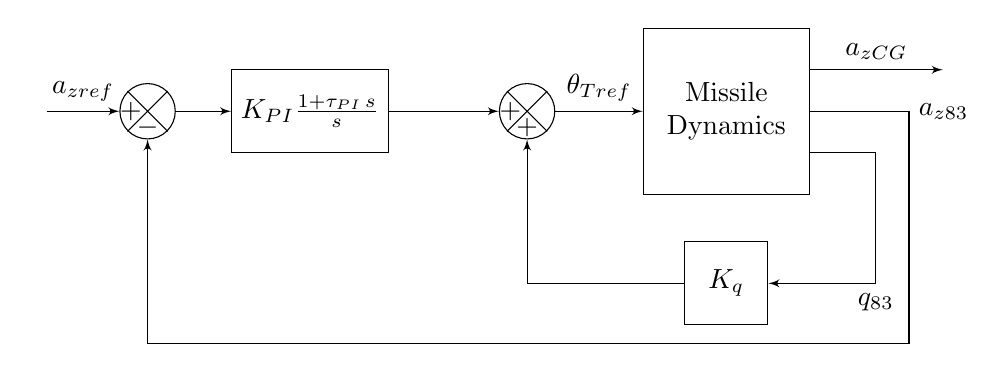
\begin{tikzpicture}

% Entry and first sum
\sbEntree{azref}
\sbComp{errComp}{azref}
	\sbRelier[$a_{zref}$]{azref}{errComp}

% PI block
\sbBlocL{PI}{$K_{PI}\frac{1+\tau_{PI}\,s}{s}$}{errComp}

% Sum PI + Kq
\sbSumb[5]{thetaTref}{PI}
	\sbRelier{PI}{thetaTref}

% Missile
\def \L {6em}
\node[on grid, draw, on grid, align=center, rectangle, minimum height=\L, minimum width=\L] (MIC) [right=\L*1.2 of thetaTref] {Missile\\Dynamics};
\node[on grid, minimum width=\L] (MO1) [above=\L/4 of MIC] {};
\node[on grid, minimum width=\L] (MO3) [below=\L/4 of MIC] {};
	\sbRelier[$\theta_{Tref}$]{thetaTref}{MIC}

% azCG exit
\node (azCG) [right=\L*0.8 of MO1] {};
	\sbRelier[$a_{zCG}$]{MO1}{azCG}

% Gyro measurement
\node[draw, rectangle, minimum height=3em, minimum width=3em] (rateController) [below=of MO3] {$K_{q}$};
\node (rateControllergauche) at (rateController.west){};
\draw[sbStyleLien,auto] (MO3)  --  ++(\L*0.9,0) |- node {$q_{83}$} (rateController);
\sbRelierxy{rateController}{thetaTref}

% Acc measurement and loop
\draw[sbStyleLien,auto] (MIC) -| node {$a_{z83}$} ++(\L*1.1,-\L*1.4) -| (errComp);

\end{tikzpicture}

\caption{Latax Control Architecture\label{fig:RBCL}}


\end{figure}


The pitch rate feedback gain $K_{q}$ is chosen to damp the short
period pitch oscillation (SPPO). On Figure \ref{fig:pitchRateFB}
is shown the root locus of this feedback. It proves that the SPPO
mode changes in damping ratio and very little in natural frequency.
This inner loop must be as fast as possible thus a damping ratio of
0.7 might be appropriate. For a rigid ASTER 30, it yields a pitch
rate feedback gain $K_{q}$ of 0.074.

\begin{figure}
\begin{centering}
\includegraphics[width=0.6\paperwidth]{figures/rlocusKq}
\par\end{centering}

\caption{Root Locus of Pitch Rate Feedback\label{fig:pitchRateFB}}


\end{figure}


The proportional integral corrector on the lateral acceleration $PI(s)=K_{PI}\frac{1+\tau_{PI}s}{s}$
is set to make the system as fast as possible with reasonable gain
and phase margins. For instance, a good compromise is 

\[
PI(s)=0.009\,\frac{1+0.1\,s}{s}
\]
giving a phase margin of $74\text{\textdegree}$ for a rigid ASTER
30. The proportional integral corrector will only make the SPPO natural
frequency lower. Thus, this double loop architecture cannot control
the lateral acceleration faster than the SPPO. The SPPO is the limit
to the lateral acceleration generation.


\section{Vibrations Alleviation\label{sec:vibesAlleviation}}

For agile missiles such as ASTER, the actuators bandwidths are wide.
Thus, if the command signal generated has a non zero component at
the bending frequency, the structural mode will start to oscillate.
This oscillation is measured by the sensors and fed through the controller
which could amplify it. On Figure \ref{fig:rlocusNoVibeSupp} is drawn
the root locus for the system open loop from the nozzle orientation
reference $\theta_{Tref}$ to the pitch rate $q_{83}$ measured at
the sensor pack location, on node 83. The $1^{st}$ and the $3^{rd}$
bending mode can become unstable with this feedback which is supposed
to damp the short period pitch oscillation (SPPO) if the gain is too
important.

\begin{figure}
\begin{centering}
\includegraphics[width=0.6\paperwidth]{figures/rlocusNoVibeSupp2}
\par\end{centering}

\caption{Root Locus of $\frac{q_{83}}{\theta_{Tref}}$\label{fig:rlocusNoVibeSupp}}
\end{figure}


Even if the feedback gains are kept small to avoid a structural instability,
the vibrations created by the rocket engine are amplified through
the structure and measured by the sensors. This amplified signal will
generate parasitic actuations of the thrust vectoring.

There are several strategies to deal with the bending oscillation.
The first one is currently used by missile manufacturers and consists
in filtering the input command to the actuator using a notch filter.
This technique will be developed further in the next subsection. Now
that new sensors have been added on the airframe, the measurements
they provide can be used to actively damp the bending oscillations.
Feedback architectures based on the strain measurement, on pitch rate
measurements and on the accelerometer measurements will be investigated
in the following subsections.


\subsection{Notch Filtering\label{sub:notchFilter}}

A notch filter is applied to the command of the thrust vectoring.
This filter will remove any signal of the bending mode frequency.
The first step is to choose an appropriate type of filter. A Chebyshev
Type II filter suits the problem because there is no ripple in the
bandwidth that could create gain distortion and affect performance
at low frequency. However, this type of filter requires a high order
denominator to ensure a sharp gain loss. The filter centre frequency
is set to 20Hz with a stop-band bandwidth of $\pm10\%$. Indeed, the
uncertainty on the first bending mode frequency is about $\pm10\%$.
The gain loss is set to $40\,dB$. The order of the filter is 4. With
these criteria, the corresponding Chebyshev Type II filter is

\[
N(s)=\frac{s^{4}+\left(3.19\cdot10^{4}\right)\,s^{2}+2.49\cdot10^{8}}{s^{4}+239.0\,s^{3}+\left(6.04\cdot10^{4}\right)\,s^{2}+\left(3.77\cdot10^{6}\right)\,s+2.49\cdot10^{8}}
\]


The Bode diagram of the filter is plotted on Figure \ref{fig:notchFilter}.
The phase loss brought by this notch filter is already $-100{^\circ}$
at $70\,rad.s^{-1}$ that may bring poorer performance even at low
frequencies. A higher order notch filter could also be chosen to obtain
a sharper band-stop.

\begin{figure}
\begin{centering}
\includegraphics[width=0.6\paperwidth]{figures/notchFilter}
\par\end{centering}

\caption{Bode Diagram of the Notch Filter\label{fig:notchFilter}}
\end{figure}


Thanks to this filter, the actuator avoids exciting the first bending
mode and bending oscillations will not generate parasitic actuations.
The bode diagram of $\frac{q_{83}(s)}{\theta_{Tref}(s)}$ is plotted
on Figure \ref{fig:bodeFiltered}. This shows clearly that the resonance
peak of the first bending mode has but cut down by $40\,dB$.

\begin{figure}
\begin{centering}
\includegraphics[width=0.6\paperwidth]{figures/bodeFiltered}
\par\end{centering}

\caption{Bode Diagram of $\frac{q_{83}(s)}{\theta_{Tref}(s)}$\label{fig:bodeFiltered}}


\end{figure}


Once the filter is plugged to the system input, a conventional pitch
rate feedback with a proportional integral controller on the acceleration
can be designed. The new feedback architecture is drawn on Figure
\ref{fig:NFCL}.

\begin{figure}
\begin{centering}
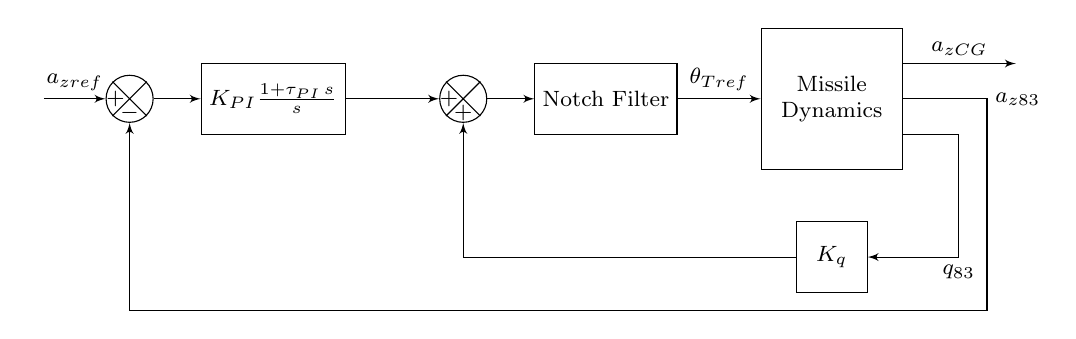
\begin{tikzpicture}
\begin{footnotesize}

% Entry and first sum
\sbEntree{azref}
\sbComp{errComp}{azref}
	\sbRelier[$a_{zref}$]{azref}{errComp}

% PI block
\sbBlocL{PI}{$K_{PI}\frac{1+\tau_{PI}\,s}{s}$}{errComp}

% Sum PI + Kq
\sbSumb[5]{thetaTref}{PI}
	\sbRelier{PI}{thetaTref}

% Notch Filter
\sbBloc{filter}{Notch Filter}{thetaTref}
	\sbRelier{thetaTref}{filter}

% Missile
\def \L {6em}
\node[on grid, draw, on grid, align=center, rectangle, minimum height=\L, minimum width=\L] (MIC) [right=\L*1.6 of filter] {Missile\\Dynamics};
\node[on grid, minimum width=\L] (MO1) [above=\L/4 of MIC] {};
\node[on grid, minimum width=\L] (MO3) [below=\L/4 of MIC] {};
	\sbRelier[$\theta_{Tref}$]{filter}{MIC}

% azCG exit
\node (azCG) [right=\L*0.8 of MO1] {};
	\sbRelier[$a_{zCG}$]{MO1}{azCG}

% Gyro measurement
\node[draw, rectangle, minimum height=3em, minimum width=3em] (rateController) [below=of MO3] {$K_{q}$};
\node (rateControllergauche) at (rateController.west){};
\draw[sbStyleLien,auto] (MO3)  --  ++(\L*0.9,0) |- node {$q_{83}$} (rateController);
\sbRelierxy{rateController}{thetaTref}

% Acc measurement and loop
\draw[sbStyleLien,auto] (MIC) -| node {$a_{z83}$} ++(\L*1.1,-\L*1.5) -| (errComp);

\end{footnotesize}
\end{tikzpicture}
\par\end{centering}

\caption{Closed-Loop with Notch Filter\label{fig:NFCL}}


\end{figure}



\subsection{Active Structural Damping}

The notch filter is a simple solution to deal with vibrations but
it does not remove them. Another way to overcome bending oscillations
is to artificially augment the damping ratio of the bending mode.
This is called active structural damping. 


\subsubsection{Requirements\label{sub:Requirements}}

The controller must generate a force that is opposite to the vibration
speed to damp the bending oscillations. To do so, the controller can
either use the thrust vectoring or the central fins. The natural frequency
of the first mode is 20Hz. The bandwidth of the thrust vectoring is
about 25Hz which is too low: at 20Hz, the thrust vectoring actuator
has a phase loss of -70\textdegree{} and a gain loss of -1.5dB as
shown on Figure \ref{fig:bodeThrustVect}. This is very close to the
cutoff frequency and the real behaviour of the actuator at this frequency
is not accurately modeled.

\begin{figure}
\begin{centering}
\includegraphics[width=0.6\paperwidth]{figures/bodeThrustVect}
\par\end{centering}

\caption{Bode Diagram of $\frac{\theta_{T}(s)}{\theta_{Tref}(s)}$\label{fig:bodeThrustVect}}
\end{figure}


The fins have a bandwidth of 50Hz that is more than the double of
the bending mode frequency. The phase loss at 20Hz is only -34\textdegree{}
and the gain loss is -0.1dB as shown on Figure \ref{fig:bodeFins}.
Therefore this fast actuator is to be preferred for active damping
of the first bending mode. Moreover, the fins are located in the middle
where the flexure is important therefore they have an important controllability
of the first bending mode. Also, at the first bending mode frequency,
the fins deflection have very little influence on the slow rigid-body
dynamics. Moreover, they are located close to the centre of gravity
so they do not create a big change in the angle of attack. The fins
will be used to actively damp the bending vibrations.

\begin{figure}
\begin{centering}
\includegraphics[width=0.6\paperwidth]{figures/bodeFins}
\par\end{centering}

\caption{Bode Diagram of $\frac{\delta_{F}(s)}{\delta_{Fref}(s)}$\label{fig:bodeFins}}


\end{figure}



\subsubsection{Strain Feedback}

The strain gauge is a sensor that is usually not present on a missile
airframe. With this extra sensor, it possible to measure the local
strain on the skin of the structure to infer on its flexure. This
additional information can help to deal with bending oscillation.
If only the first bending mode is considered, the transfer function
of the fins deflection to the strain can be approximated to:

\[
\frac{\varepsilon_{46}}{\delta_{F}}(s)=K_{\nicefrac{\varepsilon}{\delta_{F}}}\frac{\omega_{1}^{2}}{s^{2}+2\,\zeta_{1}\,\omega_{1}\,s+\omega_{1}^{2}}
\]


To increase the term $\zeta_{1}$ with a simple feedback, the strain
measurement needs to be derivated as shown in the block diagram in
Figure \ref{fig:strainFB1}. The transfer function of the closed-loop
would then be 

\[
\left(\frac{\varepsilon_{46}}{\delta_{F}}\right)_{CL}(s)=K_{\nicefrac{\varepsilon}{\delta_{F}}}\frac{\omega_{1}^{2}}{s^{2}+2\,(\zeta_{1}+\frac{1}{2}K_{\nicefrac{\varepsilon}{\delta_{F}}}\omega_{1}K_{\varepsilon})\,\omega_{1}\,s+\omega_{1}^{2}}
\]


\begin{figure}
\begin{centering}
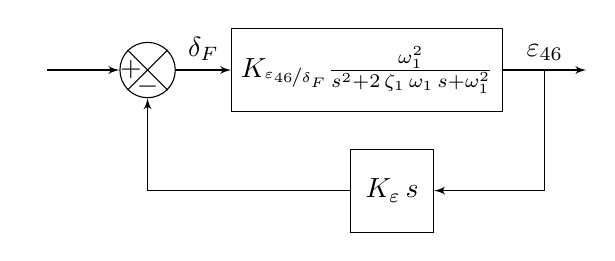
\begin{tikzpicture}

% Entry and first sum
\sbEntree{entree}
\sbComp{errComp}{entree}
	\sbRelier{entree}{errComp}

% Actuator and exit
\sbBloc{tf}
{$K_{\nicefrac{\varepsilon_{46}}{\delta_{F}}}\frac{\omega_{1}^{2}}{s^{2}+2\,\zeta_{1}\,\omega_{1}\,s+\omega_{1}^{2}}$}
{errComp}
	\sbRelier[$\delta_{F}$]{errComp}{tf}
\sbSortie[3]{epsilon}{tf}
	\sbRelier[$\varepsilon_{46}$]{tf}{epsilon}

% Strain feedback
\sbDecaleNoeudy{tf-epsilon}{corner}
\sbBlocr[4]{corr}{$K_{\varepsilon}\,s$}{corner}
	\sbRelieryx{tf-epsilon}{corr}
	\sbRelierxy{corr}{errComp}

\end{tikzpicture}
\par\end{centering}

\caption{Block Diagram of Derivative Strain Feedback\label{fig:strainFB1}}
\end{figure}


The feedback gain $K_{\varepsilon}$ directly changes the damping
ratio of the first bending mode without changing the static gain $K_{\nicefrac{\varepsilon}{\delta_{F}}}$
or the natural frequency $\omega_{1}$. However this feedback is non
causal and a pole needs to be added. This artificial pole can be placed
very fast to minimize its influence on the dynamics. The feedback
transfer function would then be
\[
K_{\varepsilon}\,\frac{s}{1+\nicefrac{s}{\omega_{fast}}}
\]


This feedback loop would work if the fins actuator was very fast.
This is not the case because even if its bandwidth is twice bigger
than the bending mode natural frequency, the phase loss is non negligible
as shown in \ref{sub:Requirements}.

Fortunately with this phase shift a simple proportional feedback will
damp the bending oscillations. On Figure \ref{fig:rlocusStrain},
a root locus has been plotted with the full dynamics of all 5 bending
modes, flight dynamics and actuator dynamics. With a proportional
feedback gain of 600, the damping ratio of the first bending mode
has been increased by 10 to 12.5\%. This gain is chosen to obtain
a gain margin of 6dB and a phase margin of 30\textdegree .

\begin{figure}
\begin{centering}
\includegraphics[width=0.6\paperwidth]{figures/rlocusStrain}
\par\end{centering}

\caption{Root Locus of $\frac{\varepsilon_{46}}{\delta_{Fref}}(s)$\label{fig:rlocusStrain}}


\end{figure}


With this first loop, the bode diagram of $\frac{q_{83}}{\theta_{Tref}}(s)$
on Figure \ref{fig:bodeDampingStrain} shows that the first bending
mode is clearly damped. The resonance peak at $125\,rad.s^{-1}$ has
been cut down thoroughly by $20\,dB$.

\begin{figure}
\begin{centering}
\includegraphics[width=0.6\paperwidth]{figures/bodeDampingStrain}
\par\end{centering}

\caption{Bode of $\frac{q_{83}}{\theta_{Tref}}(s)$ With and Without Strain
Feedback\label{fig:bodeDampingStrain}}


\end{figure}


This active damping replaces the notch filter seen in \vref{sub:notchFilter}.
The complete feedback architecture containing the strain feedback,
the pitch rate loop and the proportional integrator corrector is on
Figure \ref{fig:completeStrainFB}.

\begin{figure}
\begin{centering}
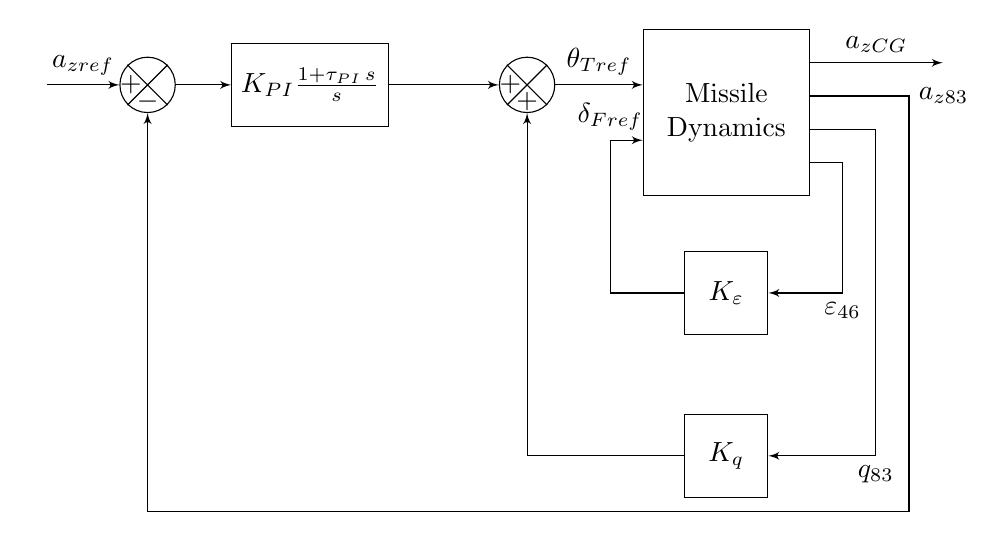
\begin{tikzpicture}

% Entry and first sum
\sbEntree{azref}
\sbComp{errComp}{azref}
	\sbRelier[$a_{zref}$]{azref}{errComp}

% PI block
\sbBlocL{PI}{$K_{PI}\frac{1+\tau_{PI}\,s}{s}$}{errComp}

% Sum PI + Kq
\sbSumb[5]{thetaTref}{PI}
	\sbRelier{PI}{thetaTref}

% Missile
\def \L {6em}
\node[on grid, minimum width=\L] (MI1) [right=\L*1.2 of thetaTref] {};
\node[draw, on grid, align=center, rectangle, minimum height=\L, minimum width=\L] (MIC) [below=\L/6 of MI1] {Missile\\Dynamics};
\node[on grid, minimum width=\L] (MI2) [below=\L/6 of MIC] {};
\node[on grid, minimum width=\L] (MO1) [above=\L*3/10 of MIC] {};
\node[on grid, minimum width=\L] (MO2) [above=\L*1/10 of MIC] {};
\node[on grid, minimum width=\L] (MO3) [below=\L*1/10 of MIC] {};
\node[on grid, minimum width=\L] (MO4) [below=\L*3/10 of MIC] {};
	\sbRelier[$\theta_{Tref}$]{thetaTref}{MI1}

% azCG exit
\node (azCG) [right=\L*0.8 of MO1] {};
	\sbRelier[$a_{zCG}$]{MO1}{azCG}

% Strain measurement
\node[draw, rectangle, minimum height=3em, minimum width=3em] (strainController) [below=of MO4] {$K_{\varepsilon}$};
\node (strainControllergauche) at (strainController.west){};
\draw[sbStyleLien,auto] (MO4)  --  ++(\L*0.7,0) |- node {$\varepsilon_{46}$} (strainController);
\draw[sbStyleLien,auto] (strainController)  --  ++(-\L*0.7,0) |- node {$\delta_{Fref}$} (MI2);


% Gyro measurement
\node[draw, rectangle, minimum height=3em, minimum width=3em] (rateController) [below=of strainController] {$K_{q}$};
\node (rateControllergauche) at (rateController.west){};
\draw[sbStyleLien,auto] (MO3)  --  ++(\L*0.9,0) |- node {$q_{83}$} (rateController);
\sbRelierxy{rateController}{thetaTref}

% Acc measurement and loop
\draw[sbStyleLien,auto] (MO2) -| node {$a_{z83}$} ++(\L*1.1,-\L*2.5) -| (errComp);

%\sbBloc{sys}{System}{entree}
%\sbDecaleNoeudy[0.5]{sys}{a}
%\sbDecaleNoeudy[-0.5]{sys}{b}

%\sbBloc[5]{out1}{out1}{a}
%	\sbRelier[out1]{a}{out1}
%\sbBloc[5]{out2}{out2}{b}
%	\sbRelier[out2]{b}{out2}
%\sbStyleBloc{fill=white}
%\sbBloc{sysbis}{System}{entree}
%\sbStyleBlocDefaut

\end{tikzpicture}
\par\end{centering}

\caption{Feedback Architecture with Strain Gauges\label{fig:completeStrainFB}}


\end{figure}


This feedback architecture has some disadvantages though. The strain
measured is not only coming from bending deformations. Some longitudinal
or twisting modes may create local strains and propagate noise in
the system. Moreover, without an appropriate band-pass filter, the
static bending will create a static deflection of the fins and increase
drag.


\subsubsection{Gyroscope Feedback}

Two gyroscopes can give information on the flexure. A gyroscope is
placed at the rear and the other one is the gyroscope included in
the sensor pack next to the nose. The problem with damping bending
with gyroscopes is that they measure not only the local pitch rate
of the bending but also the rigid-body pitch rate. Thus two of them
are needed to subtract the rigid-body pitch rate. Indeed, a gyro at
node $i$ will measure $q_{i}=q_{RB}+q_{FBi}$. The subtraction of
the signals coming from the two gyroscopes will give:

\[
q_{10}-q_{83}=q_{fb,10}-q_{fb,83}=\Delta q
\]


If only the first bending mode is considered, the transfer function
of the fins deflection $\delta_{F}$ to the pitch rate difference
$\Delta q$ is

\[
\frac{\Delta q}{\delta_{F}}(s)=K_{\nicefrac{\Delta q}{\delta_{F}}}\frac{\omega_{1}^{2}\,s}{s^{2}+2\,\zeta_{1}\,\omega_{1}\,s+\omega_{1}^{2}}
\]
thus with a simple proportional feedback gain $K_{\Delta q}$ from
$\Delta q$ to $\delta_{F}$ would modify the transfer function to
\[
\left(\frac{\Delta q}{\delta_{F}}\right)_{CL}(s)=K_{\nicefrac{\Delta q}{\delta_{F}}}\frac{\omega_{1}^{2}\,s}{s^{2}+2\,(\zeta_{1}+\frac{1}{2}\,K_{\nicefrac{\Delta q}{\delta_{F}}}\omega_{1}K_{\Delta q})\,\omega_{1}\,s+\omega_{1}^{2}}
\]


This feedback would damp the first bending mode without modifying
the other parameters. Now considering the phase loss of the actuator
of about 30\textdegree , the natural frequency of the first bending
mode will change but damping is still possible. On Figure \ref{fig:rlocusDGyr}
the root locus of $\frac{\Delta q}{\delta_{Fref}}(s)$ shows that
a damping of 12\% on the first bending mode can be achieved with a
feedback gain $K_{\Delta q}=0.24$.

\begin{figure}
\begin{centering}
\includegraphics[width=0.6\paperwidth]{figures/rlocusDGyr}
\par\end{centering}

\caption{Root Locus of $\frac{\Delta q}{\delta_{Fref}}(s)$\label{fig:rlocusDGyr}}
\end{figure}


The effect of this loop on the resonance peak of the first bending
mode can be seen on Figure \ref{fig:bodeDampingGyr}. The resonance
peak is reduced by $20\,dB$.

\begin{figure}
\begin{centering}
\includegraphics[width=0.6\paperwidth]{figures/bodeDampingGyr}
\par\end{centering}

\caption{Bode of $\frac{q_{83}}{\theta_{Tref}}(s)$ With and Without $\Delta q$
Feedback\label{fig:bodeDampingGyr}}
\end{figure}


To this damping loop are added the conventional feedbacks on the pitch
rate and the lateral acceleration. The complete architecture in this
case is draw on Figure \ref{fig:completeGyrFB}.

\begin{figure}
\begin{centering}
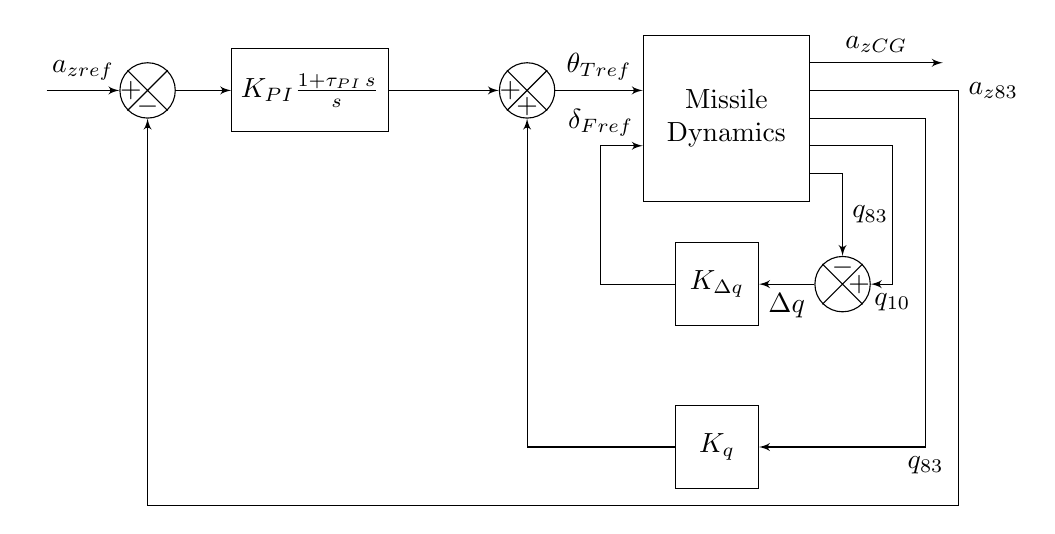
\begin{tikzpicture}

% Entry and first sum
\sbEntree{azref}
\sbComp{errComp}{azref}
	\sbRelier[$a_{zref}$]{azref}{errComp}

% PI block
\sbBlocL{PI}{$K_{PI}\frac{1+\tau_{PI}\,s}{s}$}{errComp}

% Sum PI + Kq
\sbSumb[5]{thetaTref}{PI}
	\sbRelier{PI}{thetaTref}

% Missile
\def \L {6em}
\node[on grid, minimum width=\L] (MI1) [right=\L*1.2 of thetaTref] {};
\node[draw, on grid, align=center, rectangle, minimum height=\L, minimum width=\L] (MIC) [below=\L/6 of MI1] {Missile\\Dynamics};
\node[on grid, minimum width=\L] (MI2) [below=\L/6 of MIC] {};
\node[on grid, minimum width=\L] (MO1) [above=\L*1/3 of MIC] {};
\node[on grid, minimum width=\L] (MO2) [above=\L*1/6 of MIC] {};
\node[on grid, minimum width=\L] (MO4) [below=\L*1/6 of MIC] {};
\node[on grid, minimum width=\L] (MO5) [below=\L*1/3 of MIC] {};
	\sbRelier[$\theta_{Tref}$]{thetaTref}{MI1}

% MO4 & MO5 preparation
\node (MO4droite) at (MO4.east){};
\node (MO5droite) at (MO5.east){};

% azCG exit
\node (azCG) [right=\L*0.8 of MO1] {};
	\sbRelier[$a_{zCG}$]{MO1}{azCG}

% Delta gyr
\node [on grid, draw, circle,minimum size=2em, below right=\L and \L*0.7 of MIC] (sumGyr) {};
\node [on grid, draw, cross out,minimum size=1.414em] at (sumGyr) {};
\node [above of=sumGyr,node distance=0.6em] {$-$};
\node [below of=sumGyr,node distance=0.6em] {};
\node [left of=sumGyr,node distance=0.6em] {};
\node [right of=sumGyr,node distance=0.6em] {$+$};
\node (symGyrdroite) at (sumGyr.east){};
\node (sumGyrgauche) at (sumGyr.west){};
	\sbRelierxy[$q_{83}$]{MO5}{sumGyr};
	\draw[sbStyleLien,auto] (MO4)  --  ++(\L,0) |- node {$q_{10}$} (sumGyr);

% Delta gyr controller
\sbBlocr{dGyrController}{$K_{\Delta q}$}{sumGyr};
\sbRelier[$\Delta q$]{sumGyr}{dGyrController};
\draw[sbStyleLien,auto] (dGyrController)  --  ++(-\L*0.7,0) |- node {$\delta_{Fref}$} (MI2);


% Gyro measurement
\node[draw, rectangle, minimum height=3em, minimum width=3em] (rateController) [below=of dGyrController] {$K_{q}$};
\node (rateControllergauche) at (rateController.west){};
\draw[sbStyleLien,auto] (MIC)  --  ++(\L*1.2,0) |- node {$q_{83}$} (rateController);
\sbRelierxy{rateController}{thetaTref}

% Acc measurement and loop
\draw[sbStyleLien,auto] (MO2) -| node {$a_{z83}$} ++(\L*1.4,-\L*2.5) -| (errComp);

\end{tikzpicture}
\par\end{centering}

\caption{Feedback Architecture with Gyroscopes\label{fig:completeGyrFB}}
\end{figure}


This controller architecture has the disadvantage that the two gyroscopes
must be similarly calibrated and synchronized to perform the subtraction
correctly. The great advantage is the absence of fins deflection in
static.


\subsubsection{Accelerometer Feedback\label{sub:Accelerometer-Feedback}}

Using accelerometers for the feedback is more complicated than using
gyroscopes. At node $i$, the accelerometer will measure $a_{z,i}=a_{z,CG}+(x_{CG}-x_{i})\,\dot{q}+a_{zi,fb}$.
There are three unknowns in this equality: $a_{z,CG}$, $\dot{q}$,
and $a_{zi,fb}$ hence three uncorrelated accelerometers are needed
to keep only the flexible body component. On the airframe, three accelerometers
have been added at node 10, 53 and 92. Considering only the first
bending mode, all the $a_{zi,fb}$ are proportional to the first bending
mode mean acceleration $a_{z,m1}$. A linear combination of these
three measurements must be found so that it does not depend of $a_{z,CG}$
and $\dot{q}$. Let ($c_{10}$, $c_{53}$, $c_{92}$) be three coefficients
so that
\[
c_{10}a_{z,10}+c_{53}a_{z,53}+c_{92}a_{z,92}=c\,a_{z,m1}
\]
where $c$ is a non zero real number. Let say that $c_{10}=1$ to
make the linear system of Cramer. In a matrix form, this gives 
\[
\left[\begin{array}{ccc}
1 & 1 & 1\\
9 & 52 & 91\\
1 & 0 & 0
\end{array}\right]\left[\begin{array}{c}
c_{10}\\
c_{53}\\
c_{92}
\end{array}\right]=\left[\begin{array}{c}
0\\
0\\
1
\end{array}\right]
\]


The solution is $\left[\begin{array}{c}
c_{10}\\
c_{53}\\
c_{92}
\end{array}\right]=\left[\begin{array}{c}
1\\
-\nicefrac{82}{39}\\
\nicefrac{43}{39}
\end{array}\right].$ The linear combination $c_{10}a_{z,10}+c_{53}a_{z,53}+c_{92}a_{z,92}$
will be called $\sum a_{z}$. The transfer function of the fins deflection
to this linear combination of accelerations is of the form
\[
\frac{\sum a_{z}}{\delta_{F}}(s)=K_{\nicefrac{\sum a_{z}}{\delta_{F}}}\frac{\omega_{1}^{2}\,s^{2}}{s^{2}+2\,\zeta_{1}\,\omega_{1}\,s+\omega_{1}^{2}}
\]
hence to damp the first bending mode, the feedback needs an integrator
so that the resulting transfer function would be

\[
\frac{\sum a_{z}}{\delta_{F}}_{CL}(s)=K_{\nicefrac{\sum a_{z}}{\delta_{F}}}\frac{\omega_{1}^{2}\,s^{2}}{s^{2}+2\,(\zeta_{1}+K_{\nicefrac{\sum a_{z}}{\delta_{F}}}\omega_{1}K_{a_{z}})\,\omega_{1}\,s+\omega_{1}^{2}}
\]


Like for the gyroscopes, the phase loss of the fins actuator will
generate a change in the bending oscillation natural frequency. The
root locus of $\frac{1}{s}\,\frac{\sum a_{z}}{\delta_{F}}$ is plotted
on Figure \ref{fig:rlocusSAcc} and shows that the first bending mode
can be damped to 12\% with a gain $K_{a_{z}}$ of 0.16.

\begin{figure}
\begin{centering}
\includegraphics[width=0.6\paperwidth]{figures/rlocusSAcc}
\par\end{centering}

\caption{Root Locus of $\frac{1}{s}\frac{\sum a_{z}}{\delta_{Fref}}(s)$\label{fig:rlocusSAcc}}
\end{figure}


A comparative Bode plot shows on Figure \ref{fig:bodeDampingAcc}
the effect of such a damping architecture. Once again the resonance
peak has been cut off.

\begin{figure}
\begin{centering}
\includegraphics[width=0.6\paperwidth]{figures/bodeDampingAcc}
\par\end{centering}

\caption{Bode of $\frac{q_{83}}{\theta_{Tref}}(s)$ With and Without $\sum a_{z}$
Feedback\label{fig:bodeDampingAcc}}
\end{figure}


The complete controller architecture is drawn in Figure \ref{fig:completeAccFB}.

\begin{figure}
\begin{centering}
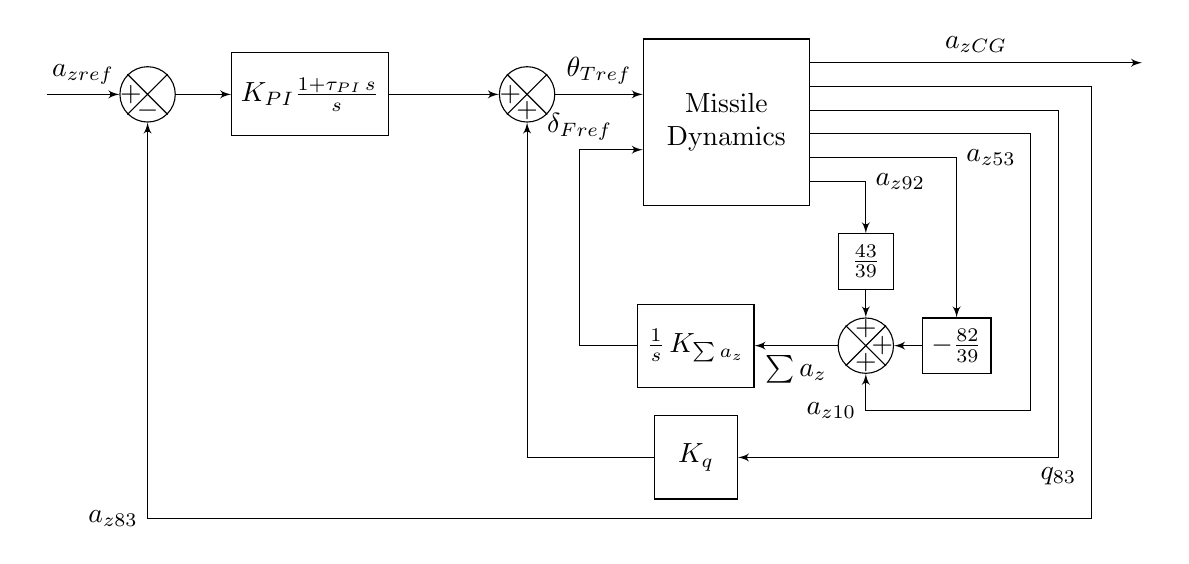
\begin{tikzpicture}

% Entry and first sum
\sbEntree{azref}
\sbComp{errComp}{azref}
	\sbRelier[$a_{zref}$]{azref}{errComp}

% PI block
\sbBlocL{PI}{$K_{PI}\frac{1+\tau_{PI}\,s}{s}$}{errComp}

% Sum PI + Kq
\sbSumb[5]{thetaTref}{PI}
	\sbRelier{PI}{thetaTref}

% Missile
\def \L {6em}
\node[on grid, minimum width=\L] (MI1) [right=\L*1.2 of thetaTref] {};
\node[draw, on grid, align=center, rectangle, minimum height=\L, minimum width=\L] (MIC) [below=\L/6 of MI1] {Missile\\Dynamics};
\node[on grid, minimum width=\L] (MI2) [below=\L/6 of MIC] {};
\node[on grid, minimum width=\L] (MO1) [above=\L*5/14 of MIC] {};
\node[on grid, minimum width=\L] (MO2) [above=\L*3/14 of MIC] {};
\node[on grid, minimum width=\L] (MO3) [above=\L*1/14 of MIC] {};
\node[on grid, minimum width=\L] (MO4) [below=\L*1/14 of MIC] {};
\node[on grid, minimum width=\L] (MO5) [below=\L*3/14 of MIC] {};
\node[on grid, minimum width=\L] (MO6) [below=\L*5/14 of MIC] {};
	\sbRelier[$\theta_{Tref}$]{thetaTref}{MI1}

% azCG exit
\node (azCG) [right=\L*2 of MO1] {};
	\sbRelier[$a_{zCG}$]{MO1}{azCG}

% Gains
% Gain 92
\node[draw, align=center, rectangle, minimum height=2em, minimum width=2em] (k92) [below right=\L/6 and \L/6 of MIC] {$\frac{43}{39}$};
\draw[sbStyleLien,auto] (MO6) -| node {$a_{z92}$} (k92);

% Gain 53
\node[draw, align=center, rectangle, minimum height=2em, minimum width=2em] (k53) [below right=1em and 1em of k92] {$-\frac{82}{39}$};
\draw[sbStyleLien,auto] (MO5) -| node {$a_{z53}$} (k53);

% Sum Acc
\node [draw, circle,minimum size=2em, below =1em of k92] (sumAcc) {};
\node [on grid, draw, cross out,minimum size=1.414em] at (sumAcc) {};
\node [above of=sumAcc,node distance=0.6em] {$+$};
\node [below of=sumAcc,node distance=0.6em] {$+$};
\node [left of=sumAcc,node distance=0.6em] {};
\node [right of=sumAcc,node distance=0.6em] {$+$};
\node (symAccdroite) at (sumAcc.east){};
\node (sumAccgauche) at (sumAcc.west){};
	\draw[sbStyleLien,auto] (k92) -- (sumAcc);
	\draw[sbStyleLien,auto] (k53) -- (sumAcc);
	\draw[sbStyleLien,auto] (MO4)  -|  ++(11em,-10em) -| node {$a_{z10}$} (sumAcc);

% Sum acc controller
\sbBlocr[3]{sAccController}{$\frac{1}{s}\,K_{\sum a_z}$}{sumAcc};
\sbRelier[$\sum a_z$]{sumAcc}{sAccController};
\draw[sbStyleLien,auto] (sAccController)  --  ++(-\L*0.7,0) |- node {$\delta_{Fref}$} (MI2);

% Gyro measurement
\node[draw, rectangle, minimum height=3em, minimum width=3em] (rateController) [below=1em of sAccController] {$K_{q}$};
\node (rateControllergauche) at (rateController.west){};
\draw[sbStyleLien,auto] (MO3)  --  ++(2*\L,0) |- node {$q_{83}$} (rateController);
\sbRelierxy{rateController}{thetaTref}

% Acc measurement and loop
\draw[sbStyleLien,auto] (MO2) -| ++(\L*2.2,-\L*2.6) -| node {$a_{z83}$} (errComp);

\end{tikzpicture}
\par\end{centering}

\caption{Feedback Architecture with Accelerometers\label{fig:completeAccFB}}
\end{figure}


Using accelerometers for structural damping might bring some problems
because the accelerometers must be similarly calibrated and synchronized
like the gyroscopes. The position of the centre of gravity does not
need to be known. Indeed when the linear equation system has been
solved, the solution do not depend on the centre of gravity location.
The integration will reduce parasitic actuation of the fins due to
noise at high frequency.


\section{H$_{\infty}$ Fixed-Structure Tuning}

Four controller architectures will be assessed. They all have in common
the lateral acceleration control composed of a pitch rate feedback
and a proportional integral controller on the lateral acceleration.
The first architecture has a notch filter. The controller number 2
to 4 use active damping with respectively:
\begin{itemize}
\item the strain gauge feedback,
\item the 2-gyroscope feedback,
\item the 3-accelerometer feedback.
\end{itemize}
These controllers will be respectively denoted ``Notch'', ``Strain'',
``Gyro'' and ``Acc''.

These architectures will be tuned using the same criteria to eventually
compare their performance. The method will use the $H_{\infty}$-tuning
for fixed-structure controllers developed by P. Apkarian in \cite{apkarian2006nonsmooth}.

Each architecture is put in a weighted form like on Figure \ref{fig:HinfForm}.
The input to the closed-loop system is the exogenous vector $w$ which
contains all the inputs like noises, perturbations or references.
The output is the performance vector $z$ containing all the performance
indices that one will minimize. The diagonal matrices $W_{in}$ and
$W_{out}$ are weights applied to $w$ and $z$ to define the requirements.
The algorithm will tune the controller gains in order to make the
system stable while minimizing $\gamma$ such that 
\[
\left\Vert W_{out}HW_{in}\right\Vert _{\infty}<\gamma
\]


\begin{figure}
\begin{centering}
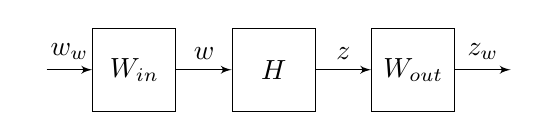
\begin{tikzpicture}

% Entry and first sum
\sbEntree{ww}

\sbBloc{Ww}{$W_{in}$}{ww}
	\sbRelier[$w_{w}$]{ww}{Ww}

\sbBloc{G}{$H$}{Ww}
	\sbRelier[$w$]{Ww}{G}

\sbBloc{Wz}{$W_{out}$}{G}
	\sbRelier[$z$]{G}{Wz}

% zw exit
\sbSortie{zw}{Wz};
	\sbRelier[$z_{w}$]{Wz}{zw}

\end{tikzpicture}
\par\end{centering}

\caption{Weighted Form for $H_{\infty}$-tuning\label{fig:HinfForm}}
\end{figure}


The parameters subject to tuning are $K_{q}$, $K_{PI}$ and $\tau_{PI}$.
The notch filter, the strain feedback, the gyroscope feedback or the
accelerometer feedback are not tunable. They are defined in \vref{sec:vibesAlleviation}.

The exogenous vector $w$ only contains the reference lateral acceleration
$a_{zref}$. The corresponding weight is set to 1. Thus, the other
signals weights will be chosen according to a reference acceleration
of $1\,m.s^{-1}$. Additional inputs are not needed, first of all
because the tuning needs to be simple but also because other inputs
like noise, actuators perturbations or gust perturbations are neglected.
The sensors noise is very low compared to signals generated by vibrations.
The fins actuator perturbations is assumed to be very few compared
to the thrust vectoring perturbations which will not be considered
for tuning but later for assessment. Finally, gusts have a speed which
is negligible compared to the missile speed of Mach 2.

The performance vector $z$ is composed of two signals: the lateral
acceleration error $a_{zref}-a_{zCG}$ and the thrust vectoring orientation
$\theta_{T}$. It is obvious that the lateral acceleration error is
needed in $z$ to design a lateral acceleration controller. The thrust
vectoring orientation $\theta_{T}$ is added in $z$ to limit the
use of this actuator which has a rate limit, a deflection limit and
second-order dynamics. The output weight matrix $W_{out}$ is then
\[
\left[\begin{array}{cc}
W_{err} & 0\\
0 & W_{\theta_{T}}
\end{array}\right]
\]


$W_{err}$ is set to minimize the error at low frequency and bound
it at high frequency for resonance reduction. The controller is equipped
with an integrator so the error will tend to 0. An empirical tuning
of this weight is 

\[
W_{err}(s)=\frac{5}{s}\,\left(\frac{s}{10}+1\right)
\]
which will force the bandwidth to be 5 rad/s. And the maximum error
will be 2 times the reference acceleration. The target shape of $H_{a_{zref}\rightarrow\left(a_{zref}-a_{zCG}\right)}(s)$
will be the inverse of $W_{err}(s)$ and is plotted in Figure \ref{fig:weights}.

\begin{figure}
\begin{centering}
\includegraphics[width=0.5\paperwidth]{figures/weights}
\par\end{centering}

\caption{Singular Values of $\nicefrac{1}{W_{err}(s)}$\label{fig:weights}}
\end{figure}


$W_{\theta_{T}}$ is chosen avoid using the actuator over its cutoff
frequency. A simple way to do this is to chose 
\[
W_{\theta_{T}}(s)=2\cdot10^{-3}\left(\frac{s}{\omega_{T}}\right)^{2}\left(\frac{1}{1+10^{-5}s}\right)^{2}
\]
 where $\omega_{T}$ is the thrust vectoring cutoff frequency of 25Hz
(157 rad/s). The coefficient $2\cdot10^{-3}$ is empirically set.
To have a causal weight, two fast poles are added. Once again, the
target shape of $H_{a_{zref}\rightarrow\theta_{T}}(s)$ is $\nicefrac{1}{W_{\theta_{T}}(s)}$.
The rotation speed of the thrust vectoring must also be bounded. The
system being linear, trying to minimize $\theta_{T}$ will also minimise
$\dot{\theta_{T}}$. The corresponding bound will be $\nicefrac{s}{W_{\theta_{T}}}$

The H$_{\infty}$-tuning yields parameters summarized in Table \ref{tab:HinfstructParam}.
The algorithm found a minimum $\gamma$ between 1.06 (Notch) and 1.2
(Strain). This $\gamma$ is 1.09 for Gyro and Acc architectures

\begin{table}
\begin{centering}
\begin{tabular}{|c|c|c|c|}
\hline 
Controller & $K_{q}\,\left(s\right)$ & $K_{PI}\,\left(\nicefrac{rad\cdot s}{m}\right)$ & $\tau_{PI}\,(s)$\tabularnewline
\hline 
\hline 
Notch & $9.47\cdot10^{-2}$ & $9.46\cdot10^{-3}$ & $0.171$\tabularnewline
\hline 
Strain & $9.98\cdot10^{-2}$ & $13.0\cdot10^{-3}$ & $0.122$\tabularnewline
\hline 
Gyro & $8.40\cdot10^{-2}$ & $9.11\cdot10^{-3}$ & $0.149$\tabularnewline
\hline 
Acc & $8.38\cdot10^{-2}$ & $9.05\cdot10^{-3}$ & $0.151$\tabularnewline
\hline 
\end{tabular}
\par\end{centering}

\caption{H$_{\infty}$-tuned Controllers Parameters \label{tab:HinfstructParam}}
\end{table}


These settings in Table \ref{tab:HinfstructParam} are very similar
especially for the controllers alleviating vibrations. These controllers
will be assessed and compared in the Section \ref{sec:Assessment}.


\section{Controllers Assessment and Comparison\label{sec:Assessment}}


\subsection{Robustness to Uncertainty}

The first criteria to assess is robustness to uncertainty. The H$_{\infty}$
algorithm found stable solutions for the five architectures but they
can turn unstable with some parameters variation. 

The uncertainty has been defined considering the thrust, the centre
of gravity, the bending modes natural frequencies and their damping
ratios as uncertain parameters. The thrust is generated by the rocket
engine and is then very uncertain. The centre of gravity moves along
the flight because of the propellant combustion. Finally the bending
modes natural frequency and especially damping are often poorly identified
and they vary. These parameters uncertainties are summarized in Table
\ref{tab:Parameters-Uncertainty}. Other parameters could also be
defined as uncertain like the actuators bandwidth, the modes shapes,
the aerodynamic coefficients and so on but this should require a specific
study.

\begin{table}
\begin{centering}
\begin{tabular}{|c|c|}
\hline 
Parameter & Uncertainty\tabularnewline
\hline 
\hline 
Thrust magnitude $T_{0}$ & $\pm10\%$\tabularnewline
\hline 
Center of gravity location $x_{CG}$ & $0\text{ to }+10\%$\tabularnewline
\hline 
$i^{th}$ bending mode frequency $\omega_{i}$ & $\pm10\%$\tabularnewline
\hline 
$i^{th}$ bending mode damping ratio $\zeta_{i}$ & $\pm20\%$\tabularnewline
\hline 
\end{tabular}
\par\end{centering}

\caption{Parameters Uncertainty\label{tab:Parameters-Uncertainty}}


\end{table}


To assess robustness, gain margin and phase margin are of little help
for such a MIMO system. Each uncertain system is an infinite set of
possible realisation. A finite subset of systems is created from this
uncertain system and their poles are plotted on Figure \ref{fig:uncertaintyPoles}.
The poles keep a reasonable margin with the imaginary axis. These
closed-loop systems are robust to the designed uncertainty.

\begin{figure}
\begin{centering}
\begin{tabular}{cc}
\includegraphics[width=0.45\textwidth]{figures/pznotch} & \includegraphics[width=0.45\textwidth]{figures/pzstrain}\tabularnewline
Architecture Notch & Architecture Strain\tabularnewline
 & \tabularnewline
\end{tabular}
\par\end{centering}

\begin{centering}
\begin{tabular}{cc}
\includegraphics[width=0.45\textwidth]{figures/pzgyr} & \includegraphics[width=0.45\textwidth]{figures/pzacc}\tabularnewline
Architecture Gyro & Architecture Acc\tabularnewline
\end{tabular}
\par\end{centering}

\caption{Poles of Closed Loop 1 to 4 Subject to Uncertainty\label{fig:uncertaintyPoles}}


\end{figure}



\subsection{Tracking}

The tracking performance of these 4 closed-loop is their ability to
generate a lateral acceleration equal to the reference acceleration.
Step responses give a good insight to assess the tracking performance.
These responses are plotted on Figure \ref{fig:stepErr}.

\begin{figure}
\begin{centering}
\includegraphics[height=0.4\textheight]{figures/step}
\par\end{centering}

\caption{Step Response of $a_{zref}$ to $(a_{zref}-a_{zCG})$\label{fig:stepErr}}


\end{figure}


Another index for tracking performance is the singular values of the
transfer function from the reference acceleration $a_{zref}$ and
the error $a_{zref}-a_{zCG}$ which is on Figure \ref{fig:sigmaErr}.

\begin{figure}
\begin{centering}
\includegraphics[height=0.4\textheight]{figures/sigmaErr}
\par\end{centering}

\caption{Sigma Plot of $a_{zref}$ to $(a_{zref}-a_{zCG})$\label{fig:sigmaErr}}


\end{figure}


Looking at these too figures, the four different closed-loop architectures
yield very similar tracking performance. The rise time from 10 to
90\% following a step demand is between $0.214$ and $0.227\,s$ and
the 2\% settling time is between $0.400$ and $0.406\,s$. The sigma
plots provide information about tracking performance over all frequencies.
The presence of an integrator in the loop gives makes the error converge
to zero at low frequencies. The bandwidth at -3dB is between 3.2 and
3.7 $rad.s^{-1}$.


\subsection{Actuators Demand}

The thrust nozzles cylinders and the fins actuators have second order
dynamics and actuators demand must be limited at high frequency. These
demands must also be limited over the whole range of frequencies to
save energy and to avoid actuators heating and damage.


\subsubsection{Demand for Lateral Acceleration}

The actuators demand following a lateral acceleration command must
be appropriately bounded. The weight $W_{\theta_{T}}$ ensures that
the position and rate of the thrust vectoring stays bounded under
a reasonable threshold. The thrust vectoring demand is plotted on
Figure \ref{fig:sigmaThrust} with respect to frequency.

\begin{figure}
\begin{centering}
\includegraphics[height=0.4\textheight]{figures/sigThetaDemand}
\par\end{centering}

\caption{Singular Values of $a_{zref}$ to $\theta_{T}$\label{fig:sigmaThrust}}
\end{figure}


None of these four architectures cross the threshold imposed by $\nicefrac{1}{W_{\theta_{T}}}$.
The ``Notch'' architecture has a thorough stop-band around the 1st
bending mode natural frequency of 125 rad/s. The three active damping
architectures keep a satisfactory margin. Similarly for the fins actuator,
Figure \ref{fig:sigmaFins} shows the fins deflection for the closed-loops
performing active damping. 

\begin{figure}
\begin{centering}
\includegraphics[height=0.4\textheight]{figures/sigDeltaDemand}
\par\end{centering}

\caption{Singular Values of $a_{zref}$ to $\delta_{F}$\label{fig:sigmaFins}}
\end{figure}


The ``Strain'' architecture generate greater commands on the fins
deflection at frequencies under 100 rad/s compared to the ``Gyro''
and ``Acc'' architectures. These closed-loop do not generate fins
deflection at high frequencies.


\subsubsection{Parasitic Effects}

Bending vibrations are a source of parasitic actuations on the thrust
vectoring. Indeed, the vibrations will generate parasitic signals
in the sensors measurements then propagated through the controller
and to the thrust vectoring. The bending vibrations are mostly generated
by the rocket engine which thrust magnitude and orientation is very
noisy. The parasitic actuations can be observed on the singular values
from a perturbation on the thrust orientation to the actuated nozzles
orientation on Figure \ref{fig:sigmaParasitic}. The ``Notch'' architecture
suppresses this noise with the notch filter without removing the vibrations.
The active damping architectures ``Strain'', ``Gyro'' and ``Acc''
suppress the vibrations directly.

\begin{figure}
\begin{centering}
\includegraphics[height=0.4\textheight]{figures/sigParasites}
\par\end{centering}

\caption{Singular Values of $\theta_{Tpert}$ to $\theta_{T}$\label{fig:sigmaParasitic}}


\end{figure}



\subsection{Bending Reduction}

In the previous section, it has been seen that an architecture with
a notch filter or with active damping have similar tracking performance,
and a good rocket engine noise rejection. The difference between them
appears when it comes to dynamic bending reduction.


\subsubsection{Vibrations Alleviation}

The active damping architectures have the advantage of reducing bending
vibrations. ASTER 30 sensors pack is equipped with several tracking
and attitude control sensors. They are greatly sensitive to vibrations
and filtering always brings delays. The active damping will thoroughly
reduce vibrations and hence improve tracking and attitude control.

The rocket engine creating a noisy thrust is the main source of bending
vibrations. The singular values of this propagation is shown on Figure
\ref{fig:sigmaVibesAcc} where $\theta_{Tpert}$ is the noisy thrust
deflection and $a_{z83v}$ and $q_{83v}$ are the vibration component
of acceleration and pitch rate at sensors pack location. Indeed the
first architecture ``Notch'' do nothing to reduce these vibrations
whereas the other three ``Strain'', ``Gyro'' and ``Acc'' cut
them down strongly.

\begin{figure}
\begin{centering}
\includegraphics[height=0.4\textheight]{figures/sigVibes}
\par\end{centering}

\caption{Singular Values of $\theta_{Tpert}$ to $a_{z83v}$ (left) and $q_{83v}$
(right) \label{fig:sigmaVibesAcc}}
\end{figure}



\subsubsection{Dynamic Stress Alleviation}

By reducing bending oscillations, the active damping will also reduce
stress due to dynamic deformations. The junction between the booster
and the dart is located where the flexure due to the first bending
mode is maximum. Therefore this link must be very stiff and resistant
to flexure. With active damping, this link can be lightened and simplified.
Figure \ref{fig:sigmaFlexure} shows the strain reduction with active
damping compared to non active damping next to the link. The source
of vibrations is again the rocket engine thrust orientation noise.

\begin{figure}
\begin{centering}
\includegraphics[height=0.45\textheight]{figures/sigStress}
\par\end{centering}

\caption{Singular Values of $\theta_{Tpert}$ to $\varepsilon_{46}$\label{fig:sigmaFlexure}}


\end{figure}



\chapter{Results and Discussions\label{chap:results}}

The thesis has investigated structural damping on a slender missile
ASTER 30. A flight dynamics model has been derived coupled with a
structural model. This flexible missile model is the foundation on
which sensors have been placed at optimal locations for structural
damping purposes. Several lateral acceleration controllers were created
and assessed among which three of them use active damping. These steps
will be discussed recalling the assumptions made, the results obtained
and their scope of validity.


\paragraph{Flight Dynamics}

The flight dynamics are based on a simple longitudinal model at Mach
2 and sea level. The aerodynamics modeling uses global linear aerodynamic
coefficients that have been obtained from \cite{lesieutre2002MISL3}
and \cite{fleeman2006tactical} with slight changes. Flight of slender
bodies is generally highly nonlinear but for simplification purposes,
it has been assumed linear. This might create inconsistencies at high
angle of attack. The equations are therefore valid within very small
variations from the trim state. However, the purpose of the study
is to demonstrate the feasibility of active damping and not to accurately
design a functional controller.

Only the SPPO is considered as a mode in this model. The reason for
this is that slower dynamics like the phugo�d have a time scale which
belongs to navigation issue and not lateral acceleration generation.
The SPPO natural frequency was calculated at 1.4 Hz with a damping
ratio of 0.28 which is realistic. The SPPO dynamics set a limit to
the fastest response to generate latax with the proposed feedback
architecture.


\paragraph{Actuators}

ASTER 30 has two actuators to control the flight, thrust vectoring
nozzles and fins. The transfer functions from the demanded angles
of deflection of these actuators and the realised angles have been
assumed to be of second order. This assumption might be a little extreme
especially for the thrust vectoring which dynamic is very complex
and non linear. Indeed the thrust magnitude is so intense that the
nozzles might bend due to backlash. 


\paragraph{Structural Modeling}

The missile has been modeled using a discretised method using point
masses and massless beams. This structural stiffness of the beam has
been estimated assuming that the missile skin is in carbon fibre and
divided in two pipes of similar thickness but different diameters.
The real structural composition of the missile is probably very different
with anisotropic materials, variable thickness. The mass is not uniformly
distributed as assumed. Of course knowing the exact mass distribution
and structural stiffness, the model can be adapted to be more accurate.
Also one assumption was that pure moments and rotational inertias
are negligible which might be false especially at the fins location
or about the missile warhead.


\paragraph{Servo-aeroelastic Model}

The final model of the missile takes account of the longitudinal flight
dynamics, the actuators dynamics and the bending. Interactions between
these three models are very limited since the structure deformation
is only influenced by thrust vectoring and fins forces. The aerodynamics
are supposed to bring no bending since the thrust is the main force.
However, the source of vibrations is not important to be clearly identified
as long as these vibrations are damped thoroughly. The controllers
designed react to bending oscillations no matter where they come from.
To model bending due to aerodynamics, it would have require to use
data on local pressure coefficients all along the body which vary
with angle of attack, pitch rate and are time varying. This would
bring additional complexity that is not needed in this study.

On the other hand, the bending deformation is supposed to have no
influence on the aerodynamics. Since the bending deflection is very
limited, the shape of the missile does not change significantly and
its flight characteristics remain unchanged.


\paragraph{Sensor Placement}

Additional sensors where placed all along the body. These sensors
add information about the flexure of the missile to allow active damping.
They were of three types: strain gauge, gyroscopes and accelerometers.
Using the H$_{\infty}$-norm, an index has been defined to locate
the best positions to place each sensor. It has been proved that one
strain gauge is necessary but two gyroscopes and three accelerometers
are need to have enough information on the missile bending. The optimal
location for the strain gauge is in the middle of the missile. The
gyroscopes must be placed at each extremity. Since a gyroscope is
already present in the sensors pack, only one has been added on the
tail. Finally, the accelerometers were placed at the tail, the middle
and the nose. The accelerometer from the sensors pack of ASTER is
located at an acceleration node of the first bending mode and has
a very limited sensitivity of this state.


\paragraph{Damping controllers}

Three controllers have been designed with the measurements provided
by the additional sensors. One uses the strain gauge, the second one
uses the gyroscopes and the last one uses three accelerometers. 

The first architecture is based on the phase loss of the fins actuator
and can be faulty if the actuator is not properly modeled. Indeed
if the actuator has a faster reaction time and the phase loss is close
to 0\textdegree , the loop would increase the natural frequency of
the bending mode and not damp it. The feedback uses the measurement
from a single strain gauge. Since strain gauge are resistors, they
are very sensitive to temperature and are not reliable. Moreover,
they measure the local strain that can be due to other structural
modes like twisting or longitudinal stretch and compression. The advantage
is that they are very cost effective.

The second architecture requires the subtraction of two pitch rate
measurements whereas the third one needs three accelerometers. The
performance from both architectures is very similar however the gyroscope
feedback uses less the fins at low frequencies. The advantage of the
accelerometer feedback is the use of an integrator that will minimize
high frequency noise sent to the actuator. The use of gyroscopes must
be preferred though because only one additional gyroscope is need
whereas it is three for the accelerometers. Accelerometers also measure
gravity and it must be removed using the attitude and gravity magnitude
estimations which is a disadvantage compared to gyroscopes.

It has been shown that these three architectures actively damp bending
oscillations generated by the rocket engine whereas the conventional
architecture using a notch filter do not. Tracking performance is
identical for all of the architectures tested. The criteria used to
assess each controller are summarized in Table \ref{tab:perfControllers}.

\begin{sidewaystable}
\begin{centering}
\begin{tabular}{|c|c|c|c|c|c|c|}
\hline 
\multirow{2}{*}{Feedback Type} & \multirow{2}{*}{Tracking} & \multicolumn{2}{c|}{Actuators Demand} & \multirow{2}{*}{Parasitic Actuation} & \multirow{2}{*}{Vibrations Damping} & \multirow{2}{*}{Stress Alleviation}\tabularnewline
\cline{3-4} 
 &  & Nozzles & Fins &  &  & \tabularnewline
\hline 
Notch Filter & Correct & Limited & None & Limited & None & None\tabularnewline
\hline 
Strain Gauge Feedback & Correct & Limited & Medium & Limited & Increased & Increased\tabularnewline
\hline 
Gyroscope Feedback & Correct & Limited & Low & Limited & Increased & Increased\tabularnewline
\hline 
Accelerometer Feedback & Correct & Limited & Low & Limited & Increased & Increased\tabularnewline
\hline 
\end{tabular}
\par\end{centering}

\caption{Summary of Controllers Performance\label{tab:perfControllers}}


\end{sidewaystable}



\chapter{Conclusions and Further Developments\label{chap:conclusions}}


\section{Conclusions}

Active structural damping on a tactical missile has been investigated.
A linear time-invariant model of the flexible missile has been derived
using classical flight dynamics coupled with a discretised dynamic
Euler Bernoulli beam. To measure the missile flexure, additional sensors
- a strain gauge, two gyroscopes and three accelerometers - have been
placed at optimal locations on the airframe. Several active damping
controllers have been designed and assessed according to multiples
criteria. The feedback loop using gyroscopes being preferred for the
robustness of these sensors, the low number required and its low control
power consumption compared to other architectures.

Active structural damping is feasible on ASTER 30 for the first bending
mode. The prior limiting factor being often the slow actuator dynamics.
ASTER 30 slenderness makes the bending mode natural frequency low
and the fins have a bandwidth large enough to perform active damping.
The benefits of such a control are principally vibrations alleviation
for the seeker leading to an enhanced tracking of the target.


\section{Further Developments}

From this study arises several possible further developments. 

Only a limited number of sensors have been added on the airframe.
However, some of these sensors are not only sensitive to the first
bending mode but also to other bending modes, twisting modes, compression
modes and so forth. Augmenting the number of sensors might reinforce
confidence in the flexure prediction. Furthermore, the sensors have
been placed at peaks of placement indices which might not be the best
considering several sensors. For instance the accelerometers must
be three and have been placed at the three peaks of the placement
index. Once placed, a linear combination of their signal has been
done to remove rigid-body components. What can be done is finding
the linear combination with respect to the position of each sensor
named $i$, $j$, $k$ then compute the placement index for the triple
($i$,$j$,$k$). This will give a three dimensional array of placement
indices and will find the optimal location for the three sensors.

With the additional sensors, estimation of the missile state can be
reinforced using Kalman filtering. Moreover, the array of accelerometers
provide information on CG acceleration but also on pitch rate acceleration.
The pitch rate acceleration measurement can be used to anticipate
on pitching moments.

The three architectures proposed use simple SISO loops and the feedback
is generally a static gain. It might be useful to add a band-pass
filter centred on the first bending mode frequency to avoid using
the fins outside of this band. Indeed the strain gauge feedback and
the accelerometer feedback use the fins even at frequencies that do
not correspond to the bending oscillation. This would save control
energy and diminish interactions between lateral acceleration control
and active structural damping.

The study has been focused on bending but it could be enlarged to
a 3D model to consider all structural modes such as twisting. The
fins are able to generate lateral forces but also twisting moments
to damp twisting modes.

Finally an approach can be tracking performance enhancing. The missile
can be made more slender and the SPPO can be faster by augmenting
the static margin. These two modifications would bring the bending
natural frequency and short period frequency closer. A notch filter
would be unusable in such a case. Thus, considering the flexible missile
as a whole, an optimal controller could be designed to maximize lateral
acceleration settling time.

\appendix

\chapter{Software Development - MATLAB\label{chap:Matlab}}

This appendix gives the preamble of all key m-files that were developed
for this thesis. The units of all parameters are in International
System of Units.


\section{Flexible Missile Modeling}

Several m-files will generate the flexible missile model. These files
call each other according to the tree in Figure \ref{fig:Calling-Tree}.

\begin{figure}
\begin{centering}
\tikzstyle{every node}=[draw=black,thick,anchor=west,font=\ttfamily]
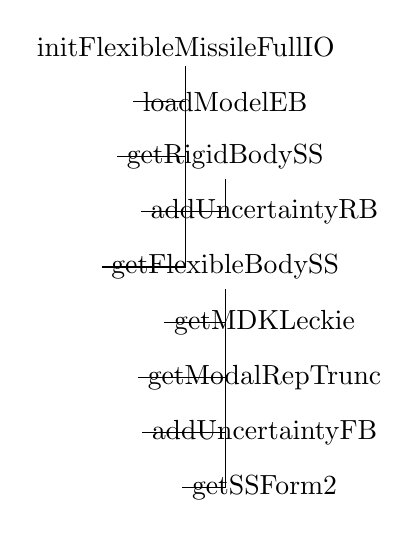
\begin{tikzpicture}[% 
grow via three points={one child at (0.5,-0.7) and  
two children at (0.5,-0.7) and (0.5,-1.4)}, 
edge from parent path={(\tikzparentnode.south) |- (\tikzchildnode.west)}]
\node {initFlexibleMissileFullIO} 
	child { node {loadModelEB}}	    
	child { node {getRigidBodySS}       
		child { node {addUncertaintyRB}}      
	}     
	child [missing] {}	
	child { node {getFlexibleBodySS}       
		child { node {getMDKLeckie}}       
		child { node {getModalRepTrunc}} 
		child { node {addUncertaintyFB}}  
		child { node {getSSForm2}}     
	}     			     
	child [missing] {}				     
	child [missing] {}				     
	child [missing] {}				     
	child [missing] {}; 
\end{tikzpicture}

\par\end{centering}

\caption{Calling Tree - Flexible Missile Modeling\label{fig:Calling-Tree}}
\end{figure}



\subsection{Servo-aeroelastic Model Generation}
\begin{description}
\item [{Filename}] \texttt{initMissileFullIO.m}
\item [{Author}] A. Verhaegen
\item [{Description}] This is the main file to generate the servo-aeroelastic
model.
\item [{Algorithm}] This script will first initialize all structural and
flight parameters with the function \texttt{loadModelEB}. The rigid-body
model, the flexible-body model and the actuators dynamics are derived.
Finally these models are merged in a simulink file at extracted to
the MATLAB workspace.
\item [{Inputs}] None
\item [{Outputs}]~

\begin{lyxlist}{00.00.0000}
\item [{\texttt{missile}}] uncertain state-space system of the missile
\end{lyxlist}
\item [{Calling}] \texttt{loadModelEB}, \texttt{getRigidBodySS}, \texttt{getFlexibleBodySS}
\item [{Called~from}] \texttt{main} 
\end{description}

\subsection{Rigid-body State-space System Generation}
\begin{description}
\item [{Filename}] \texttt{getRigidBodySS.m}
\item [{Author}] A. Verhaegen
\item [{Description}] The function \texttt{getRigidBodySS} generates the
rigid-body state-space system of a missile.
\item [{Algorithm}] The first step is to find the equilibrium. The algorithm
defines symbolic variables to create the three equations of motion.
An approximate solution of the trim is found and feeds the solver
to find a numerical solution for the trim. Once this equilibrium is
found the second step is to compute the state-space matrices A,B,C,D
with uncertainty on $T_{0}$ and $x_{CG}$.
\item [{Inputs}]~

\begin{lyxlist}{00.00.0000}
\item [{\texttt{S}}] reference surface $S_{ref}$
\item [{\texttt{rho}}] air density $\rho$
\item [{\texttt{CL0}}] zero AoA lift coefficient $C_{L0}$
\item [{\texttt{CLa}}] lift coefficient slope $C_{L\alpha}$
\item [{\texttt{CLd}}] fins lift coefficient slope $C_{L\delta_{F}}$
\item [{\texttt{xFins}}] position of the fins from the tail $x_{F}$
\item [{\texttt{xAE}}] position of the aerodynamic centre $x_{AC}$
\item [{\texttt{Cm0}}] zero AoA pitching moment coefficient $C_{m0}$
\item [{\texttt{Cma}}] pitching moment coefficient slope $C_{m\alpha}$
\item [{\texttt{Cmd}}] fins pitching moment coefficient $C_{m\delta_{F}}$
\item [{\texttt{CD0}}] zero lift drag coefficient $C_{D0}$
\item [{\texttt{kD}}] drag coefficient slope $k_{D}$
\item [{\texttt{Dref}}] reference length $L_{ref}$
\item [{\texttt{V0}}] trim speed $V_{0}$
\item [{\texttt{gamm0}}] trim flight path $\gamma_{0}$ 
\item [{\texttt{Vdot0}}] trim acceleration $\dot{V_{0}}$
\item [{\texttt{l}}] beam element length $l$
\item [{\texttt{dm}}] vector of nodes masses $(m_{i})$
\item [{\texttt{listAcc}}] indices of accelerometers (here 10, 53, 83 and
92)
\item [{\texttt{Jy}}] rotational inertia at CG about y-axis $J_{y}$
\item [{\texttt{xCG}}] centre of gravity position $x_{CG}$
\end{lyxlist}
\item [{Outputs}]~

\begin{lyxlist}{00.00.0000}
\item [{\texttt{rigidBody}}] uncertain SS system of the rigid-body
\item [{\texttt{alph0}}] trim AoA $\alpha_{0}$
\item [{\texttt{T0}}] trim thrust $T_{0}$
\item [{\texttt{thetaT0}}] trim thrust orientation $\theta_{T0}$
\end{lyxlist}
\item [{Calling}] \texttt{addUncertaintyRB}
\item [{Called~from}] \texttt{initMissileFullIO}
\end{description}

\subsection{Flexible-body Modeling}
\begin{description}
\item [{Filename}] \texttt{getFlexibleBodySS.m}
\item [{Author}] A. Verhaegen
\item [{Description}] The function \texttt{getFlexibleBodySS} generates
the flexible-body state-space system of a missile.
\item [{Algorithm}] The first step is to find the second order structural
matrices M, D and K using \texttt{getMDKLeckie}. Then the structural
system is formulated under its modal form keeping only a few flexible-body
modes with \texttt{getModalRepTrunc}. Finally after adding uncertainty
on the natural frequencies and the damping ratios, the system is formulated
under its state-space form 2 with \texttt{getSSForm2}.
\item [{Inputs}]~

\begin{lyxlist}{00.00.0000}
\item [{\texttt{EI}}] vector of bending stiffnesses $\left(EI_{i}\right)_{i}$
\item [{\texttt{l}}] beam element length $l$
\item [{\texttt{dm}}] vector of nodes masses $\left(m_{i}\right)_{i}$
\item [{\texttt{Diam}}] vector of diameters at nodes
\item [{\texttt{m}}] total mass $m$
\item [{\texttt{xCG}}] position of CG $x_{CG}$
\item [{\texttt{Jy}}] rotational inertia $J_{y}$
\item [{\texttt{n\_modes}}] number of flexible modes kept (5 here)
\end{lyxlist}
\item [{Outputs}]~

\begin{lyxlist}{00.00.0000}
\item [{\texttt{flexibleBody}}] uncertain SS system of flexible body
\item [{\texttt{Vm}}] transformation matrix of modal form 2 to original
SS
\end{lyxlist}
\item [{Calling}] \texttt{getMDKLeckie}, \texttt{getModalRepTrunc}, \texttt{addUncertaintyFB},
\texttt{getSSForm2}
\item [{Called~from}] \texttt{initMissileFullIO}
\end{description}

\section{Control Design}

The controllers have been implemented in MATLAB with 6 m-files. They
are summarized in Figure \ref{fig:Control} by a calling tree.

\begin{figure}
\begin{centering}
\tikzstyle{every node}=[draw=black,thick,anchor=west,font=\ttfamily]
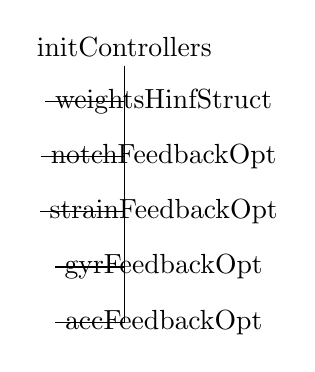
\begin{tikzpicture}[% 
grow via three points={one child at (0.5,-0.7) and  
two children at (0.5,-0.7) and (0.5,-1.4)}, 
edge from parent path={(\tikzparentnode.south) |- (\tikzchildnode.west)}]
\node {initControllers} 
	child { node {weightsHinfStruct}}	 
	child { node {notchFeedbackOpt}}
	child { node {strainFeedbackOpt}}
	child { node {gyrFeedbackOpt}}
	child { node {accFeedbackOpt}}; 
\end{tikzpicture}\caption{Calling Tree - Control Design\label{fig:Control}}

\par\end{centering}

\end{figure}



\subsection{Controllers Initialisation}
\begin{description}
\item [{Filename}] \texttt{initControllers.m}
\item [{Author}] A. Verhaegen
\item [{Description}] The script \texttt{initControllers} creates four
different closed-loop system for the flexible missile using the $H_{\infty}$
structured tuning.
\item [{Algorithm}] After generating the frequency weights with \texttt{weightsHinfStruct},
this script will tune the four different latax controllers (``Notch'',
``Strain'', ``Gyro'', and ``Acc'') with the $H_{\infty}$ structured
tuning in the m-files \texttt{notchFeedbackOpt}, \texttt{strainFeedbackOpt},
\texttt{gyrFeedbackOpt} and \texttt{accFeedbackOpt}.
\item [{Inputs}]~

\begin{lyxlist}{00.00.0000}
\item [{\texttt{missile}}] uncertain state-space system of the missile
\end{lyxlist}
\item [{Outputs}]~

\begin{lyxlist}{00.00.0000}
\item [{\texttt{notchCL}}] closed-loop featured with a notch filter
\item [{\texttt{strainCL}}] closed-loop using the strain measurement
\item [{\texttt{gyrCL}}] closed-loop using the multiple gyroscopes
\item [{\texttt{accCL}}] closed-loop using the multiple accelerometers
\end{lyxlist}
\item [{Calling}] \texttt{weightsHinfStruct}, \texttt{notchFeedbackOpt},
\texttt{strainFeedbackOpt}, \texttt{gyrFeedbackOpt}, \texttt{accFeedbackOpt}
\item [{Called~from}] \texttt{main}
\end{description}

\subsection{H$_{\infty}$ Tuning}
\begin{description}
\item [{Filenames}] \texttt{notchFeedbackOpt.m, strainFeedbackOpt.m, gyrFeedbackOpt.m,
accFeedbackOpt.m}
\item [{Author}] A. Verhaegen
\item [{Description}] These functions create a closed-loop system respectively
for architectures ``Notch'', ``Strain'', ``Gyro'' and ``Acc''.
\item [{Algorithm}] A tunable system is generated using Simulink. This
system is weighted with the frequency weights generated with \texttt{weightsHinfStruct}
and tuned with the H$_{\infty}$ structured tuning method.
\item [{Inputs}]~

\begin{lyxlist}{00.00.0000}
\item [{\texttt{Win}}] input weights
\item [{\texttt{Wout}}] output weights
\item [{\texttt{inputs}}] input names
\item [{\texttt{outputs}}] output names
\end{lyxlist}
\item [{Outputs}]~

\begin{lyxlist}{00.00.0000}
\item [{\texttt{notchCL}}] closed-loop featured with a notch filter
\item [{\texttt{strainCL}}] closed-loop using the strain measurement
\item [{\texttt{gyrCL}}] closed-loop using the multiple gyroscopes
\item [{\texttt{accCL}}] closed-loop using the multiple accelerometers
\end{lyxlist}
\item [{Calling}] None
\item [{Called~from}] \texttt{initControllers}
\end{description}

\chapter{Software Development - Simulink\label{chap:Simulink}}

The servo-aeroelastic model has been designed on Simulink. The models
developed are summarized in a tree on Figure \ref{fig:Simulink-Files-Tree}

\begin{figure}
\centering{}\tikzstyle{every node}=[draw=black,thick,anchor=west,font=\ttfamily]
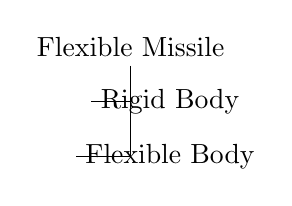
\begin{tikzpicture}[% 
grow via three points={one child at (0.5,-0.7) and  
two children at (0.5,-0.7) and (0.5,-1.4)}, 
edge from parent path={(\tikzparentnode.south) |- (\tikzchildnode.west)}]
\node {Flexible Missile} 
	child { node {Rigid Body}}	
	child { node {Flexible Body}}; 
\end{tikzpicture}\caption{Simulink Files Tree\label{fig:Simulink-Files-Tree}}
\end{figure}



\section{Flexible Missile Model}

Figure \ref{fig:Flexible-Missile-Model-1} is the main model. It creates
the interaction between the flexible body and the rigid body. The
fins and thrust vectoring orientation create two lateral forces that
are the inputs of the flexible body model. These forces create vibrations
in the airframe that are added to the gyroscopes and accelerometer
measurements.

The input $a_{zref}$ (1) is the reference latax to generate. The
inputs $\theta_{Tpert}$ (2) and $\delta_{Fpert}$ (3) are perturbations
on the angles of the actuators. They represent the thrust misalignment
or an error on the fins position. The inputs 4 to 10 are noise sources
on the sensors generated by phenomena that have not been modeled like
white noise or noise created by longitudinal vibrations. The inputs
$\theta_{Tref}$ (11) and $\delta_{Fref}$ (12) are the reference
position of the actuators. They are the control inputs used by the
controller.

Talking about the outputs, $q_{83v}$ (1) and $a_{z83v}$ (2) are
the vibration components of the gyroscope and accelerometer used for
latax control. $\alpha$ (3) is the angle of attack and $a_{zCG}$
(4) is the lateral acceleration of the centre of gravity. $a_{zerr}$
(5) is the error between the reference latax $a_{zref}$ and the CG
latax $a_{zCG}$. $z_{m1}$ (6) is the first bending mode displacement.
The outputs $\theta_{T}$ (7) and $\delta_{F}$ (8) are the angle
of the actuators. These first 8 outputs are not measurements inputs
but they are used to design the controllers and for their assessment.
The outputs 9 to 15 are sensors measurements including the strain
gauge, the gyroscopes and the accelerometers. $\Delta q$ (16) and
$\sum a_{z}$ (17) are signals obtained from linear combinations of
other measurements. The output $a_{zref2}$ (18) is the reference
latax sent to the controller.

\begin{figure}
\begin{centering}
\includegraphics[angle=90,height=0.94\textheight]{figures/simulink/simulinkModel}
\par\end{centering}

\caption{Flexible Missile Model\label{fig:Flexible-Missile-Model-1}}


\end{figure}



\section{Rigid Body Model}

This Simulink model encapsulates the flight dynamics and the actuators
dynamics. It is represented on Figures \ref{fig:Rigid-Body-Model}
and \ref{fig:Flight-Dynamics-Model}.

\begin{figure}
\begin{centering}
\includegraphics[height=0.4\textheight]{figures/simulink/missileSystem}
\par\end{centering}

\caption{Rigid Body Model\label{fig:Rigid-Body-Model}}


\end{figure}


\begin{figure}
\begin{centering}
\includegraphics[height=0.4\textheight]{figures/simulink/missileSystem2}
\par\end{centering}

\caption{Flight Dynamics Model\label{fig:Flight-Dynamics-Model}}
\end{figure}



\section{Flexible Body Model}

The flexible body model is in Figure \ref{fig:Flexible-Body-Model}.
It is based on a discretized Euler Bernoulli beam.

\begin{figure}
\begin{centering}
\includegraphics[height=0.4\textheight]{figures/simulink/flexibleBody}
\par\end{centering}

\caption{Flexible Body Model\label{fig:Flexible-Body-Model}}


\end{figure}


\backmatter

\renewcommand\bibname{References}

\bibliographystyle{ieeetr}
\bibliography{bibliography}

\end{document}
